%%
%% This is file `thesis.tex',
%% generated with the docstrip utility.
%%
%% The original source files were:
%%
%% scnuthesis.dtx  (with options: `thesis')
%% 
%% !Mode:: "TeX:UTF-8"
%% 
%% This is a generated file.
%% 
%% Copyright (C) 2013 by Joseph Pan <cs.wzpan@gmail.com>
%% 
%% This file may be distributed and/or modified under the
%% conditions of the LaTeX Project Public License, either version 1.3a
%% of this license or (at your option) any later version.
%% The latest version of this license is in:
%% 
%% http://www.latex-project.org/lppl.txt
%% 
%% and version 1.3a or later is part of all distributions of LaTeX
%% version 2004/10/01 or later.
%% 
%% To produce the documentation run the original source files ending with `.dtx'
%% through LaTeX.
%% 
%% Any Suggestions : Joseph Pan <cs.wzpan@gmail.com>
%% Thanks LiuBenYuan <liubenyuan@gmail.com> for the nudtpapre class!
%% Thanks Xue Ruini <xueruini@gmail.com> for the thuthesis class!
%% Thanks sofoot for the original NUDT paper class!
%% 
%1. 如果是研究生论文,常用的选项是:
% \documentclass[master,twoside]{scnuthesis}
%2. 如果是博士生论文,常用的选项是:
% \documentclass[doctor,twoside]{scnuthesis}
%3. 如果想生成盲评,传递anon即可,仍需修改个人成果部分
% \documentclass[master,anon]{scnuthesis}
%4. 让章节标题作为页眉,可以使用chapterhead选项。如果和twoside一起使用,则奇数页页眉为章节标题,偶数页为文章标题。
% \documentclass[master,twoside]{scnuthesis}
%
\documentclass[master,twoside]{scnuthesis}
\usepackage{myscnu}

\usepackage{mynewcommand}
\usepackage{listings}
\usepackage{xcolor}
\usepackage{color}
\usepackage{multirow}
\usepackage{booktabs}
\usepackage{enumerate}
\usepackage{amsmath}
\usepackage[colorlinks,linkcolor=black]{hyperref}

\graphicspath {{figures/}}%The folder containing pictures
\captionsetup{font={footnotesize}}
\definecolor{darkgreen}{rgb}{0,0.6,0}
\definecolor{underground}{rgb}{1,1,1}
\definecolor{strcolor}{rgb}{0.8,0,0.8}
\colorlet{stringcolour}{red!60!black}
\colorlet{keywordcolour}{magenta!90!black}
\colorlet{exceptioncolour}{yellow}
\colorlet{commandcolour}{blue!60!black}
\colorlet{numpycolour}{blue!60!green}
\colorlet{literatecolour}{magenta!90!black}
\colorlet{promptcolour}{green!50!black}
\colorlet{specmethodcolour}{violet}
\colorlet{commentcolour}{green!50!black}










\begin{document}
\lstset
{
language=python,
numbers=left,
numberstyle=\color{blue}, 						%代码编号
%stepnumber=0,									%代码编号步长
keywordstyle=\color{keywordcolour}\bfseries,			%关键字颜色
commentstyle=\color{commentcolour},					%注释颜色
%frame=shadowbox,								%边框
breaklines=true, 								%自动折行
stringstyle=\color{stringcolour},				%字符串颜色
backgroundcolor=\color{underground},			%背景色
xleftmargin=0cm,xrightmargin=0cm, aboveskip=1cm, %设置边距
basicstyle=\small,								%基本字体字号  
rulesepcolor=\color{red!20!green!20!blue!20},
flexiblecolumns=true, 
breakautoindent=true,
%python特有关键字
emph={and,break,class,continue,def,yield,del,elif ,else,%
except,exec,finally,for,from,global,if,import,in,%
lambda,not,or,pass,print,raise,return,try,while,assert,with},
emphstyle=\color{blue}\bfseries,
emph={[2]True, False, None},
emphstyle=[2]\color{keywordcolour},
emph={[3]object,type,isinstance,copy,deepcopy,zip,enumerate,reversed,list,len,dict,tuple,xrange,append,execfile,real,imag,reduce,str,repr},
emphstyle=[3]\color{commandcolour},
emph={Exception,NameError,IndexError,SyntaxError,TypeError,FileNotFoundError,ValueError,OverflowError,ZeroDivisionError},
emphstyle=\color{exceptioncolour}\bfseries ,
emph={[4]ode, fsolve, sqrt, exp, sin, cos,arctan, arctan2, arccos, pi,  array, norm, solve, dot, arange, , isscalar, max, sum, flatten, shape, reshape, find, any, all, abs, plot, linspace, legend, quad, polyval,polyfit, hstack, concatenate,vstack,column_stack,empty,zeros,ones,rand,vander,grid,pcolor,eig,eigs,eigvals,svd,qr,tan,det,logspace,roll,min,mean,cumsum,cumprod,diff,vectorize,lstsq,cla,eye,xlabel,ylabel,squeeze},
emphstyle=[4]\color{numpycolour},
emph={[7]range},
emphstyle={[7]\color{keywordcolour}\bfseries},
emph={[8]1, 2, 3, 4, 5, 6, 7, 8, 9, 0},
emphstyle={[8]\color{keywordcolour}\bfseries},
escapeinside=``
}





\graphicspath{{figures/}}
\classification{}  % 分类号
\udc{}             % UDC号
% \mastertype{学术}  % 硕士学位类型(只用于硕士论文)
\confidentiality{公开}  % 密级
\serialno{20142210069}
\title{基于神经网络的花苗分类}
\entitle{Plant Seedling Classification\\ Based on Neural Network}
\displaytitle{基于神经网络的花苗分类}
\author{张泓铨}
\enauthor{Hongquan Zhang}
\subject{信息与计算科学}
\ensubject{Information and Computing Scinece}
\researchfield{理学}
\school{数学科学学院}
\supervisor{杨坦}
\ensupervisor{Tan Yang}
\protitle{讲师}
\zhdate{\zhtoday}

% 插入摘要,制作封面
\ifisanon{}\else{\maketitle}\fi
\frontmatter
%\begin{cabstract}
华南师范大学是一所有着悠久历史和深厚人文底蕴的高等学府,学校地处中国改革开放之%
都——广州,深得岭南开放务实之精神,有着素朴的传统和良好的学风,七十多年来,学校坚%
持师范教育的特色,始终致力于培养人格健全、有思想、有能力、有社会责任感的优秀人才。%

在大学日益参与经济社会发展的新世纪,华南师范大学正以崭新的风貌、开阔的世界眼光,%
不断拓展大学的育人理念,创造良好的教学和包容的学术研究环境,营造丰富的校园文化,%
努力构建特色鲜明、开放式、综合性高水平教学研究型大学。%
\end{cabstract}
\ckeywords{华南师范大学;论文;模板}

\begin{eabstract}
  South China Normal University is an institution of higher education with a
  long history and a rich legacy. Situated in Guangzhou, the open metropolis in
  South China, South China Normal University is imbued with Lingnan's
  pioneering and pragmatic spirits. It has developed a tradition of elegant
  simplicity and fostered a strong learning environment. In the past seventy
  years or so, South China Normal University has preserved its characteristics
  of teacher education and has been devoted to cultivating talents with moral
  integrity, independent thinking, innovative ability and sense of social
  responsibility.

  In the new century in which the institutions of higher education are getting
  increasingly involved in the social and economic development, South China
  Normal University has adopted an international view on education. Having
  broadened its horizon on the key issue of cultivating talents, it has made its
  greatest efforts to create a congenial and harmonious environment for both
  teaching and academic research and has fostered a rich variety of campus
  culture. It aims to build itself into a high-level comprehensive teaching and
  research-oriented university with open distinctive features.
\end{eabstract}
\ekeywords{SCNU; thesis; template}



% 生成目录
\tableofcontents
%\listoftables           % 如果要生成表目录
%\listoffigures          % 如果要生成图目录

\renewcommand{\chapterlabel}{\denotationname} %设置页眉

%\begin{denotation}

\item[SCNU] 华南师范大学 (South China Normal University)
\item[API] 应用程序编程接口  
\item[cluster] 集群
\item[graphic] 图形
\item[communication] 通信
\item[3D] 三维 (Three Dimemsion)
\item[BMP] 位图
\item[PNG] 便携式网络图形 (Portable Network Graphics)
\item[Watershed] 分水岭
\item[GUI] 图形用户界面 (Graphical User Interface)
\item[$E$] 能量
\item[$m$] 质量
\item[$c$] 光速
\item[$P$] 概率
\item[$T$] 时间
\item[$v$] 速度

\end{denotation}
 % 如果要生成符号列表

% 书写正文,可以根据需要增添章节。
\mainmatter
%\chapter{绪论}

\section{本模板的意义}

\subsection{现有的学位论文模板的不足}
学位论文作为高校教学计划中的重要环节,对提高教学质量、培养学生综合应用能力具有十%
分重要的意义。根据国家制定的《科学技术报告、学位论文和学术论文的编写格式》,华南%
师范大学采用Microsoft Word等文字处理系统制作了相应的学位论文模板。然而,在应用这%
些模板的过程中,却出现了几下几种问题\cite{Maddage2009}:
\begin{enumerate}
\item 无法自动处理图表、公式的序号、参考文献引用标号的变动,经常出现因疏忽而前后%
  文体格式不一致的现象;
\item 无法实现论文的格式和内容的有效分离,导致模板的格式很容易被学生无意中修改,%
  从而影响了学位论文规范化管理的质量;
\item 受制于Word版本的兼容性问题,在不同版本的文档之间常会有显示上的出入。%
\end{enumerate}

\subsection{\LaTeX{}的特性}
\TeX{}作为一个功能强大的特别适合于排版科技文献和书籍的格式化排版程序~,其具有以下几点特性:
\begin{enumerate}
\item 强大的宏定义功能。\TeX{}是一种宏命令编程语言,能够处理非常复杂的排版任务,并生成高质量的输出;
\item 方便的自动编号功能。文章、书籍的章、节、段落以及公式、图表、参考文献、页码等均可自动编号;
\item 良好的通用性。\LaTeX{}几乎在所有的计算机操作系统平台上得到实现。\LaTeX{}的源文%
  件可在不同的平台之间自由的交换,而得到的输出是完全相同的。
\end{enumerate}




\subsection{采用\LaTeX{}学位论文模板的意义}
采用\LaTeX{}学位论文模板将有以下几点意义:
\begin{enumerate}
\item 有效地解决以往的\verb|Word|模板中所存在的问题,有助于提高毕业生的学位论文的排版质量;
\item 有助于推动LaTeX在学生群体中的普及,学会使用\LaTeX{}来生成高质量的文档;
\item 课题最终的成果将完全开源,并在Google Code\footnote{项目主页:\url{http://code.google.com/p/scnuthesis/}}上公布。让更多爱好者研究学习,并不断完善,以适应日后的需求。
\end{enumerate}


\section{(1.2 题目)}
绪论内容

绪论内容

绪论内容

绪论内容

绪论内容

绪论内容

\section{(1.3 题目)}
绪论内容

绪论内容

绪论内容

绪论内容

绪论内容

绪论内容

\subsection{(1.3.1 题目)}
绪论内容

绪论内容

绪论内容

绪论内容

\subsection{(1.3.2 题目)}

绪论内容

绪论内容



%\chapter{论文正文}
\label{chap:main}
本章将进入论文排版的正文
主要包括:字体段落,图片表格,公式定理,参考文献四部分。
版面将包括在\scnuthesis{}中使用到的所有格式,模板中自定义命令到或者特有的东西都将被一一介绍,
希望大家能看到对自己有用的东西,方便上手。

为了节省时间,这份说明的内容同样参考了国防科技大学的\nudtpaper{}模板~,在此表示感谢。

\section{字体段落}
\label{sec:font}

本节内容来自华南师范大学外部门户\footnote{外部门户主页:\url{http://www.scnu.edu.cn/}}。

华南师范大学始建于1933年,是一所学科门类齐全的国家“211 工程”重点建设大学和广东%
省省属重点大学。学校现有广州石牌、广州大学城和南海3个校区,占地面积共3079亩,%
校舍面积共 126万平方米。校园环境优美,景色怡人~,人文景观遍布,文化气息浓厚,为广%
大师生提供了良好的学习、工作和生活环境。

学校现有4个国家重点学科(含1个重点培育学科), 9个国家“211 工程”重点建设学%
科,2个广东省一级学科重点学科,11个广东省二级学科重点学科。有71个本科专业,有14个%
博士学位授权一级学科、90个博士学位授权点(未含2011年8月一级学科调整后新增的博士%
点)、1个博士专业学位授权点,33个硕士学位授权一级学科、174个硕士学位授权点(未%
含2011年8月一级学科调整后新增的硕士点)、10个硕士专业学位授权点,涉及到哲学、经济%
学、法学、教育学、文学、历史学、理学、工学、管理学、农学、医学等11个学科门%
类。 有12个博士后流动站。

学校拥有一批实力较强的实验室和科研基地。有教育部激光生命科学重点实验室、环境理论
化学重点实验室(省部共建)、教育部电化学储能材料与技术工程研究中心、卫生部(中医
药管理局)中医药与光子技术实验室、国家理科基础科学研究和教学人才培养基地、教育部
部省共建人文社科重点研究基地(心理应用研究中心)、国家体育总局重点研究基地(体育
社会科学研究基地),有7个广东省重点实验室(中心),6个广东省高校科研型重点实验
室,3个广东省高校产学研结合示范基地,6个广东省普通高校人文社会科学重点研究基
地,1个广东省高校工程技术研究中心。学校还拥有“物理学科基础课”、“信息传
播”~、“心理学”等3个国家级实验教学示范中心,7个广东省实验教学示范中心。此外,教
育部高校辅导员培训和研修基地、广东省普通高等学校师资培训中心~、广东省网络图书馆、
广东高校建筑规划设计院等机构均设在学校。

70 多年来,学校数易校名,几度迁徙,虽历经沧桑,却弦歌不辍。一代又一代华师人秉承勷
勤大学师范学院{\kai “研究高深学术,养成社会之专门人才”}的优良传统,承传南方大
学{\kai “忠诚团结,朴实虚心,勤劳勇敢,实事求是”}的革命精神~,践行{\kai “艰苦奋斗、严谨治
学、求实创新、为人师表”}的校训,筚路蓝缕,薪火相传,共同铸就了学校今天的繁荣与
发展。

华南师范大学历史上的名字包括:

\begin{itemize}
\item[楷体] {\kai 广州市立师范学校}
\item[黑体] {\hei 勷勤大学师范学院}
\item[隶书] {\li 勷勤大学教育学院}
\item[宋体] {\song 广东省立教育学院}
\item[仿宋] {\fs 广东省立文理学院}
\item[粗体] {\bfseries 广东省文理学院}
\item[斜体] {\itshape 华南师范学院}
\item[粗斜体] {\bfseries\itshape 广东师范学院}
\item[字体颜色] {\textcolor{red}{华南师范大学}}
\end{itemize}

上面这段内容使用了itemize列表环境,\LaTeX{}默认的列表环境会在条目之间插入
过多的行距,若用户需要紧凑的行距,可以使用compactitem环境。

下面测试英文字体:

Remember the \textsf{more} \textbf{font} {\bfseries\tiny you \sffamily use,
\Large the \scshape more \itshape beautiful \slshape your \footnotesize
document becomes.}

\begin{itemize}
\item[英文黑体] Typeset text in \textbf{bold} series
\item[英文斜体] Typeset text in \textit{italic} shape
\item[Roman字体] Typeset text in roman family
\item[Sans Serif字体] Typeset text in \textsf{sans serif} family
\item[typewriter字体] Typeset text in \texttt{typewriter} family
\end{itemize}

下面测试字号:
\begin{itemize}
\item[初号] {\chuhao 华南师范大学}
\item[小初] {\xiaochu 华南师范大学}
\item[一号] {\yihao 华南师范大学}
\item[小一] {\xiaoyi 华南师范大学}
\item[二号] {\erhao 华南师范大学}
\item[小二] {\xiaoer 华南师范大学}
\item[三号] {\sanhao 华南师范大学}
\item[小三] {\xiaosan 华南师范大学}
\item[四号] {\sihao 华南师范大学}
\item[小四] {\xiaosi 华南师范大学}
\item[五号] {\wuhao 华南师范大学}
\item[小五] {\xiaowu 华南师范大学}
\end{itemize}

\section{表格明细}
\label{sec:figure}
表格是书中的重要组成部分,这一章将从简单的表格讲起,到复杂的表格为止。

\subsection{基本表格}
\label{sec:basictable}

模板中关于表格的宏包有三个: \textsf{booktabs}、\textsf{array} 和
\textsf{longtabular},命令有一个 \verb|\hlinewd|。三线表建议使用\textsf{booktabs}中提供的,
包含toprule、midrule 和 bottomrule三条命令。
它们与\textsf{longtable} 能很好的配合使用。如果表格比较简单的话可以直接用命令
\verb|hlinewd{xpt}| 控制。下面来看一个表格:
\begin{table}[htb]
  \centering
  \begin{minipage}[t]{0.8\linewidth} % 如果想在表格中使用脚注,minipage是个不错的办法
  \caption[模板文件]{模板文件。如果表格的标题很长,那么在表格索引中就会很不美
    观,所以要像 chapter 那样在前面用中括号写一个简短的标题。这个标题会出现在索
    引中。}
  \label{tab:template-files}
    \begin{tabular*}{\linewidth}{lp{10cm}}
      \toprule[1.5pt]
      {\hei 文件名} & {\hei 描述} \\
      \midrule[1pt]
      scnuthesis.ins & \LaTeX{} 安装文件,docstrip\footnote{表格中的脚注} \\
      scnuthesis.dtx & 所有的一切都在这里面\footnote{再来一个}。\\
      scnuthesis.cls & 模板类文件。\\
      scnuthesis.cfg & 模板配置文。cls 和 cfg 由前两个文件生成。\\
      bstutf8.bst   & 参考文献 Bibtex 样式文件。\\
      myscnu.sty    & 常用的包和命令写在这里,减轻主文件的负担。\\
      \bottomrule[1.5pt]
    \end{tabular*}
  \end{minipage}
\end{table}

如果你不需要在表格中插入脚注,可以将minipage环境去掉。

表 \ref{tab:template-files} 列举了本模板主要文件及其功能。
请大家注意三线表中各条线对应的命令。这个例子还展示了如何在表格中正确使用脚注。
由于 \LaTeX{} 本身不支持在表格中使用 \verb|\footnote|,所以我们不得不将表格放在
小页中,而且最好将表格的宽度设置为小页的宽度,这样脚注看起来才更美观。

如果遇到表格内容自动调整的问题,可以有两种解决办法: 其一就是用\verb|tabular*|,在
两列之间全部插入空白,该方法存在的缺点是当只有两列需要自动调整时,若小页预留空间
过大,可能插入过多的\verb|fill|,导致不美观; 另外一种就是使用\verb|tabularx|自动
调整了,需要定制一个\textbf{Z}环境,在新版本中,该命令已添加到\verb|myscnu.sty|中。
下面是这两个方法实现的对比,各位可以仔细对比一下,推荐使用后者。

\begin{table}[htbp]
\centering
\begin{minipage}[t]{0.9\linewidth}
\caption{Reed Solomon码的典型应用}
\label{tab:RSused}
\begin{tabular*}{\linewidth}{c @{\extracolsep{\fill}} c}
\toprule[1.5pt]
{\hei 应用领域} & {\hei 编码方案}\\
\midrule[1pt]
磁盘驱动器 & RS(32,28,5)码 \footnote{码长为32、维数为28、最小距离为5} \\
CD & 交叉交织RS码(CIRC) \\
DVD & RS(208,192,17)码、RS(182,172,11)码 \\
光纤通信 & RS(255,229,17)码 \\
\bottomrule[1.5pt]
\end{tabular*}
\end{minipage}
\end{table}

\begin{table}[htbp]
\centering
\begin{minipage}[t]{0.9\linewidth}
\caption{Reed Solomon码的典型应用}
\label{tab:RSuse}
\begin{tabularx}{\linewidth}{cZ}
\toprule[1.5pt]
{\hei 应用领域} & {\hei 编码方案}\\
\midrule[1pt]
磁盘驱动器 & RS(32,28,5)码 \footnote{码长为32、维数为28、最小距离为5} \\
CD & 交叉交织RS码(CIRC) \\
DVD & RS(208,192,17)码、RS(182,172,11)码 \\
光纤通信 & RS(255,229,17)码 \\
\bottomrule[1.5pt]
\end{tabularx}
\end{minipage}
\end{table}

\subsection{复杂表格}
\label{sec:complicatedtable}

我们经常会在表格下方标注数据来源,或者对表格里面的条目进行解释。前面的脚注是一种
不错的方法,如果你不喜欢脚注。那么完全可以在表格后面自己写注释,比如表~\ref{tab:tabexamp1}。
\begin{table}[htbp]
  \centering
  \caption{复杂表格示例 1}
  \label{tab:tabexamp1}
  \begin{minipage}[t]{0.8\textwidth} 
    \begin{tabularx}{\linewidth}{|l|X|X|X|X|}
      \hline
      \multirow{2}*{\backslashbox{x}{y}}  & \multicolumn{2}{c|}{First Half} & \multicolumn{2}{c|}{Second Half}\\
      \cline{2-5}
      & 1st Qtr &2nd Qtr&3rd Qtr&4th Qtr \\ 
      \hline
      East$^{*}$ &   20.4&   27.4&   90&     20.4 \\
      West$^{**}$ &   30.6 &   38.6 &   34.6 &  31.6 \\ 
      \hline
    \end{tabularx}\\[2pt]
    \footnotesize
    *:东部\\
    **:西部
  \end{minipage}
\end{table}

此外,表~\ref{tab:tabexamp1} 同时还演示了另外两个功能:1)通过 \textsf{tabularx} 的
 \texttt{|X|} 扩展实现表格自动放大;2)通过命令 \verb|\backslashbox| 在表头部分
插入反斜线。

为了使我们的例子更接近实际情况,我会在必要的时候插入一些“无关”文字,以免太多图
表同时出现,导致排版效果不太理想。

学校七十余载薪火相传,名师荟萃,著名的教育家罗浚、汪德亮,五四新诗开创者之一康白
情,古代文学家李镜池,古汉语学家吴三立,历史学家王越,逻辑学家李匡武,心理学家阮
镜清,教育学家叶佩华、朱勃,数学家叶述武,物理学家黄友谋、刘颂豪,著名体育教育家
袁浚等众多名家、名师先后在此执教。该校虽数度易名、几经迁徙,但一代又一代华师人秉
承勷勤大学师范学院``研究高深学术,养成社会之专门人才''的优良传统,承传南方大
学``忠诚团结,实事求是''的革命精神,践行``艰苦奋斗、严谨治学、求实创新、为人师
表''的校训,不断推动学校事业向前发展。特别是改革开放以来,抓住科教兴国、人才强国
的发展机遇,凭借建设文化省、教育强省和国家``211工程''的强劲东风,形成了学校现在
跨越式发展的大好局面。

不可否认 \LaTeX{} 的表格功能没有想象中的那么强大,不过只要你足够认真,足够细致,那么
同样可以排出来非常复杂非常漂亮的表格。请参看表~\ref{tab:tabexamp2}。
\begin{table}[htbp]
  \centering\dawu[1.3]
  \caption{复杂表格示例 2}
  \label{tab:tabexamp2}
  \begin{tabular}[c]{|c|m{0.8in}|c|c|c|c|c|}\hline
    \multicolumn{2}{|c|}{Network Topology} & \# of nodes & 
    \multicolumn{3}{c|}{\# of clients} & Server \\\hline
    GT-ITM & Waxman Transit-Stub & 600 &
    \multirow{2}{2em}{2\%}& 
    \multirow{2}{2em}{10\%}& 
    \multirow{2}{2em}{50\%}& 
    \multirow{2}{1.2in}{Max. Connectivity}\\\cline{1-3}
    \multicolumn{2}{|c|}{Inet-2.1} & 6000 & & & &\\\hline
    \multirow{2}{1in}{Xue} & Rui  & Ni &\multicolumn{4}{c|}{\multirow{2}*{\scnuthesis}}\\\cline{2-3}
    & \multicolumn{2}{c|}{ABCDEF} &\multicolumn{4}{c|}{} \\\hline
\end{tabular}
\end{table}

\subsection{子表格与跨页表格}

浮动体的并排放置一般有两种情况:1)二者没有关系,为两个独立的浮动体;2)二者隶属
于同一个浮动体。对表格来说并排表格既可以像图~\ref{tab:parallel1}、图~\ref{tab:parallel2} 
使用小页环境,也可以如图~\ref{tab:subtable} 使用子表格来做。后面我们将讲解图的例子。
\begin{table}[htb]
\noindent\begin{minipage}{0.45\textwidth}
\centering
\caption{第一个并排子表格}
\label{tab:parallel1}
\begin{tabular}{p{2cm}p{2cm}}
\toprule[1.5pt]
111 & 222 \\\midrule[1pt]
222 & 333 \\\bottomrule[1.5pt]
\end{tabular}
\end{minipage}
\begin{minipage}{0.45\textwidth}
\centering
\caption{第二个并排子表格}
\label{tab:parallel2}
\begin{tabular}{p{2cm}p{2cm}}
\toprule[1.5pt]
111 & 222 \\\midrule[1pt]
222 & 333 \\\bottomrule[1.5pt]
\end{tabular}
\end{minipage}
\end{table}

学校教师队伍结构良好、水平较高,拥有一批在国内外具有一定影响的专家学者。现有教师
队伍 1900 多人,其中教授 400 多人,副教授 500 多人,博士、硕士研究生导师 800 多人,
具有博士、硕士学位和研究生学历的1500 多人。在师资队伍中,有中国科学院院士 7 人、
瑞典皇家科学院院士2人、“千人计划”入围者 1人、长江学者4人、获得国家杰出青年基金
项目资助者3人、“新世纪百千万人才”国家级人选 5人、国家级教学名师2 人、广东省领军
人才4人、珠江学者4人、广东省高等学校“千百十工程”国家级培养对象5人,拥有教育
部“长江学者与创新团队发展计划”创新团队 1个、广东省创新科研团队1个,并有国务院学
位委员会学科评议组成员 3 人、教育部高等学校教学指导委员会成员 12 人。

\begin{table}[htbp]
\centering
\caption{并排子表格}
\label{tab:subtable}
\subfloat[第一个子表格]{
\begin{tabular}{p{2cm}p{2cm}}
\toprule[1.5pt]
111 & 222 \\\midrule[1pt]
222 & 333 \\\bottomrule[1.5pt]
\end{tabular}}\hskip2cm
\subfloat[第二个子表格]{
\begin{tabular}{p{2cm}p{2cm}}
\toprule[1.5pt]
111 & 222 \\\midrule[1pt]
222 & 333 \\\bottomrule[1.5pt]
\end{tabular}}
\end{table}

如果您要排版的表格长度超过一页,那么推荐使用 \textsf{longtable} 或者 \textsf{supertabular} 
宏包,表~\ref{tab:performance} 就是 \textsf{longtable} 的简单示例。
\begin{longtable}[c]{c*{6}{r}}
\caption{实验数据}\label{tab:performance}\\
\toprule[1.5pt]
 测试程序 & \multicolumn{1}{c}{正常运行} & \multicolumn{1}{c}{同步}
& \multicolumn{1}{c}{检查点}   & \multicolumn{1}{c}{卷回恢复}
& \multicolumn{1}{c}{进程迁移} & \multicolumn{1}{c}{检查点} 	\\
& \multicolumn{1}{c}{时间 (s)} & \multicolumn{1}{c}{时间 (s)}
& \multicolumn{1}{c}{时间 (s)} & \multicolumn{1}{c}{时间 (s)}
& \multicolumn{1}{c}{时间 (s)} &  文件(KB)			\\
\midrule[1pt]%
\endfirsthead%

\multicolumn{7}{c}{续表~\thetable\hskip1em 实验数据}\\

\toprule[1.5pt]
 测试程序 & \multicolumn{1}{c}{正常运行} & \multicolumn{1}{c}{同步} 
& \multicolumn{1}{c}{检查点}   & \multicolumn{1}{c}{卷回恢复}
& \multicolumn{1}{c}{进程迁移} & \multicolumn{1}{c}{检查点} 	\\
& \multicolumn{1}{c}{时间 (s)} & \multicolumn{1}{c}{时间 (s)}
& \multicolumn{1}{c}{时间 (s)} & \multicolumn{1}{c}{时间 (s)}
& \multicolumn{1}{c}{时间 (s)} &  文件(KB)			\\
\midrule[1pt]%
\endhead%
\hline%

\multicolumn{7}{r}{续下页}%

\endfoot%
\endlastfoot%
CG.A.2 & 23.05   & 0.002 & 0.116 & 0.035 & 0.589 & 32491  \\
CG.A.4 & 15.06   & 0.003 & 0.067 & 0.021 & 0.351 & 18211  \\
CG.A.8 & 13.38   & 0.004 & 0.072 & 0.023 & 0.210 & 9890   \\
CG.B.2 & 867.45  & 0.002 & 0.864 & 0.232 & 3.256 & 228562 \\
CG.B.4 & 501.61  & 0.003 & 0.438 & 0.136 & 2.075 & 123862 \\
CG.B.8 & 384.65  & 0.004 & 0.457 & 0.108 & 1.235 & 63777  \\
MG.A.2 & 112.27  & 0.002 & 0.846 & 0.237 & 3.930 & 236473 \\
MG.A.4 & 59.84   & 0.003 & 0.442 & 0.128 & 2.070 & 123875 \\
MG.A.8 & 31.38   & 0.003 & 0.476 & 0.114 & 1.041 & 60627  \\
MG.B.2 & 526.28  & 0.002 & 0.821 & 0.238 & 4.176 & 236635 \\
MG.B.4 & 280.11  & 0.003 & 0.432 & 0.130 & 1.706 & 123793 \\
MG.B.8 & 148.29  & 0.003 & 0.442 & 0.116 & 0.893 & 60600  \\
LU.A.2 & 2116.54 & 0.002 & 0.110 & 0.030 & 0.532 & 28754  \\
LU.A.4 & 1102.50 & 0.002 & 0.069 & 0.017 & 0.255 & 14915  \\
LU.A.8 & 574.47  & 0.003 & 0.067 & 0.016 & 0.192 & 8655   \\
LU.B.2 & 9712.87 & 0.002 & 0.357 & 0.104 & 1.734 & 101975 \\
LU.B.4 & 4757.80 & 0.003 & 0.190 & 0.056 & 0.808 & 53522  \\
LU.B.8 & 2444.05 & 0.004 & 0.222 & 0.057 & 0.548 & 30134  \\
EP.A.2 & 123.81  & 0.002 & 0.010 & 0.003 & 0.074 & 1834   \\
EP.A.4 & 61.92   & 0.003 & 0.011 & 0.004 & 0.073 & 1743   \\
EP.A.8 & 31.06   & 0.004 & 0.017 & 0.005 & 0.073 & 1661   \\
EP.B.2 & 495.49  & 0.001 & 0.009 & 0.003 & 0.196 & 2011   \\
EP.B.4 & 247.69  & 0.002 & 0.012 & 0.004 & 0.122 & 1663   \\
EP.B.8 & 126.74  & 0.003 & 0.017 & 0.005 & 0.083 & 1656   \\
\bottomrule[1.5pt]
\end{longtable}

为了排版方便,这里要插入一些随机的文字,那就加上猩猩博客的东西吧: 
``越来越喜欢吃,自己做的川菜,每次做菜,都像是创作的过程,%
随心所欲; 发现家常菜真的很难做好,越是简单的菜,越是难以做好。
献上一个鱼香肉丝,让我跟随简单的脚步,creat出简约的菜品。''

\subsection{其它}
\label{sec:tableother}
有的同学不想让某个表格或者图片出现在索引里面,那么请使用命令 \verb|\caption*{}|,
这个命令不会给表格编号,也就是出来的只有标题文字而没有“表~XX”,“图~XX”,否则
索引里面序号不连续就显得不伦不类,这也是 \LaTeX{} 里星号命令默认的规则。

\section{绘图插图}

绘图工具分为 GUI 的和 CLI 两种。GUI即是所见即所得的绘图工具~,常见的包
括 Visio、Inkscape、CorelDraw、XFig(jFig)、WinFig、Tpx、Ipe、Dia等;CLI则是需要编
译后才能够得到图形的工具,比较流行的有 PGF/TikZ~、Asymptote、pstricks等。GUI 类绘
图工具比较易于上手,而 CLI 类绘图工具则能够画出更加精确的图形。关于各类绘图工具的
比较和使用方法~,推荐用户到C\TeX{}论坛{\url{http://bbs.ctex.org/}}以及China\TeX{}论坛
{\url{http://bbs.chinatex.org/forum.php}}上的相关板块进行更加深入的了解。

\subsection{插图}
\label{sec:graphs}

强烈推荐《\LaTeXe 插图指南》!关于子图形使用细节请参看\textsf{subfig}手册。 

\subsubsection{一个图形}
\label{sec:onefig}
一般图形都是处在浮动环境中。之所以称为浮动是指最终排版效果图形的位置不一定与源文
件中的位置对应,这也是刚使
用 \LaTeX{} 同学可能遇到的问题。如果要强制固定浮动图形的位置,请使用 \textsf{float} 宏包,
它提供了 \texttt{[H]} 参数,但是除非特别需要,不建议使用\texttt{[H]},
而是倾向于使用\texttt{[htbp]},给\LaTeX{}更多选择。比如图~\ref{fig:ipe}。
\begin{figure}[htbp] % use float package if you want it here
  \centering
  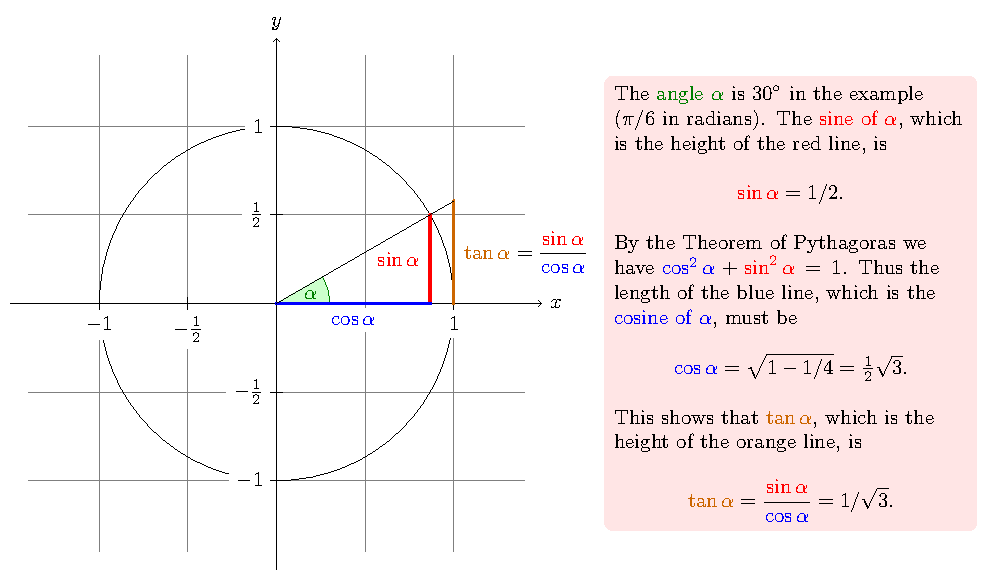
\includegraphics[width=\textwidth]{tikz}
  \caption{利用TikZ制图}
  \label{fig:ipe}
\end{figure}

大学之道,在明明德,在亲民,在止于至善。知止而后有定;定而后能静;静而后能安;安
而后能虑;虑而后能得。物有本末,事有终始。知所先后,则近道矣。古之欲明明德于天
下者,先治其国;欲治其国者,先齐其家;欲齐其家者~,先修其身;欲修其身者,先正其心;
欲正其心者,先诚其意;欲诚其意者~,先致其知;致知在格物。物格而后知至;知至而后
意诚;意诚而后心正;心正而后身修;身修而后家齐;家齐而后国治;国治而后天下
平。自天子以至于庶人,壹是皆以修身为本。其本乱而未治者 否矣。其所厚者薄,而其所
薄者厚,未之有也!

\hfill \pozhehao《大学》

\subsubsection{多个图形}
\label{sec:multifig}

如果多个图形相互独立,并不共用一个图形计数器,那么用 \verb|minipage| 或者
\verb|parbox| 就可以。否则,请参看图~\ref{fig:big1},它包含两个小图,分别是图~\ref{fig:subfig1} 
和图~\ref{fig:subfig2}。推荐使用 \verb|\subfloat|,不要再用
\verb|\subfigure| 和 \verb|\subtable|。
\begin{figure}[htb]
  \centering%
  \subfloat[第一个小图形]{%
    \label{fig:subfig1}
    
\includegraphics[height=2cm]{logo.jpg}}\hspace{4em}%
  \subfloat[第二个小图形。如果标题很长的话,它会自动换行,这个 caption 就是这样的例子]{%
    \label{fig:subfig2}
    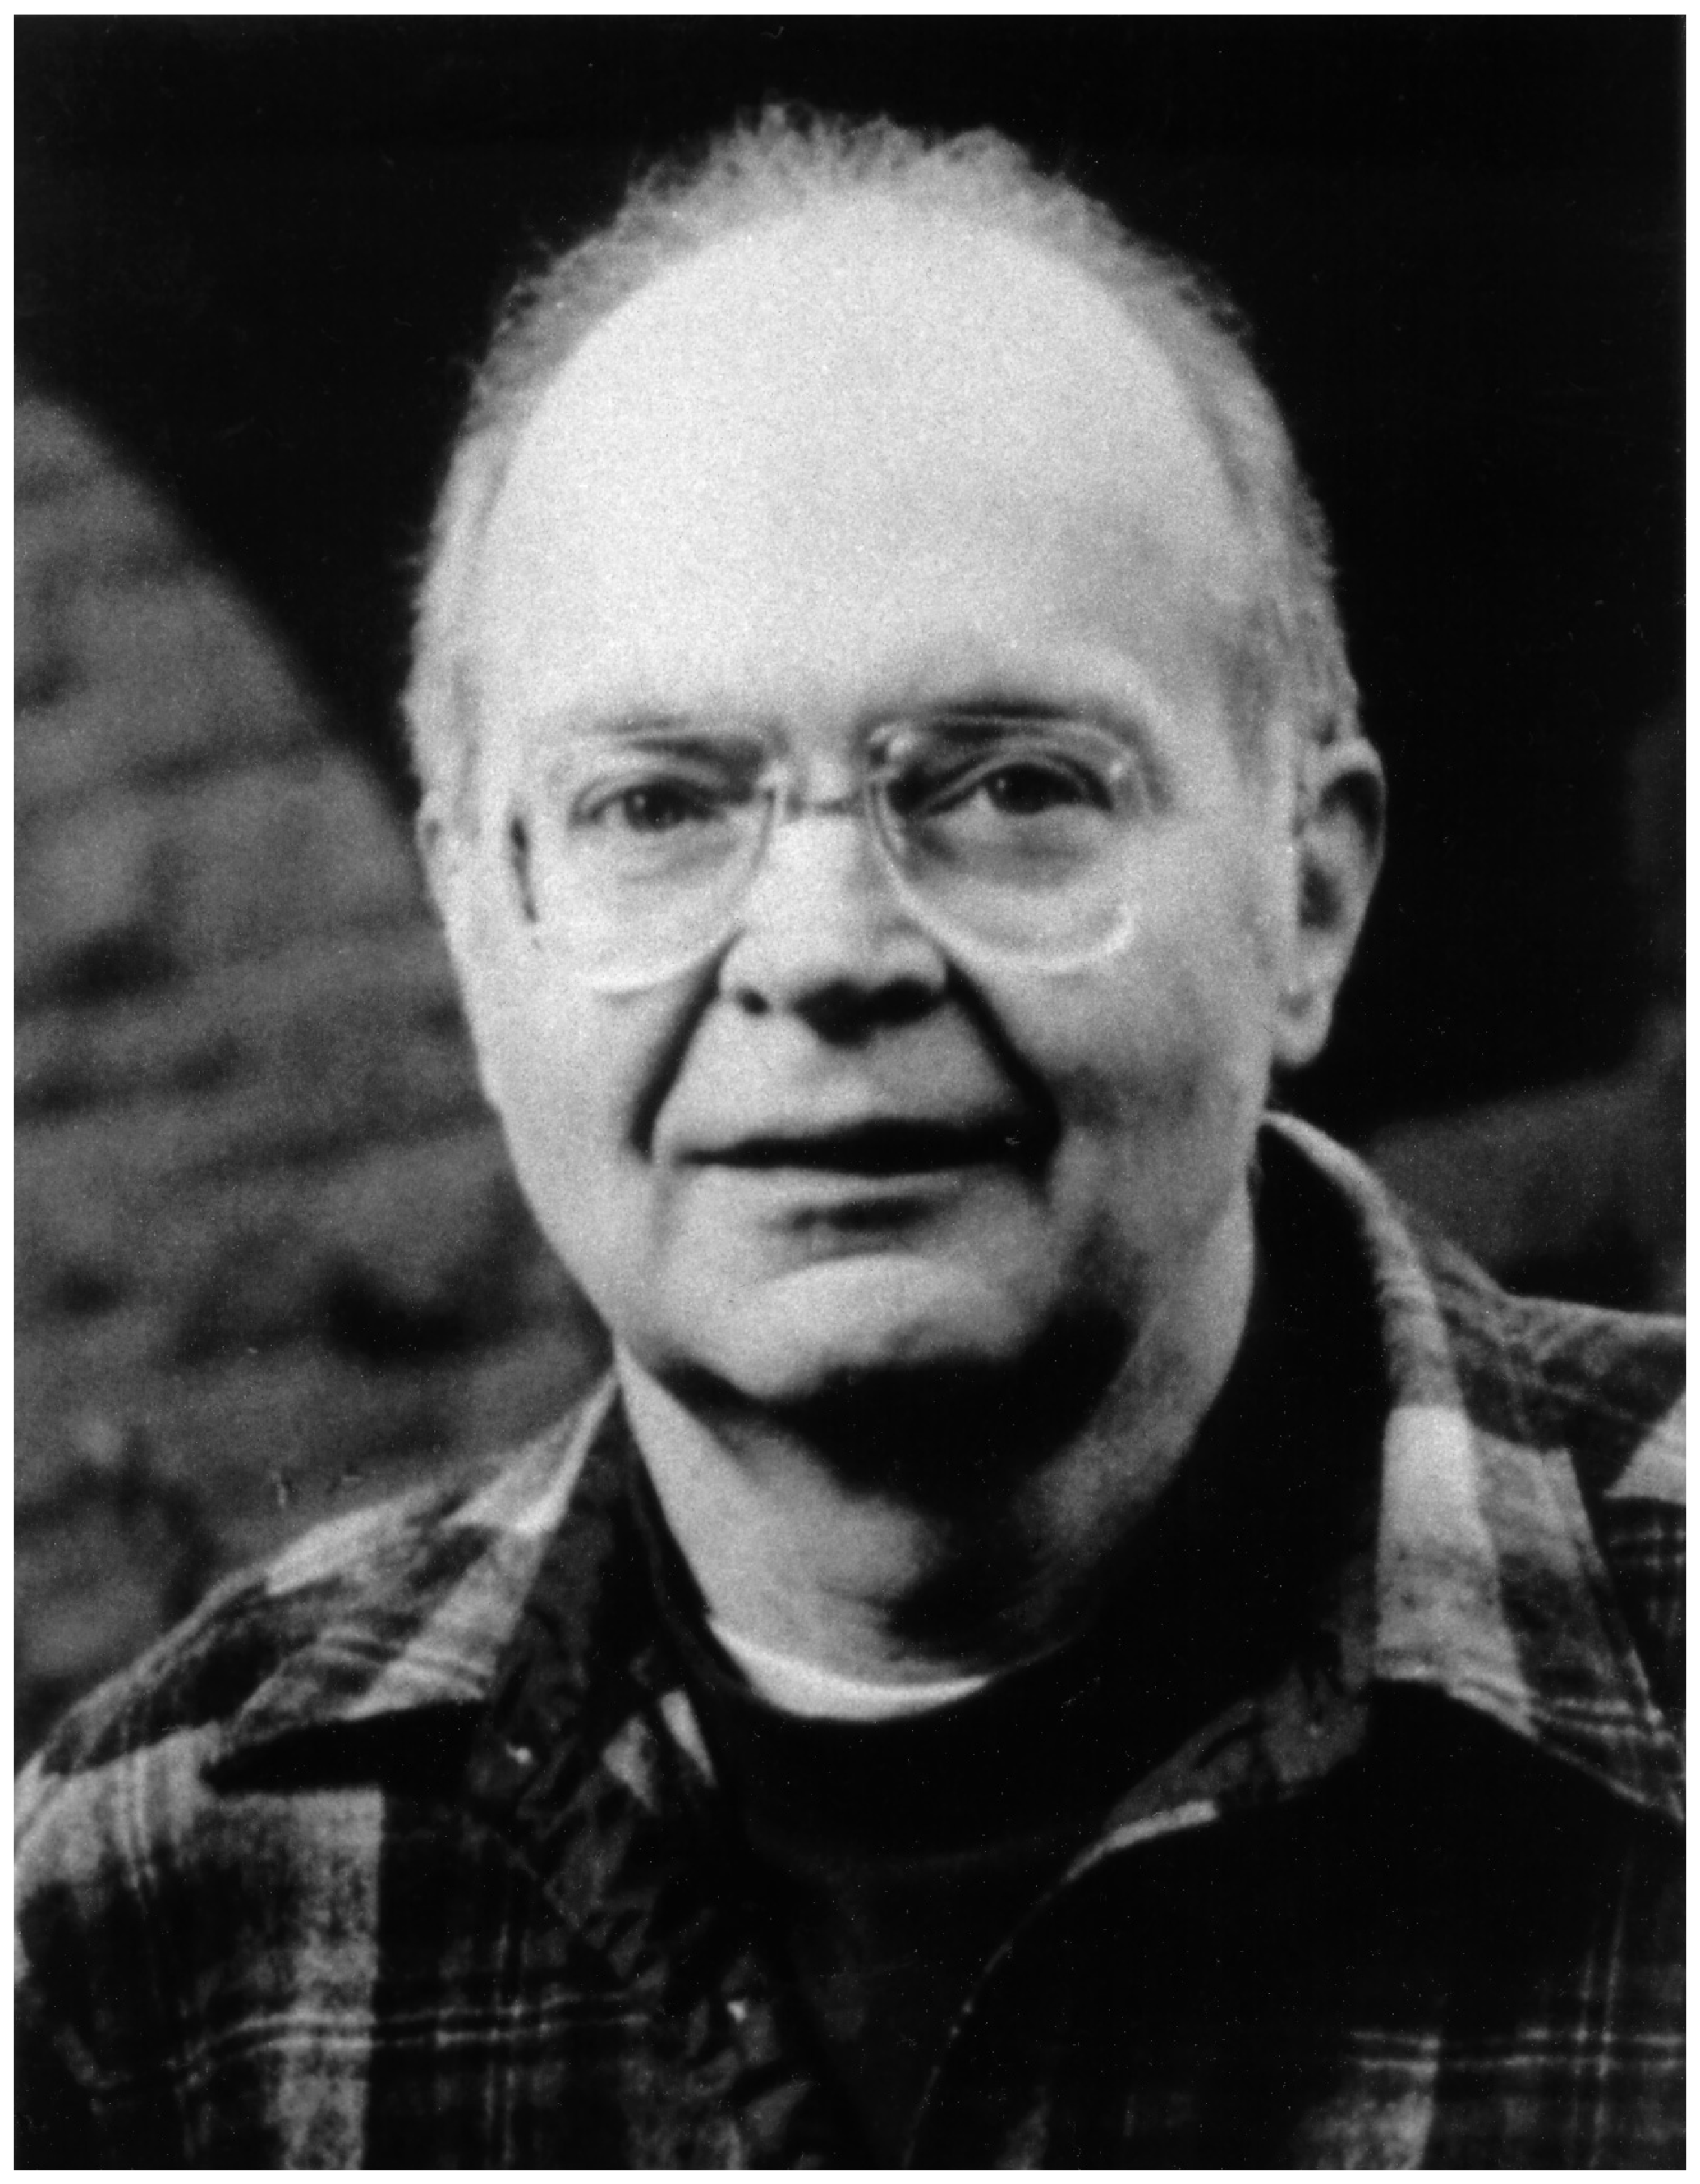
\includegraphics[height=2cm]{don-hires}}
  \caption{包含子图形的大图形}
  \label{fig:big1}
\end{figure}

培育英才万万千,建设祖国锦绣河山,华师儿女奋勇当先,珠江滚滚红绵艳~,岭南大地草木
春,改革开放阳光好,华师园里花烂漫。

艰苦奋斗众志坚,严谨治学成风范,求实创新勇开拓,为人师表代代相传,教育改革宏图展,
师范园地好摇篮,培育祖国栋梁材,神圣职责我承担。


下面这个例子显示并排$3\times2$的图片,见图\ref{fig:subfig:3x2}:
\begin{figure}[htb]
\centering
\subfloat[]{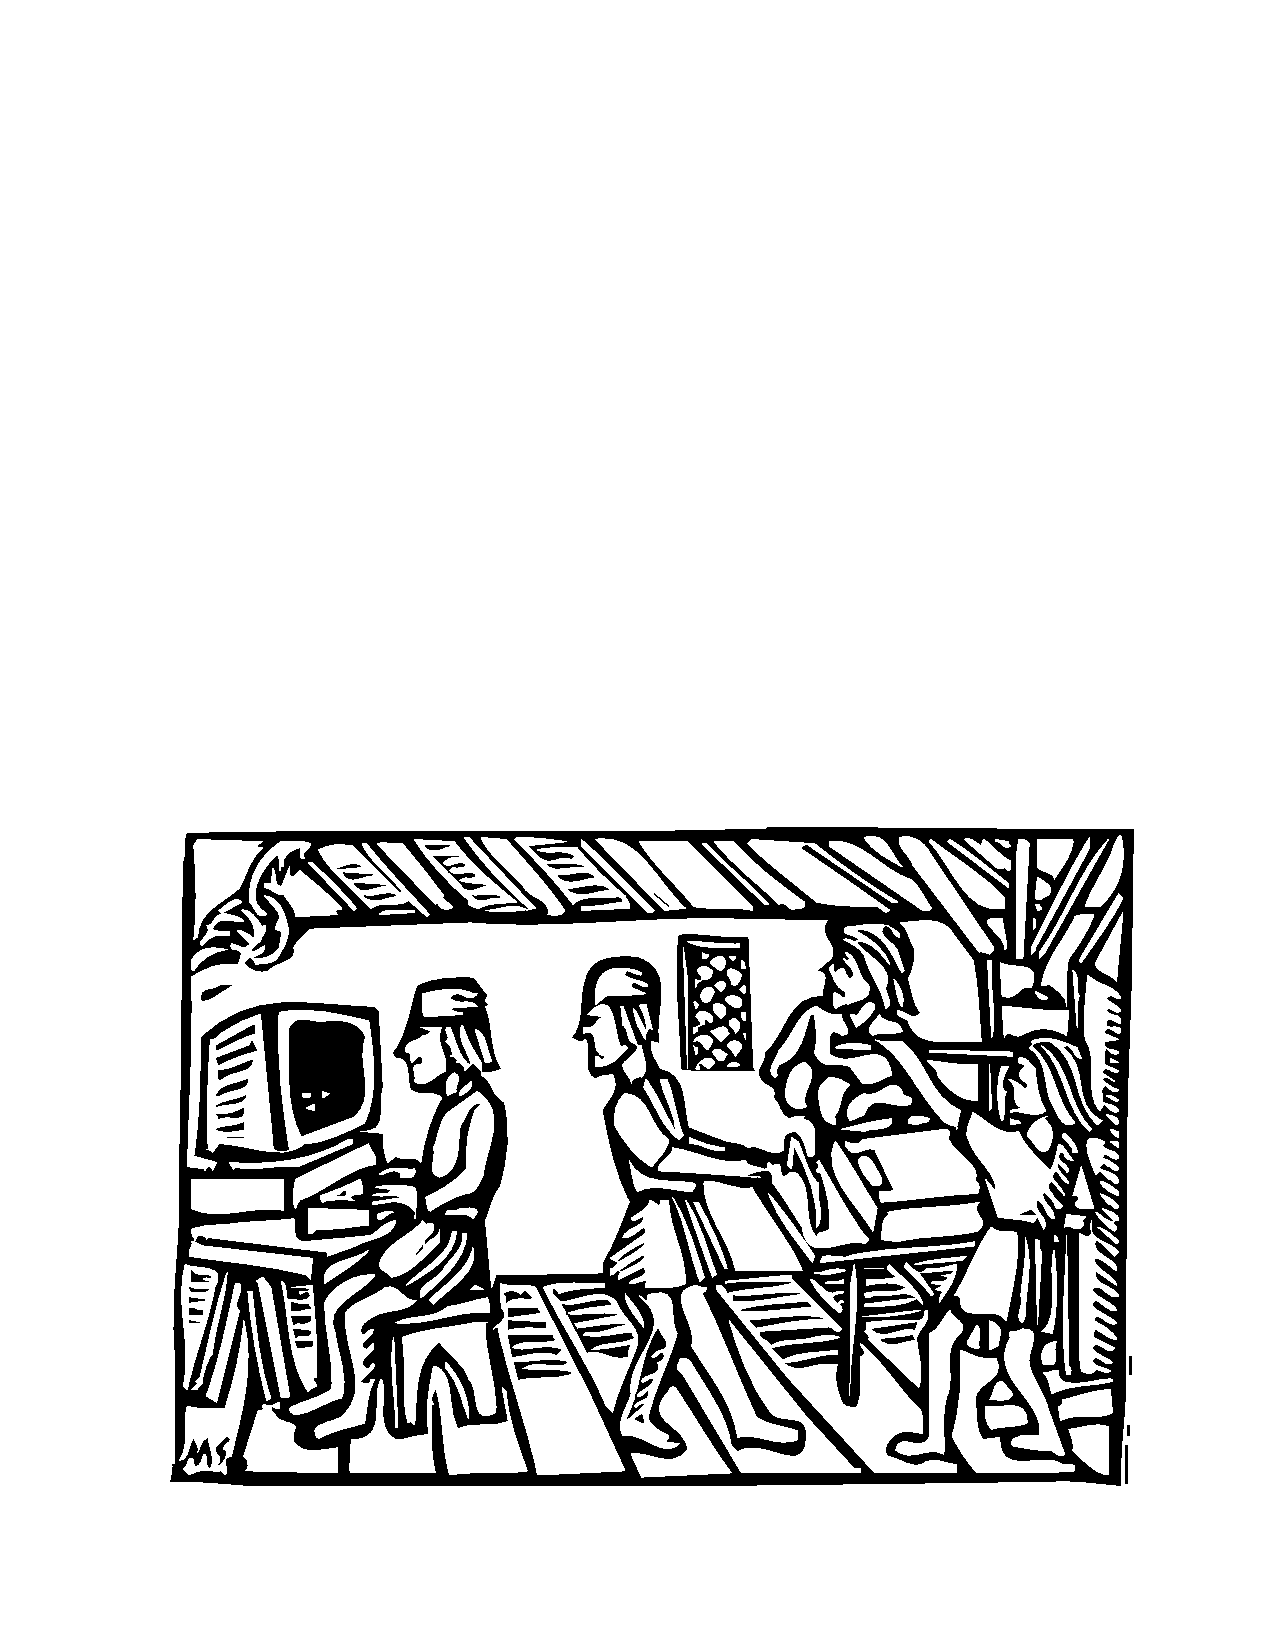
\includegraphics[width=.27\textwidth]{typography}} \qquad
\subfloat[]{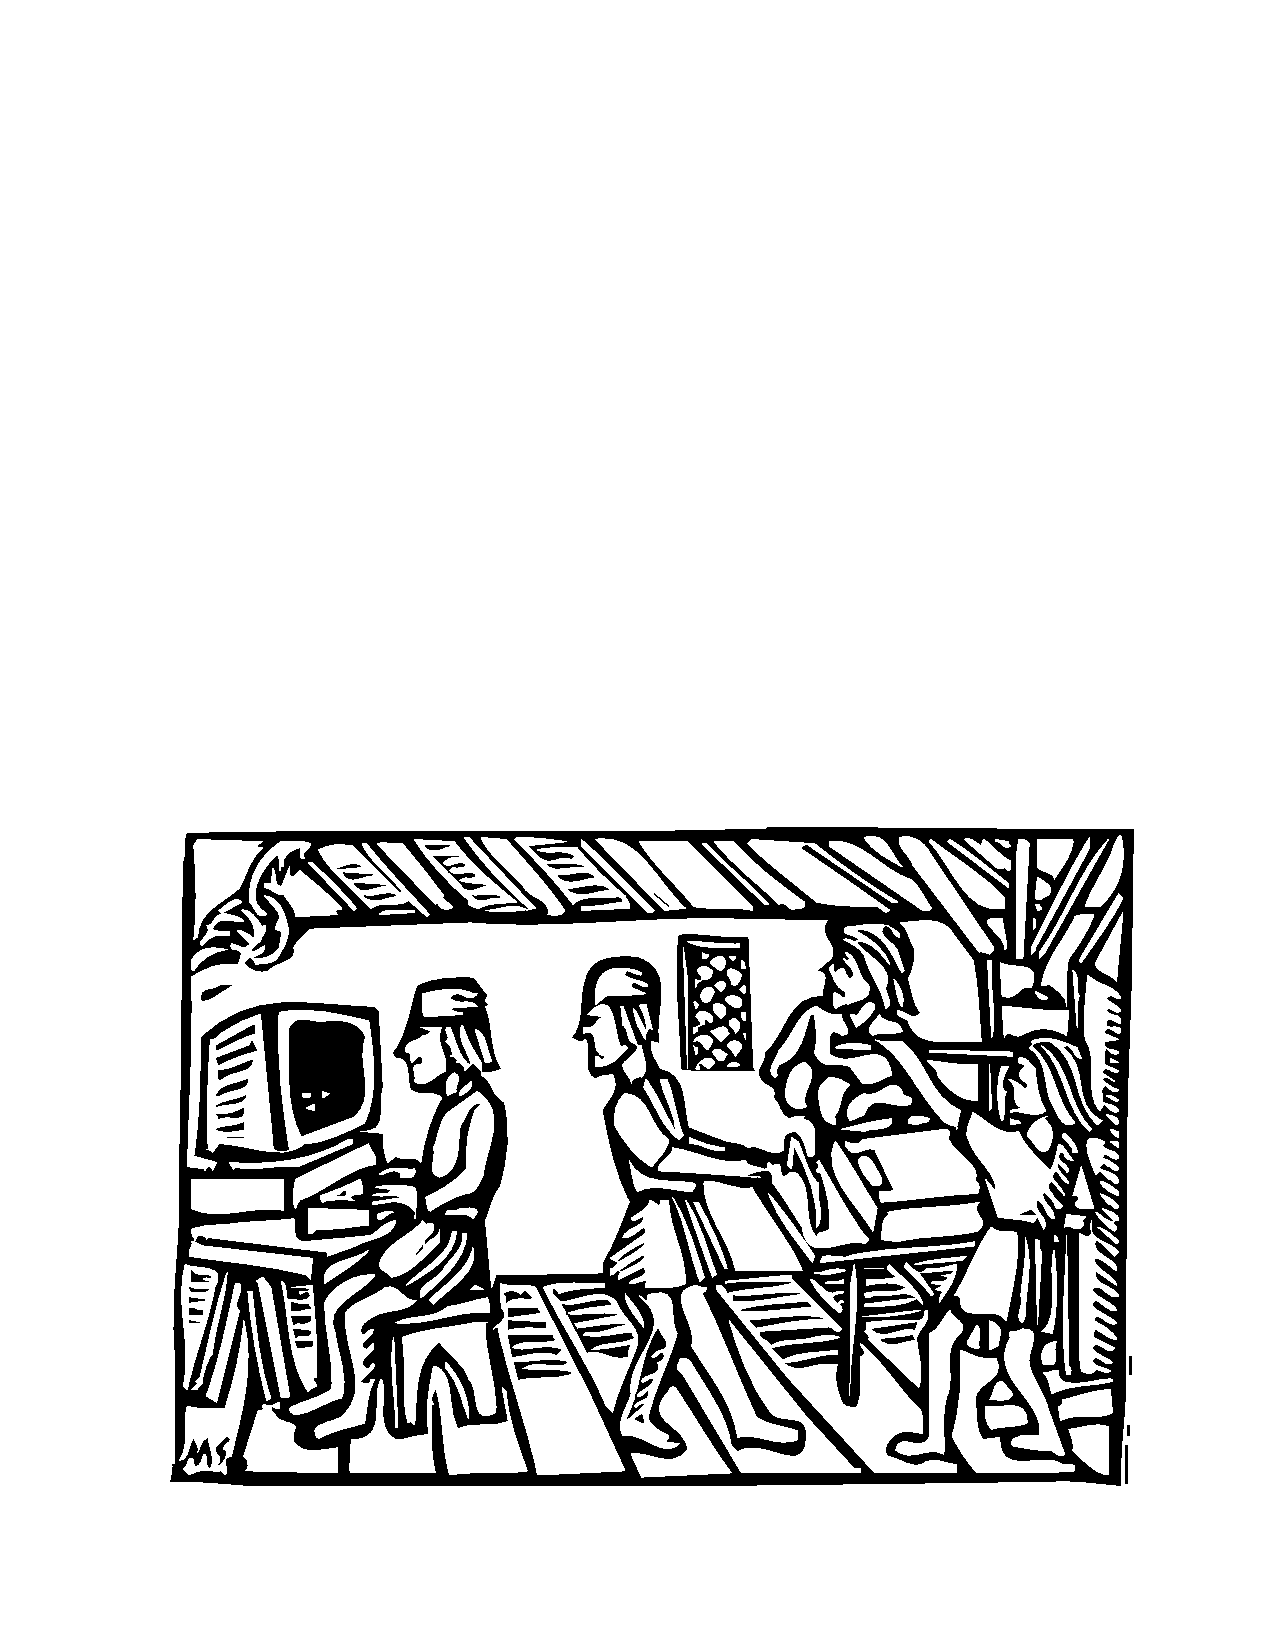
\includegraphics[width=.27\textwidth]{typography}} \qquad
\subfloat[]{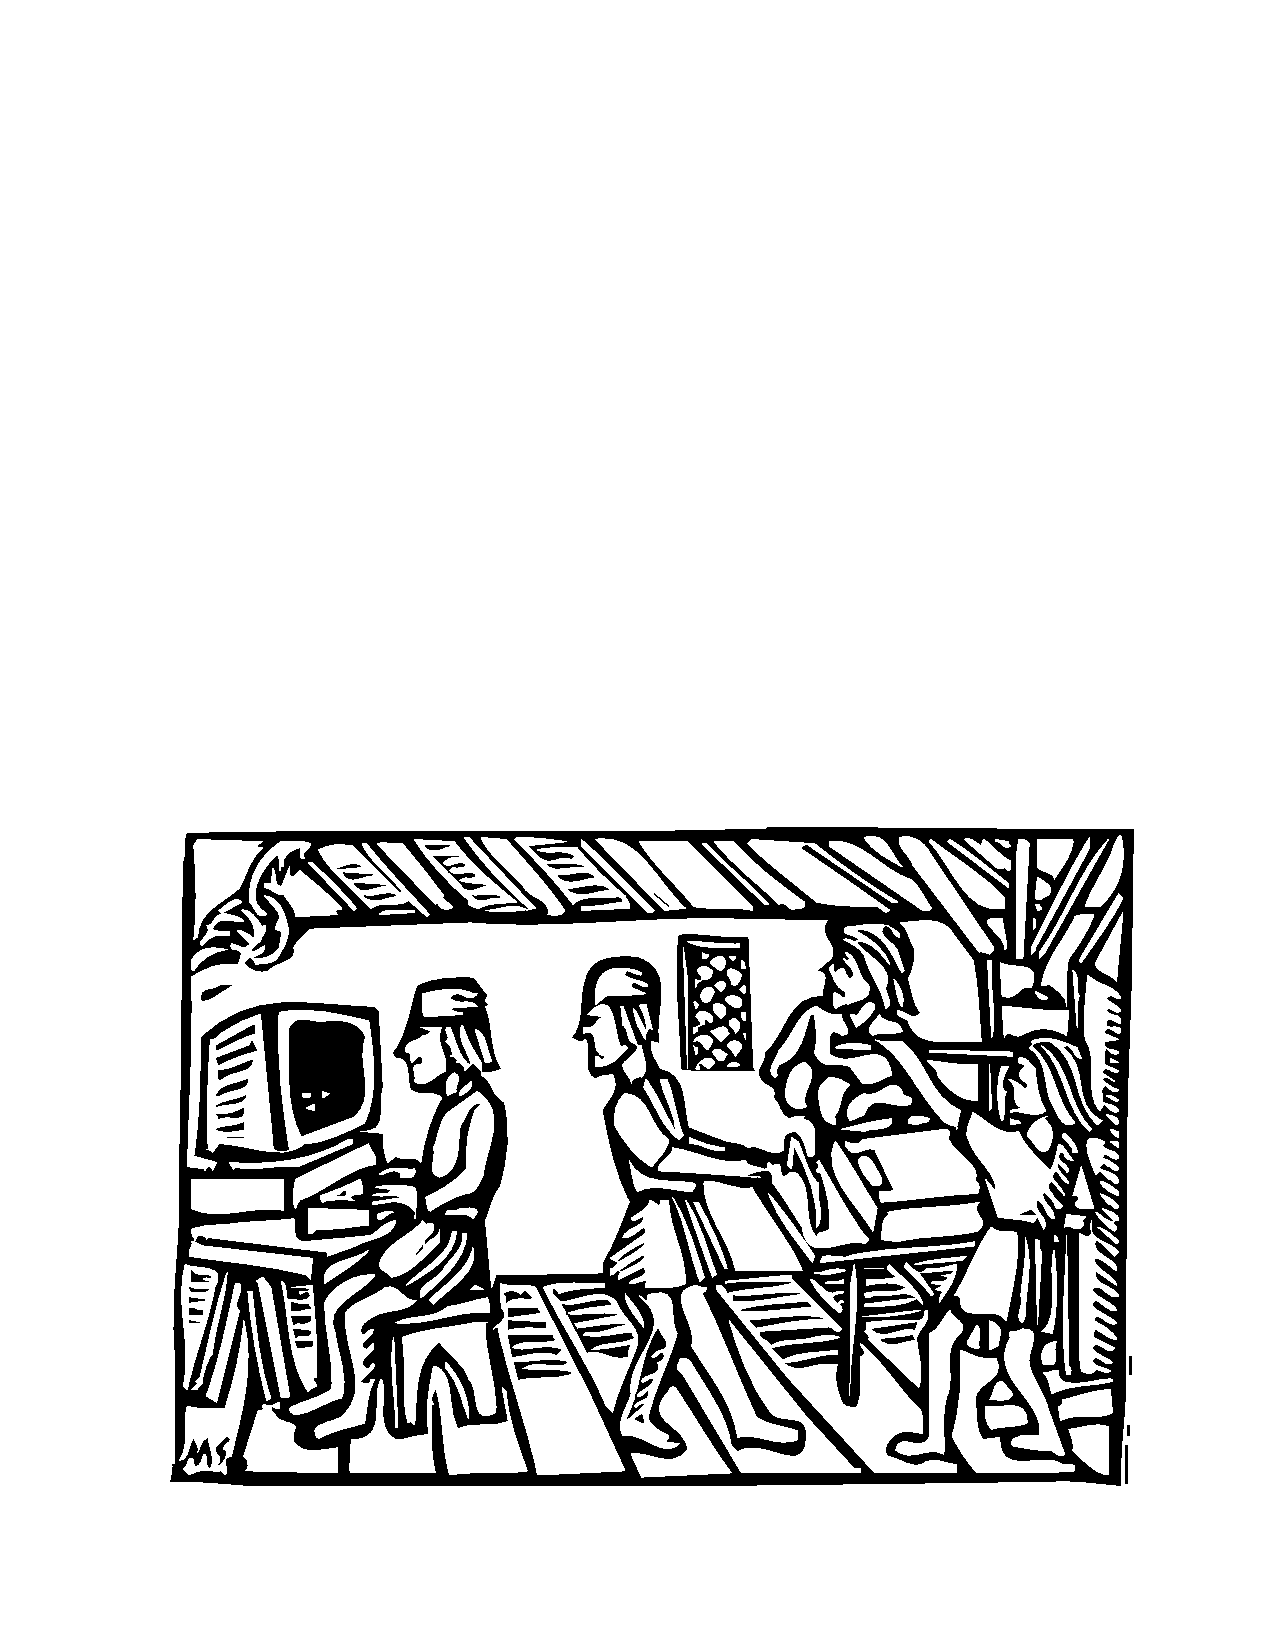
\includegraphics[width=.27\textwidth]{typography}} \qquad
\subfloat[]{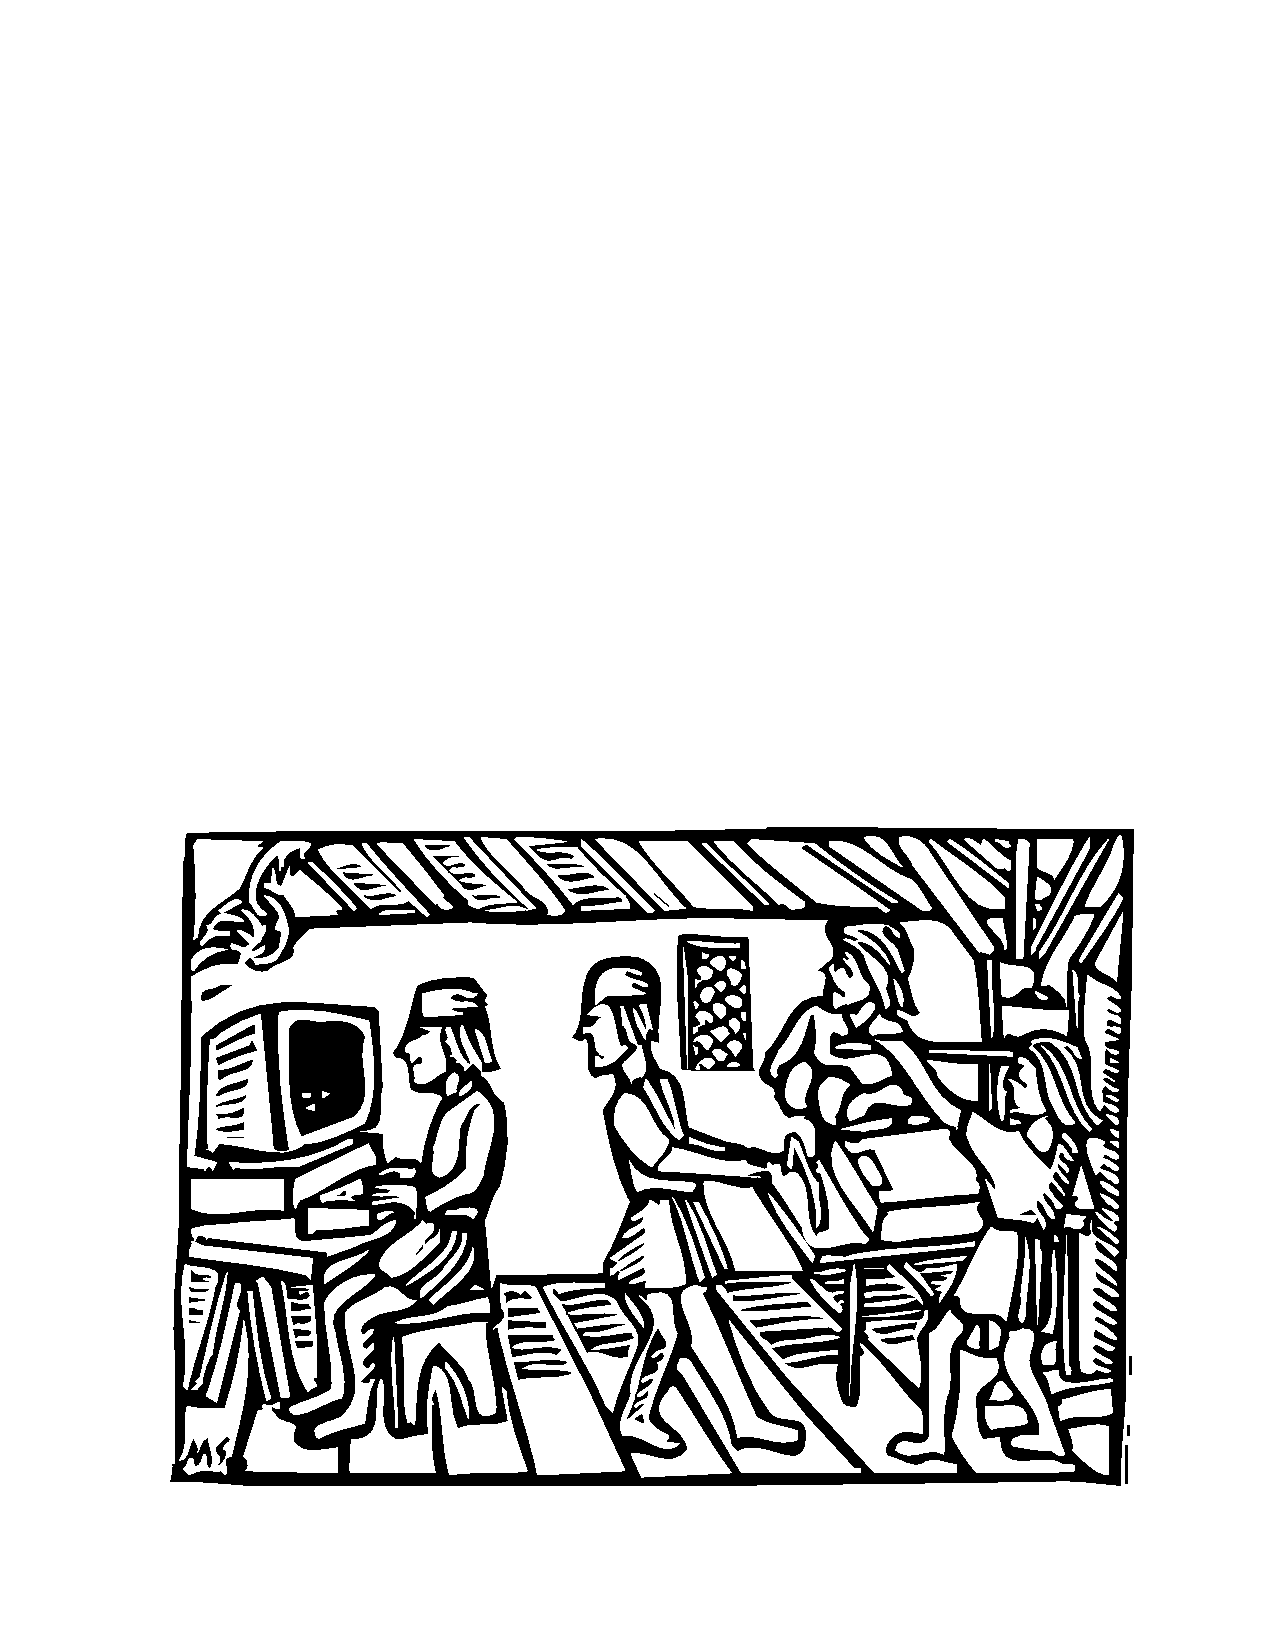
\includegraphics[width=.27\textwidth]{typography}} \qquad
\subfloat[]{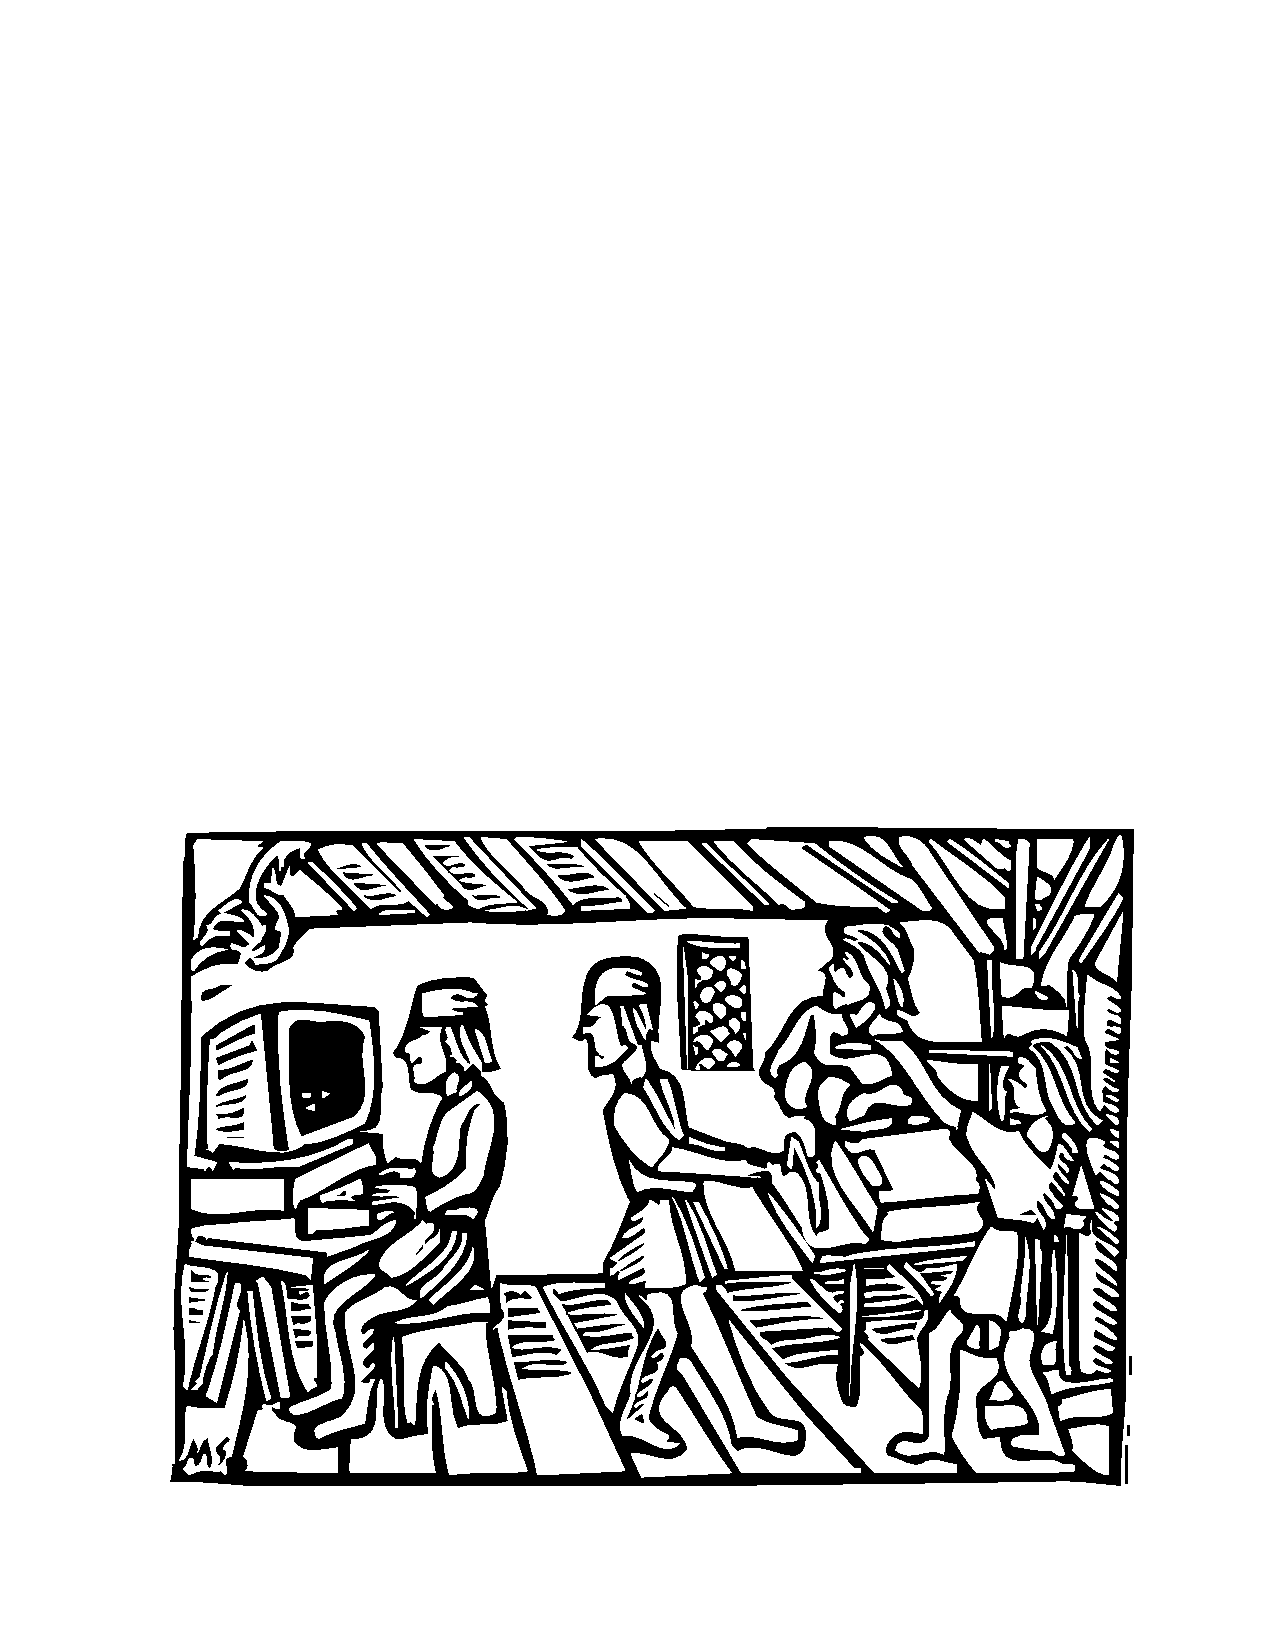
\includegraphics[width=.27\textwidth]{typography}} \qquad
\subfloat[]{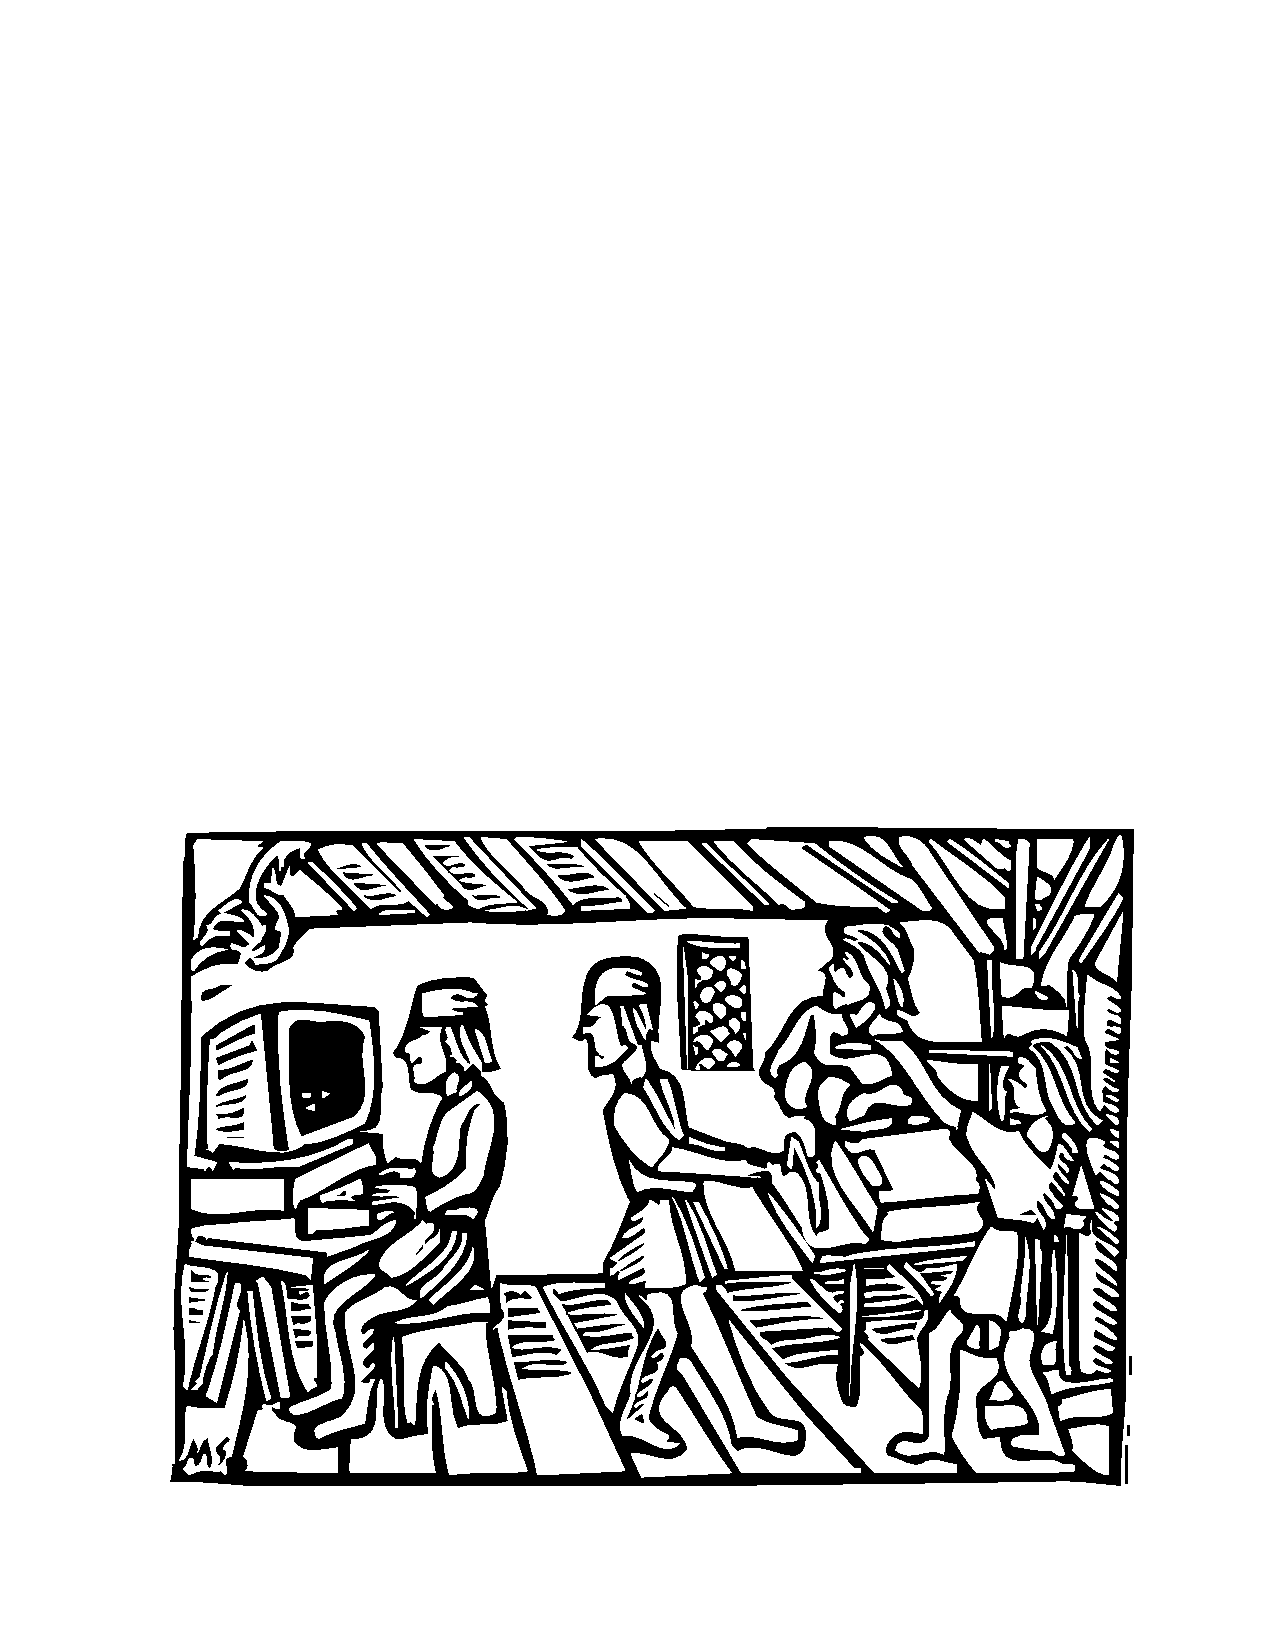
\includegraphics[width=.27\textwidth]{typography}}
\caption{并排图片}
\label{fig:subfig:3x2}
\end{figure}

要注意,\texttt{qquad}相当于\verb|\hspace{2em}|,也就是2个字符的宽度,约0.08倍页宽,
图片宽度设定为0.27倍页宽是合适的;在该环境中,尽量不要手动换行。

向前向前向前向前,华师儿女永远向前!

如果要把编号的两个图形并排,那么小页就非常有用了:
\begin{figure}[htb]
\begin{minipage}{0.48\textwidth}
  \centering
  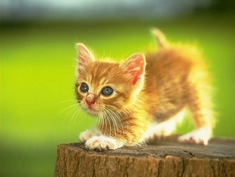
\includegraphics[height=4cm]{cat.jpg}
  \caption{并排第一个图}
  \label{fig:parallel1}
\end{minipage}\hfill
\begin{minipage}{0.48\textwidth}
  \centering
  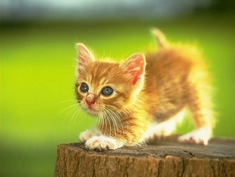
\includegraphics[height=4cm]{cat.jpg}
  \caption{并排第二个图}
  \label{fig:parallel2}
\end{minipage}
\end{figure}

\section{公式定理}
\label{sec:equation}
贝叶斯公式如式~(\ref{equ:chap1:bayes}),其中 $p(y|\mathbf{x})$ 为后验;
$p(\mathbf{x})$ 为先验;分母 $p(\mathbf{x})$ 为归一化因子。
\begin{equation}
\label{equ:chap1:bayes}
p(y|\mathbf{x}) = \frac{p(\mathbf{x},y)}{p(\mathbf{x})}=
\frac{p(\mathbf{x}|y)p(y)}{p(\mathbf{x})} 
\end{equation}

论文里面公式越多,\TeX{} 就越 happy。再看一个 \textsf{amsmath} 的例子:
\newcommand{\envert}[1]{\left\lvert#1\right\rvert} 
\begin{equation}\label{detK2}
\det\mathbf{K}(t=1,t_1,\dots,t_n)=\sum_{I\in\mathbf{n}}(-1)^{\envert{I}}
\prod_{i\in I}t_i\prod_{j\in I}(D_j+\lambda_jt_j)\det\mathbf{A}
^{(\lambda)}(\overline{I}|\overline{I})=0.
\end{equation} 

大家在写公式的时候一定要好好看 \textsf{amsmath} 的文档,并参考模板中的用法:
\begin{multline*}%\tag{[b]} % 这个出现在索引中的
\int_a^b\biggl\{\int_a^b[f(x)^2g(y)^2+f(y)^2g(x)^2]
 -2f(x)g(x)f(y)g(y)\,dx\biggr\}\,dy \\
 =\int_a^b\biggl\{g(y)^2\int_a^bf^2+f(y)^2
  \int_a^b g^2-2f(y)g(y)\int_a^b fg\biggr\}\,dy
\end{multline*}

多列公式也是比较常见的情况,比较常用的办法是用align环境实现:

\begin{equation} 
\mathbf{X} = \left(\begin{array}{ccc} 
x_{11} & x_{12} & \ldots \\ 
x_{21} & x_{22} & \ldots \\ 
\vdots & \vdots & \ddots \end{array} \right) 
\end{equation} 

\begin{equation} 
y = \left\{ \begin{array}{ll} 
a & \textrm{if $d>c$}\\ 
b+x & \textrm{in the morning}\\ 
l & \textrm{all day long} 
\end{array} \right. 
\end{equation} 

\begin{equation} 
\left(\begin{array}{c|c} 
1 & 2 \\ 
\hline 3 & 4 \end{array}\right) 
\end{equation}   

\begin{eqnarray}
f(x) & = & \cos x \\ 
f'(x) & = & -\sin x \\ 
\int_{0}^{x} f(y)\,dy & = & \sin x 
\end{eqnarray} 

{\setlength\arraycolsep{2pt} 
\begin{eqnarray} 
\sin x & = & x -\frac{x^{3}}{3!} +\frac{x^{5}}{5!}-{} \nonumber\\ 
	& & {}-\frac{x^{7}}{7!}+{}\cdots 
\end{eqnarray}} 

另外,\texttt{split}环境可能在XeCJK上不能使用,我们测试一下,看\ref{equ:split}:
\begin{equation}\label{equ:split}
\begin{split}
[z^n]C(z) &= [z^n] \biggl[\frac{e^{3/4}}{\sqrt{1-z}} +
e^{-3/4}(1-z)^{1/2} + \frac{e^{-3/4}}{4}(1-z)^{3/2}
+ O\Bigl( (1-z)^{5/2}\Bigr)\biggr] \\
&= \frac{e^{-3/4}}{\sqrt{\pi n}} - \frac{5e^{-3/4}}{8\sqrt{\pi
n^3}} + \frac{e^{-3/4}}{128 \sqrt{\pi n^5}} +
O\biggl(\frac{1}{\sqrt{\pi
n^7}}\biggr)
\end{split}
\end{equation}
\textbf{注意:} 论文模板中为了与xeCJK稳定版本兼容,调校了split命令,代价是不能在inline使用split命令。

\begin{theorem}
  \label{chapTSthm:rayleigh solution}
  假定 $X$ 的二阶矩存在:
  \begin{equation}
         O_R(\textbf{x},F)=\sqrt{\frac{\textbf{u}_1^T\textbf{A}\textbf{u}_1} {\textbf{u}_1^T\textbf{B}\textbf{u}_1}}=\sqrt{\lambda_1},
  \end{equation}
  其中 $\textbf{A}$ 等于 $(\textbf{x}-EX)(\textbf{x}-EX)^T$,\textbf{B} 表示协方差阵 $E(X-EX)(X-EX)^T$,$\lambda_1$
$\textbf{u}_1$ 是 $\lambda_1$对应的特征向量, $\omega,\ve{\omega},\omegaup,\ve{\omegaup}$.
\end{theorem}

\begin{proof}
 上述优化问题显然是一个 Rayleigh 商问题。我们有
  \begin{align}
     O_R(\textbf{x},F)=\sqrt{\frac{\textbf{u}_1^T\textbf{A}\textbf{u}_1} {\textbf{u}_1^T\textbf{B}\textbf{u}_1}}=\sqrt{\lambda_1},
 \end{align}
 其中 $\lambda_1$ 下列广义特征值问题的最大特征值:
$$
\textbf{A}\textbf{z}=\lambda\textbf{B}\textbf{z}, \textbf{z}\neq 0.
$$
 $\textbf{u}_1$ 是 $\lambda_1$对应的特征向量。结论成立。
\end{proof}

\subsection{非回路故障的推理算法}
我们知道,故障诊断的最终目的,是将故障定位到部件,而由于信号-部件依赖矩阵的存在,因此,实质性的工作是找出由故障部件发出异常信号,
不妨称为源异常信号,而如前所述,源异常信号与异常信号依赖矩阵$\mathbf{S_a}$的全零列是存在一一对应的关系的。因此,我们只要获得了$\mathbf{S_a}$的全零列的相关信息,
也就获得了源异常信号的信息,从而能进一步找到故障源。
通过以上分析,我们构造算法\ref{alg53},用于实现非回路故障诊断。

算法\ref{alg53}中,称$\beta$为源异常信号向量,该向量中与源异常信号对应的元素值为1,其它为0;
称$\gamma$为部件状态向量,该向量中非0元素对应的部件为故障部件~,0元素对应的部件为正常部件。
值得一提的是$\beta$和$\beta_a$的区别。$\beta$指出了源异常信号在所有信号中排序的位置,因此其维数与信号总数相同;
而$\beta_a$指出了源异常信号在所有异常信号中排序的位置,因此其维数与异常信号总数相同。如前所述,信号的“排序”是固定的,
这保证了算法在执行中不出现混乱。
\begin{algorithm}[htbp]
  \caption{非回路故障诊断算法}
  \label{alg53}
  \begin{algorithmic}[1]
    \REQUIRE 信号--部件依赖矩阵$\mathbf{A}$,信号依赖矩阵$\mathbf{S}$,信号状态向量$\alpha$
    \ENSURE 部件状态向量$\gamma$
    \STATE $\mathbf{P}\leftarrow\left(<\alpha>\right)$
    \STATE $\mathbf{S_{a}}\leftarrow\mathbf{P^T}\mathbf{S}\mathbf{P}$
    \FOR{$i=1$ to $S_a$的阶数$m$}
    \STATE $s_i\leftarrow s_i$的第$i$个行向量
    \ENDFOR
    \STATE $\beta_a\leftarrow\lnot \left(s_1\lor s_2\lor \cdots\lor s_m\right)^T$
    \STATE $\beta\leftarrow\mathbf{P}\beta_a$
    \STATE $\gamma\leftarrow\mathbf{A}\beta$
  \end{algorithmic}
\end{algorithm}
\subsubsection{第一类故障回路的推理算法}
第一类故障回路推理与非回路故障推理是算法基本相同,稍微不同的是$\beta_a$的计算。因为第一类故障回路中的信号全部可能是源异常信号,因此我们不必计算
$\beta_a=\lnot \left(\left[s_1\lor s_2\lor \cdots\lor s_m\right]^T\right)$,而直接取$\beta_a=\underbrace{\left[\begin{array}{cccc}1&1&\cdots&1\end{array}\right]^T}_m$,将$\beta_a$代入
算法\ref{alg53},有
\[\beta=\mathbf{P}\beta_a=\mathbf{P}\underbrace{\left[\begin{array}{cccc}1&1&\cdots&1\end{array}\right]^T}_m=\alpha\]
因此一类故障回路的推理算法变得相当简单,例如算法\ref{alg54}
\begin{algorithm}[htbp]
  \caption{第一类故障回路诊断算法}
  \label{alg54}
  \begin{algorithmic}[1]
    \REQUIRE 信号--部件依赖矩阵$\mathbf{A}$,信号状态向量$\alpha$
    \ENSURE 部件状态向量$\gamma$
    \STATE $\gamma\leftarrow\mathbf{A}\alpha$
  \end{algorithmic}
\end{algorithm}

\section{参考文献}
\label{sec:bib}
当然参考文献可以直接写 bibitem,虽然费点功夫,但是好控制,各种格式可以自己随意改
写,在\scnuthesis{}里面,建议使用JabRef编辑和管理文献,再结合\verb|bstutf8.bst|之后,
对中文的支持也很好。

本模板推荐使用 BIB\TeX,样式文件为 bstutf8.bst,基本符合学校的参考文献格式(如专利
等引用未加详细测试)。看看这个例子,关于书的\upcite{tex, companion},
还有这些\upcite{clzs},关于杂志的\upcite{ELIDRISSI94,
  MELLINGER96, SHELL02},硕士论文\upcite{zhubajie, metamori2004},博士论文
\upcite{shaheshang, FistSystem01},标准文件\upcite{IEEE-1363}~,会议论文\upcite{DPMG},%
技术报告\upcite{NPB2}。中文参考文献\upcite{cnarticle}\textsf{特别注意},需要在\verb|bibitem|中
增加\verb|language|域并设为\verb|zh|,英文此项可不填,之后由\verb|bstutf8|统一处理
(具体就是决定一些文献的显示格式,如等、etc)。
若使用\verb|JabRef|,则选择\textsf{Options}$\rightarrow$\textsf{Set Up General Fields},
在\verb|General:|后加入\verb|language|就可以了。

有时候不想要上标,那么可以这样 \cite{shaheshang},这个非常重要。

\section{代码高亮}
有些时候我们需要在论文中引入一段代码,用来衬托正文的内容,或者体现关键思路的实现。
在模板中,统一使用\texttt{listings}宏包,并且设置了基本的内容格式,并建议用户只
使用三个接口,分别控制:编程语言,行号以及边框。简洁达意即可,下面分别举例说明。

首先是设定语言,来一个C的,使用的是默认设置:
\begin{lstlisting}[language=C]
void sort(int arr[], int beg, int end)
{
  if (end > beg + 1)
  {
    int piv = arr[beg], l = beg + 1, r = end;
    while (l < r)
    {
      if (arr[l] <= piv)
        l++;
      else
        swap(&arr[l], &arr[--r]);
    }
    swap(&arr[--l], &arr[beg]);
    sort(arr, beg, l);
    sort(arr, r, end);
  }
}
\end{lstlisting}

当我们需要高亮Java代码,不需要行号,不需要边框时,可以:
\begin{lstlisting}[language=Java,numbers=none,frame=none]
// A program to display the message
// "Hello World!" on standard output

public class HelloWorld {
 
   public static void main(String[] args) {
      System.out.println("Hello World!");
   }
      
}   // end of class HelloWorld
\end{lstlisting}

细心的用户可能发现,行号被放在了正文框之外,事实上这样是比较美观的,如果有些用户希望在正文框架之内布置所有内容,
可以:
\begin{lstlisting}[language=perl,xleftmargin=2em,framexleftmargin=1.5em]
#!/usr/bin/perl
print "Hello, world!\n";
\end{lstlisting}

好了,就这么多,\texttt{listings}宏包的功能很强大也很复杂,如果需要自己定制,可以
查看其手册,耐心阅读总会找到答案。\textbf{注意:} 当前中文注释的处理还不是很完善,
对于注释请妥善处理。在本模板中,推荐算法环境或者去掉中文的listings代码环境。如果
需要包含中文注释,不要求代码高亮~,就用\texttt{code}环境,这个环境是Verbatim的定制
版,调用的fancyvbr宏包,用户可在myscnu.sty中修改。

\begin{code}
public class HelloWorld {
   public static void main(String[] args) {
      System.out.println("Hello World!");
   }
}   // 世界,你好!
\end{code}

\section{中文习惯}
\label{sec:chinese}

对于itermize过大的行间距,用户可以使用compactitem环境来替代,但是模板中不进行默认替代,
因为只有用户真正发现列表不好看才会找到这里。

对于中文双引号,可以直接使用全角的\verb|“|和\verb|”|。但是英文则不行!英文的引
号用法请自行Google,或者阅读我的
\href{https://dl.dropbox.com/u/49734213/LaTeX%E6%9C%AD%E8%AE%B0.pdf}{\LaTeX{}}札
记。

中文破折号为一个两个字宽垂直居中的直线,输入法直接得到的破折号没有垂直居中(——),
这看起来不舒服。所以模板中定义了一个破折号的命令 \verb|\pozhehao|,请看:

艰苦奋斗、严谨治学、求实创新、为人师表\hfill \pozhehao{}华南师范大学校训
%
\chapter{绪论}
大量数据代表了价值。数据背后通常隐含着客观规律,如果数据量足够大的话,其规律是可以被认知和学习的,其催生了机器学习的研究方向,研究如何用数据进行建模与变现。然而,由于数据量极大,而且所涉及的算法会很复杂,通常不可能进行人为的计算,即使是用计算机进行计算,也对计算机的处理速度,内存,储存空间提出了一定的要求。另一方面,如若要进行机器学习,除了计算机硬件的要求之外,还需要软件与算法的支持,其中,算法是机器学习的核心。历史发展来看,计算机硬件,用于机器学习的软件与算法的发展是相辅相成的。

在20世纪40年代,人们开始研究人工智能,由于生物学的发展,人们模仿人类的神经元运作而提出了神经网络的原型:M-P神经元模型,并提出了激活函数的概念。在20世纪50年代到60年代,感知器算法、梯度下降法、最小二乘法等求解算法面世,而且提出了感知器,并开始应用在文字、语音、信号等领域。在20世纪60年代到70年代,神经网络算法因感知器的缺陷而衰落。在70年代到80年代,神经网络的种类变得丰富起来,涌现出BP神经网络,RBF神经网络等各种网络,并提出了深度学习的概念与卷积神经网络(CNN)和循环神经网络(RNN)的结构。90年代后,一些有别于神经网络的算法面世,如SVM,决策树,boosting与随机森林等方法,从不同的角度对机器学习算法进行丰富。在2006年,Hinton提出了解决深度学习中梯度消失问题的解决方法之后,深度学习开始爆发。2012年,ReLU激活函数的提出,进一步抑制了梯度消失的问题,并且深度学习在语音和图像方面开始有惊人的表现。2012年,在ImageNet图像识别比赛上,AlexNet通过构建一定深度的CNN夺得冠军,其性能彻底击败了SVM。需注意的是,AlexNet首次使用了ReLU激活函数,Dropout防止过拟合方法,以及GPU加速。之后,在AlexNet的结构上做优化,又提出了其他更强大的模型,如VGGNet,Inception系列,ResNet等。强化学习和迁移学习的提出,进一步增强了模型的性能。

本论文基于kaggle(全球数据科学平台)的花苗分类竞赛(Plant Seedlings Classification\footnote{\url{https://www.kaggle.com/c/plant-seedlings-classification}})中的数据集,探究传统机器学习算法(SVM,决策树,随机森林与boosting等)、深度学习算法(AlexNet,VGGNet,InceptionV3)的原理与性能,并对其尝试做优化与结合(如AlexNet+SVM等)。

\chapter{论文正文}
\section{花苗分类问题}
该问题来自于kaggle的Plant Seedlings Classification竞赛。给定的13类花苗(有枝干,树叶,无花)的四千余张彩色图片用于训练、构建模型。其数据基本情况如表~\ref{table:sjjb}

\begin{table}[htbp]
\centering
\caption{数据基本情况}
\begin{tabular}{ccc}
\toprule[2pt]
序号 & 种类 & 样本数量 \\ 
\midrule[1pt]
1 & Black-grass & 263 \\ 
2 & Charlock & 390 \\ 
3 & Cleavers & 287 \\ 
4 & Common Chickweed & 611 \\ 
5 & Common wheat & 221 \\ 
6 & Fat Hen & 475 \\ 
7 & Loose Silky-bent & 654 \\ 
8 & Maize & 221 \\  
9 & Scentless Mayweed & 516 \\ 
10 & Shepherds Purse & 231 \\ 
11 & Small-flowered Cranesbill & 496 \\ 
12 & Sugar beet & 385 \\ 
\midrule[1pt]
总和 & -- & 4750\\
\bottomrule[2pt]
\end{tabular} 
\label{table:sjjb} 
\end{table}


而且每一张的图片大小都有可能不同。每一类的图像的例子如图~\ref{fig:myl1},~\ref{fig:myl2},~\ref{fig:myl3},~\ref{fig:myl4}
\begin{figure}[htbp]
\centering
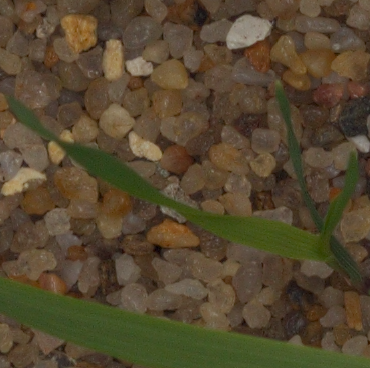
\includegraphics[width=30mm,height=30mm]{../figures/Black-grass_1af1eddd3.png} 
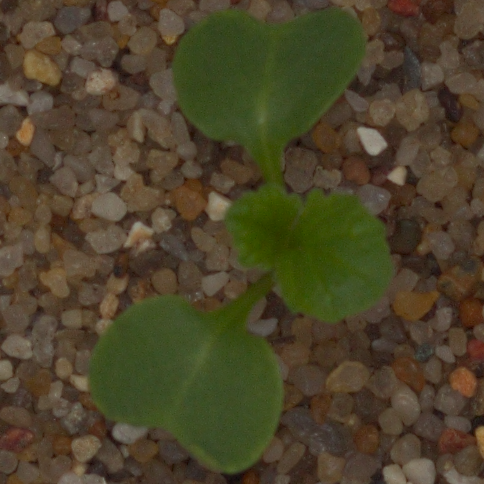
\includegraphics[width=30mm,height=30mm]{../figures/Charlock_0a7e1ca41.png} 	
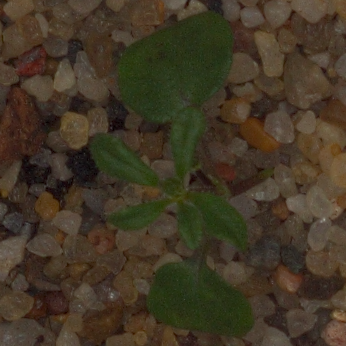
\includegraphics[width=30mm,height=30mm]{../figures/Cleavers_0a1e622bc.png} 	
\caption{从左到右分别为Black-grass,Charlock,Cleavers的一张图片,像素分别为$370\times368$,$484\times484$,$346\times346$}
\label{fig:myl1}
\end{figure}

\begin{figure}[htbp]
\centering
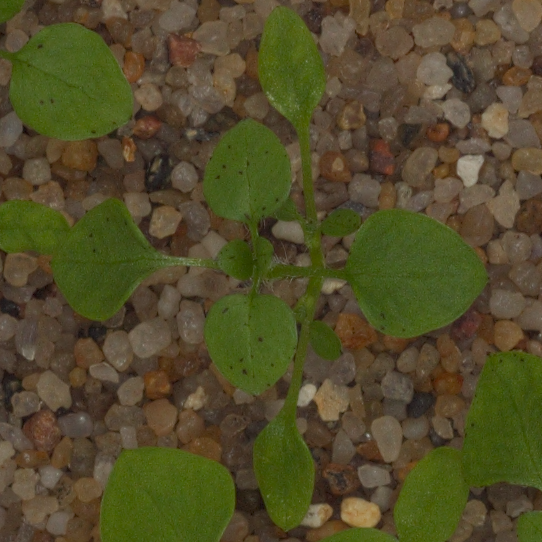
\includegraphics[width=30mm,height=30mm]{../figures/Common_Chickweed_0a1c68ef9.png} 	
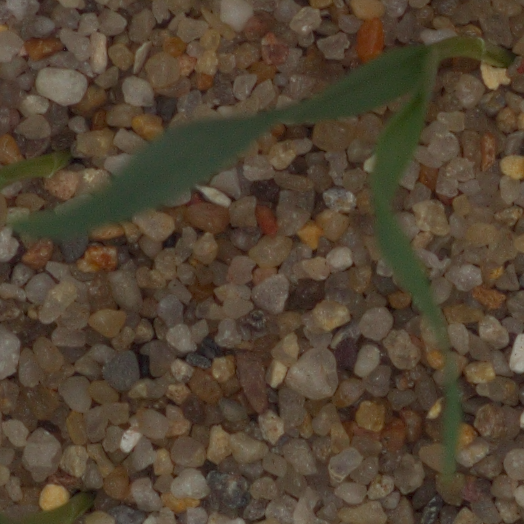
\includegraphics[width=30mm,height=30mm]{../figures/Common_wheat_6dfb9a152.png} 	
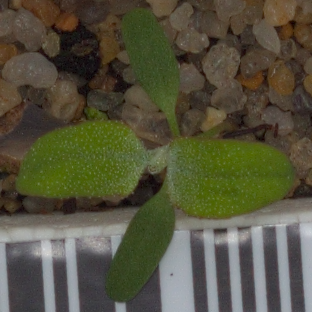
\includegraphics[width=30mm,height=30mm]{../figures/Fat_Hen_0eeb0c7c1.png}	
\caption{从左到右分别为Common Chickweed,Common wheat,Fat Hen的一张图片,像素分别为$542\times542$,$524\times524$,$312\times312$}
\label{fig:myl2}
\end{figure}

\begin{figure}[htbp]
\centering
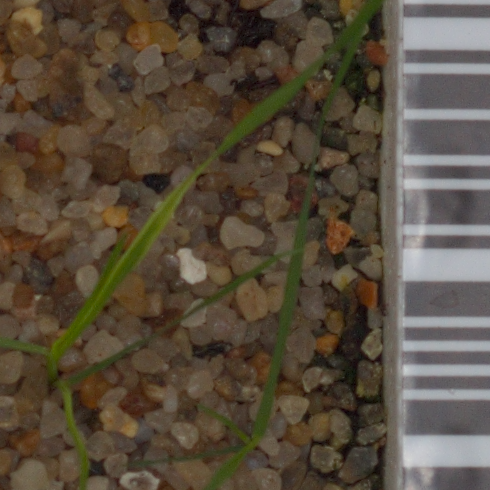
\includegraphics[width=30mm,height=30mm]{../figures/Loose_Silky-bent_3cac767c2.png} 	
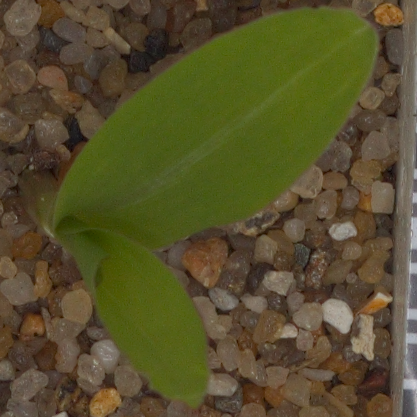
\includegraphics[width=30mm,height=30mm]{../figures/Maize_1d21b25f9.png}	
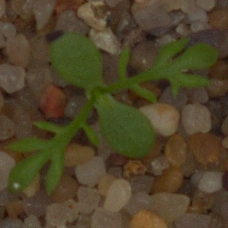
\includegraphics[width=30mm,height=30mm]{../figures/Scentless_Mayweed_0ae9acf83.png}
\caption{从左到右分别为Loose Silky-bent,Maize,Scentless Mayweed的一张图片,像素分别为$490\times490$,$417\times417$,$228\times228$}
\label{fig:myl3}
\end{figure}

\begin{figure}[htbp]
\centering
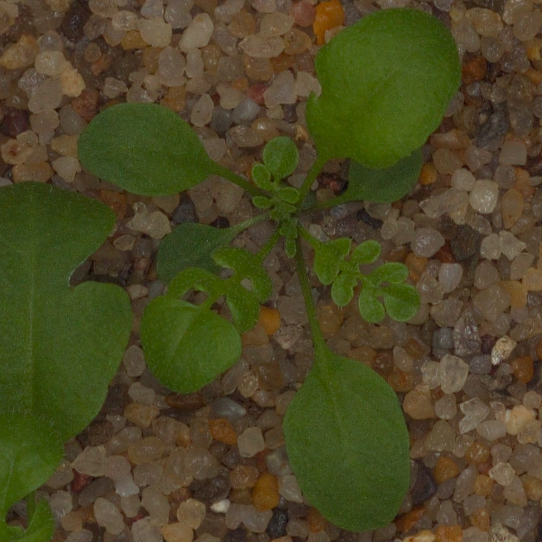
\includegraphics[width=30mm,height=30mm]{../figures/Shepherds_Purse_0bef4ae08.png} 	
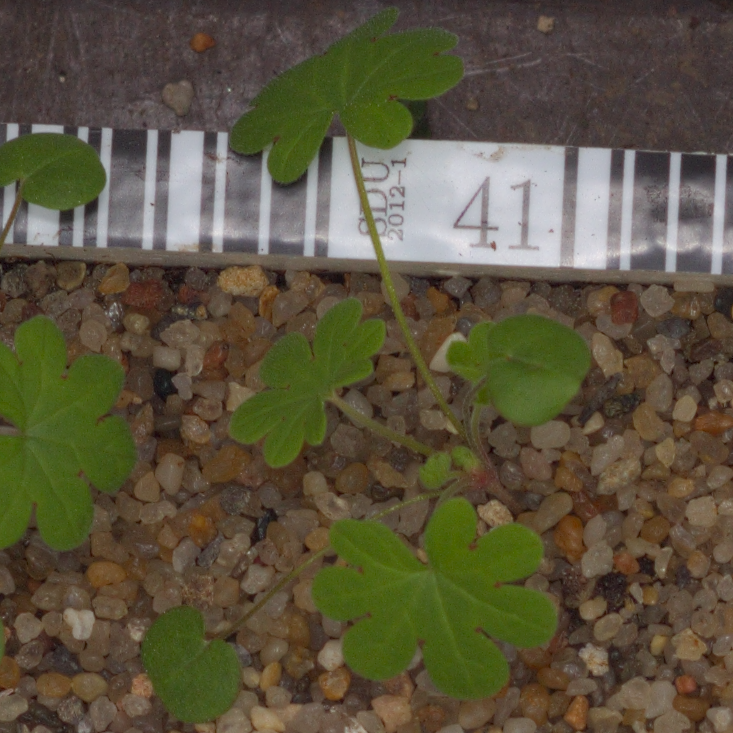
\includegraphics[width=30mm,height=30mm]{../figures/Small-flowered_Cranesbill_0e7f05ec0.png} 	
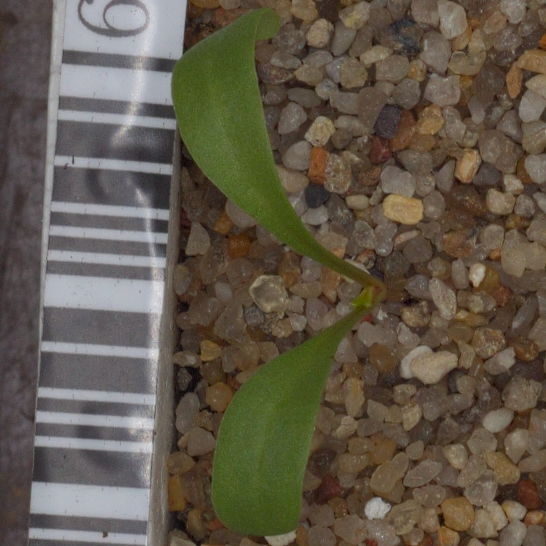
\includegraphics[width=30mm,height=30mm]{../figures/Sugar_beet_1bdfd2206.png}
\caption{从左到右分别Shepherds Purse,Small-flowered Cranesbill,Sugar beet的一张图片,像素分别为$542\times542$,$733\times733$,$546\times546$}
\label{fig:myl4}
\end{figure}

由于所涉及到的数据为彩色图像,而花苗的特征为绿色,故考虑使用opencv的方法,通过建立掩膜筛选出花苗的图像,进而将彩色图像转化为灰度图像或二值图像,从而达到降维的目的。而即使降维之后,为了确保图像失真不大,所以至少将图像转化为$64\times 64$的灰度图像矩阵。若考虑直接采用Logistic、SVM或决策树方法,则需要将$64\times 64$的灰度图像矩阵拉伸为$4096\times 1$的图像,然而假设用全部的数据进行训练,也只有4750个样本,训练时极容易导致过拟合,但是,考虑集成学习的方法或是带dropout的BP神经网络可以一定程度上防止过拟合。考虑到为涉及图像的分类问题,可以采用卷积神经网络(CNN)。由于是13类的分类问题,且样本数较少,可以进一步考虑在用SVM、Logistic或决策树方法来替代神经网络最后的softmax层,或许能起到更好的效果。
\section{数据预处理}
\subsection{掩模构建与形态学去噪}
对于花苗图像,我们可以看到,花苗的背景通常为黄土、砂砾或塑料箱等,而绿色的花苗则显得非常好辨认。而且我们面对的花苗是绿色的,因而考虑设置一个hsv范围,将绿色的部分从图像中剥离出来。于是我们首先将花苗图像进行颜色空间的转换,从rgb颜色空间转化为hsv颜色空间,之后设定hsv颜色空间为[26,43,46]和[99,255,255],在原图中过滤出在这个hsv颜色空间的图像得到掩膜,若在这个区间中,则为白色,否则为黑色。之后可以通过该掩膜对原图进行位运算,则可得到原图的图像。其部分代码如下
\begin{lstlisting}[language=python]
import cv2
# 假设待处理的图像为img
# rgb图像转化为hsv图像
hsv = hsv = cv2.cvtColor(img,cv2.COLOR_BGR2HLS)
# 绿色的阈值(HSV)
lower_green = np.array([26,43,46])
upper_green = np.array([99,255,255])
# 根据阈值构建掩膜
mask = cv2.inRange(hsv,lower_green,upper_green)
# 对原图像和掩膜进行位运算
res = cv2.bitwise_and(img,img,mask=mask)
\end{lstlisting}
得到的结果如下,以Black-grass,Charlock,Cleavers种类的各一个图像为例,如图~\ref{fig:bg1},~\ref{fig:ch1},~\ref{fig:ch1},~\ref{fig:cl}

\begin{figure}[htbp]
\centering
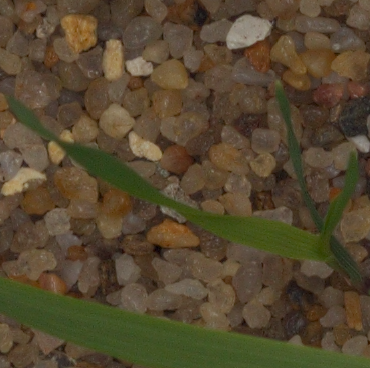
\includegraphics[width=30mm,height=30mm]{../figures/Black-grass_1af1eddd3.png} 
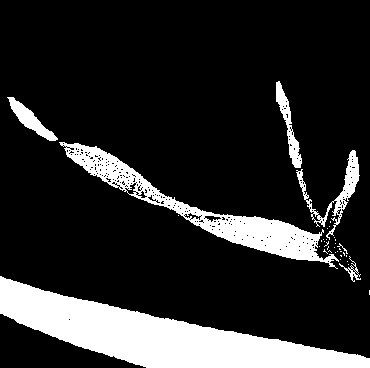
\includegraphics[width=30mm,height=30mm]{../figures/Black-grass_1af1eddd3_mask.png} 	
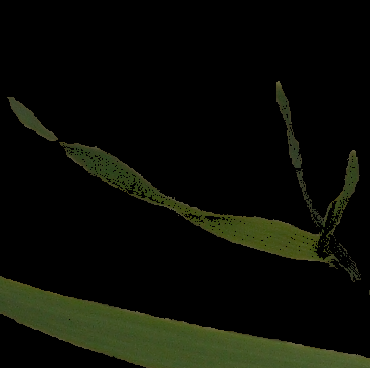
\includegraphics[width=30mm,height=30mm]{../figures/Black-grass_1af1eddd3_res.png} 
\caption{Black-grass的一个图像,其大小为$370\times 368$,从左到有依次为原图,掩膜图像,通过掩膜对原图过滤的图像}
\label{fig:bg1} 
\end{figure}

\begin{figure}[htbp]
\centering
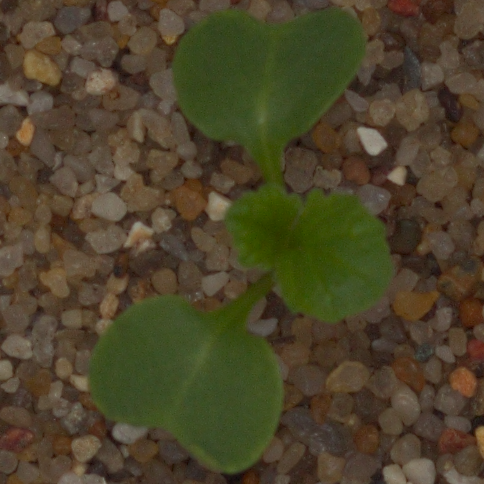
\includegraphics[width=30mm,height=30mm]{../figures/Charlock_0a7e1ca41.png} 
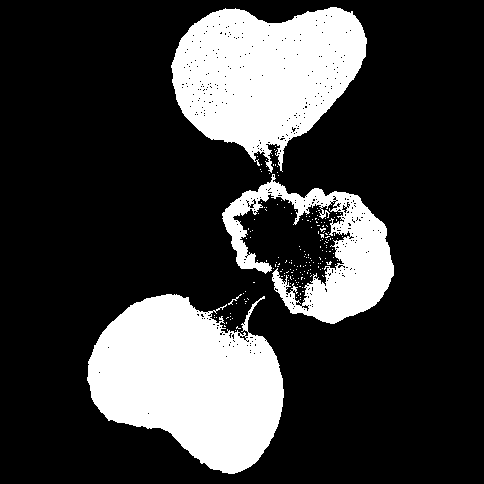
\includegraphics[width=30mm,height=30mm]{../figures/Charlock_0a7e1ca41_mask.png} 	
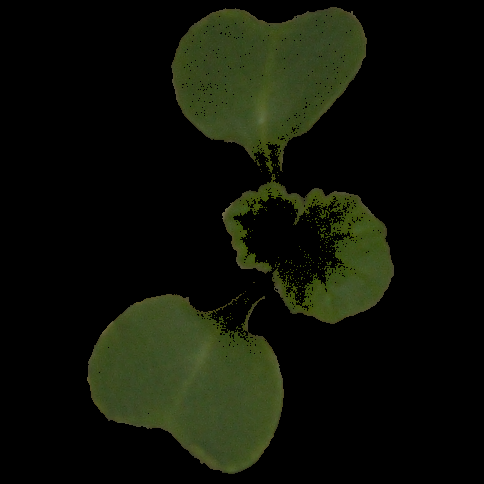
\includegraphics[width=30mm,height=30mm]{../figures/Charlock_0a7e1ca41_res.png} 	
\caption{Charlock的一个图像,其大小为$484\times 484$,从左到有依次为原图,掩膜图像,通过掩膜对原图过滤的图像}
\label{fig:ch1} 
\end{figure}

\begin{figure}[htbp]
\centering
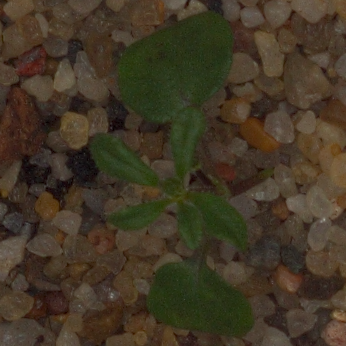
\includegraphics[width=30mm,height=30mm]{../figures/Cleavers_0a1e622bc.png} 
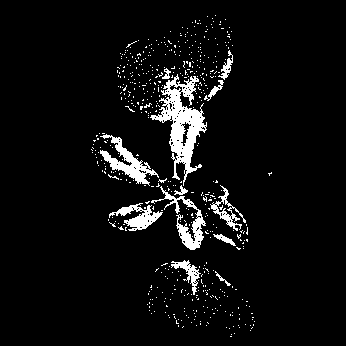
\includegraphics[width=30mm,height=30mm]{../figures/Cleavers_0a1e622bc_mask.png} 	
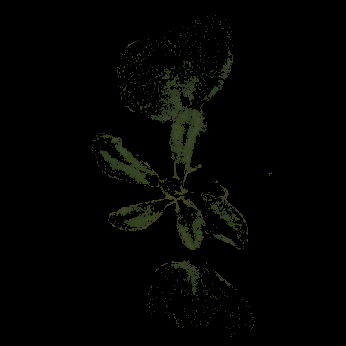
\includegraphics[width=30mm,height=30mm]{../figures/Cleavers_0a1e622bc_res.png} 
\caption{Cleavers的一个图像,其大小为$346\times 346$,从左到有依次为原图,掩膜图像,通过掩膜对原图过滤的图像}
\label{fig:cl} 
\end{figure}



\subsection{形态学去噪}
对于用掩模处理后的花苗二值图像,考虑到在花苗所在盆栽可能会有一些小草,通过掩模处理后会有噪声。因而考虑用形态学方法去噪。

对于一个二值图像,比较常用的去噪方法是形态学去噪,而这通常涉及两种形态学转换,分别为腐蚀和膨胀,其涉及的原理较简单。对于腐蚀,先定义一个窗口,窗口将沿着图像滑动,以遍历整个图像。滑动过程中,窗口内所有像素不全为1时,则令窗口中的所有像素等于0;若窗口内所有像素全为1,时,则不做操作。选用一个合适尺寸的窗口,对于腐蚀之后的图片,其白噪声点可以消除,但也会对物体的边缘进行腐蚀。膨胀则与腐蚀相反,区别在于滑动过程中,窗口内元素只要有1,则整个窗口元素都令为1,这样会增大物体的尺寸。通常对于有白噪声的图片,先腐蚀再膨胀可以消除白噪声,但一定程度会导致物体失真。但由于用掩模处理后的图像,其物体十分明显,用形态学方法去噪后失真的可能性不大。因而考虑用形态学方法去噪。
\subsection{边框裁剪与尺寸统一化}
我们从掩膜图像可以看出,目标图像(白色部分)只是占所有图像的很小一部分,而其余其余部分为黑色,而这其余的部分往往是无效的。现在考虑用一个矩形边框去提取出图像的有效区域,而将无效区域剔除。方法是访问图像中有效区域的宽度最小值和最大值,以及高度最小值和最大值,从而确定矩形边框区域。其效果图~\ref{fig:bycj}所示
\begin{figure}[htbp]
\centering
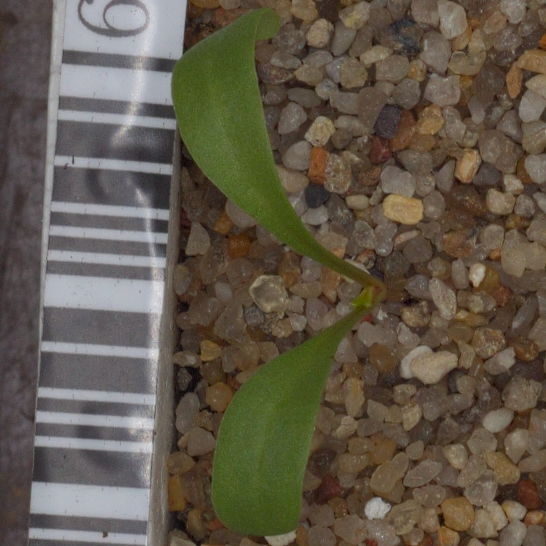
\includegraphics[width=30mm,height=30mm]{../figures/Sugar_beet_1bdfd2206.png} 

\includegraphics[width=30mm,height=30mm]{../figures/Sugar_beet_1bdfd2206_mask.png} 	

\includegraphics[width=10mm,height=30mm]{../figures/Sugar_beet_1bdfd2206_mask_tg.png}
\caption{Sugar beet的一个图像,其大小为$546\times 546$,从左到有依次为原图,掩膜图像,对掩膜图像矩形裁剪之后的图像,其大小为$199\times 530$}
\label{fig:bycj} 
\end{figure}

实现这个效果的代码如下
\begin{lstlisting}[language=python]
import cv2
# 获得矩形边框的最小宽高以及宽度和高度
x,y,w,h = cv2.boundingRect(mask_temp)
# 在原掩膜图像中选取矩形边框
mask_tg = mask[y:(y+h),x:(x+w)]
\end{lstlisting}
由于卷积神经网络需要同样大小尺寸的输入,所以考虑将图像统一尺寸归一化为统一的大小。内插的方法是INTER-CUBIC,其结果如图~\ref{fig:gyhW}

\begin{figure}[htbp]
\centering 

\includegraphics[width=10mm,height=30mm]{../figures/Sugar_beet_1bdfd2206_mask_tg.png} 	

\includegraphics[width=30mm,height=30mm]{../figures/Sugar_beet_1bdfd2206_mask_tg.png} 	\\
\caption{Sugar beet的一个图像,左边为矩形裁剪之后的图像,大小为$199\times 530$,右边为尺寸统一化后的图像,大小为$96\times 96$}
\label{fig:gyh}
\end{figure}

实现这个效果的代码如下
\begin{lstlisting}[language=python]
import cv2
# 尺寸变换
mask_tg_rs = cv2.resize(mask_tg,[96,96],interpolation=cv2.INTER_CUBIC)
\end{lstlisting}
最后,对所有的图片都做上述操作。每张图片的掩膜的尺寸归一后的图像作为输入,需要注意的是,图片格式为uint8,需要转化为float才不会出问题,用以下代码可以解决该问题。
\begin{lstlisting}[language=python]
from skimage import img_as_float
imginput = img_as_float(mask_tg_rs) 
\end{lstlisting}

制作训练模型所需的数据集时,对原有的图片输入,通过以上变换之后所得到的imginput作为数据集的输入,而对原有的图片的名字进行one-hot编码处理作为数据集的输出。采用自助法分割训练集和验证集。训练集和验证集的样本数量比为$7:3$。在制备数据集输入时,制备三种规格分别为$64\times64$,$96\times96$,$128\times128$的数据集输入,而数据集输出不变,以探究不同大小的图片输入对神经网络性能的影响。为了方便表示,将上面三种规格的数据分别命名为I64,I96,I128,如表~\ref{table:t0}所示



\begin{table}[htbp]
\centering
\caption{训练集与验证集的构成}
\label{table:t0} 
\begin{tabular}{cccc}
\toprule[2pt] 
数据集名称 & 数据集用途 & 输入的数据特征 & 输出的数据特征 \\ 
\midrule[2pt]
\multirow{2}{*}{I64} & 训练集 & $3325,64,64,1$ & $3325,10$ \\ 
 & 验证集 & $1425,64,64,1$ & $1425,10$ \\ 
\midrule[1pt]
\multirow{2}{*}{I96} & 训练集 & $3325,96,96,1$ & $3325,10$ \\ 
 & 验证集 & $1425,96,96,1$ & $1425,10$ \\ 
\midrule[1pt]
\multirow{2}{*}{I128} & 训练集 & $3325,128,128,1$ & $3325,10$ \\ 
 & 验证集 & $1425,128,128,1$ & $1425,10$ \\ 
\bottomrule[2pt]
\end{tabular} 
\end{table}




\section{BP神经网络与卷积神经网络}
\subsection{神经网络的构造与前向传播}
神经网络是由单个或多个神经元组成。下图~\ref{fig:bp1}是单个神经元的构造。
\begin{figure}[htb]
\centering
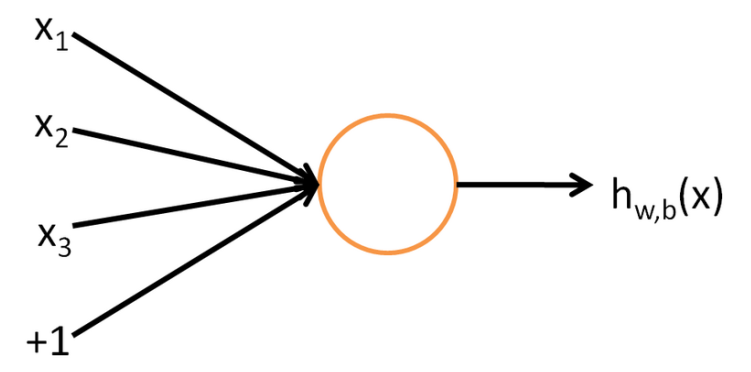
\includegraphics[scale=0.5]{../figures/NN1.png}
\caption{神经元}
\label{fig:bp1}
\end{figure}



该神经元的输入由三个数据$x_1,x_2,x_3$以及偏置项(bias)+1组成,通过神经元后输出的表达式为
\begin{eqnarray}
h_{W,b}(x)=f(W^Tx+b)=f(\sum_{i=1}^3 W_ix_i+b)
\end{eqnarray}
其中$f$为激活函数。激活函数是为了将线性项$W^Tx$变换为非线性。在BP中,较常用的激活函数为sigmoid函数,其表达式如下
\begin{eqnarray}
f(z)=\frac{1}{1+\exp(-z)}
\end{eqnarray}
另外,令$b=w_0$,则可重新定义$W=(w_0,w_1,w_2,w_3)^T$,$x=(1,x_1,x_2,x_3)$,于是可将上式写为
\begin{eqnarray}
h_{W,b}(x)=f(W^Tx)
\end{eqnarray}
下面讨论神经网络。多个神经元可以组成一个层,多个层互相连接可以组成神经网络。其中,接受数据输入的层为输入层,数据计算后的数据的输出层,中间的层则称为隐含层。下图~\ref{fig:bp2}是含有两个隐含层的神经网络。
\begin{figure}[htb]
\centering
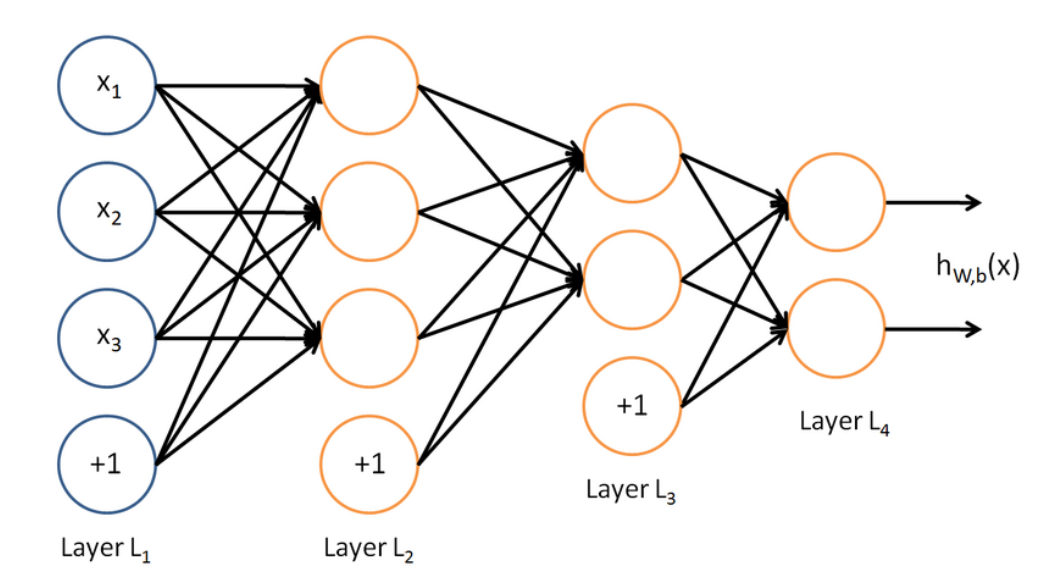
\includegraphics[scale=0.5]{../figures/NN2.png}
\caption{含有两个隐含层的神经网络}
\label{fig:bp2}
\end{figure}
如图,最左边的为输入层,即图中的Layer L1,最右边的为输出层,即图中的Layer L4,中间的所有层,即图中的Layer L2,Layer L3为隐含层。

我们用$n_l$来表示网络的层数,记第$i$层为$L_i$,于是输入层为$L_1$,输出层为$L_{n_l}$。由于神经网络可以有任意多的隐层以及隐藏神经元,则我们记$\samplet{W}{l}{ij}$为第$l$层第$j$单元以及第$l+1$层第$i$单元之间的连接权重,$\samplet{b}{l}{i	}$为第$L+1$层第$i$单元的偏执。我们用$\samplet{a}{l}{i}$表示第$l$层第$i$单元的激活值(输出值),则有
\begin{eqnarray}
\samplet{a}{l+1}{i}=f(\sum_{j=1}^{S_l}\samplet{W}{l}{ij}\samplet{a}{l}{j}+\samplet{b}{l}{i})
\end{eqnarray}
其中当$l=1$时,$\sample{a}{l}=x$,$x$为输入向量$(x_1,x_2,\cdots,x_{S_l})$,$S_l$指第$l$层的神经元个数,我们用$\samplet{z}{l+1}{i}$表示第$l+1$层第$i$单元输入加权和(包括偏置),即
\begin{eqnarray}
\samplet{z}{l+1}{i}=\sum_{j=1}^{S_t}\samplet{W}{l}{ij}\samplet{a}{l}{j}+\samplet{b}{l}{i}
\end{eqnarray}
则有
\begin{eqnarray}
\samplet{a}{l+1}{i}&=&f(\samplet{z}{l+1}{i})\\
h_{W,b}(x)&=&\sample{a}{n_l}=f(\sample{z}{n_l})
\end{eqnarray}
上述过程称为神经网络的前向传播。

\subsection{神经网络的反向传播}
根据上面的前向传播,我们设神经网络的各层表示为$L_1,L_2,\cdots,L_{n_l}$,其中,$L_{n_l}$为输出层,对于输出层,假设输出层输出为$t=\sample{a}{n_l}$,$y$为标签,则若为回归问题,则代价函数使用MSE,即
\begin{eqnarray}
J(W,b;x,y)=\frac{1}{2}||t-y||^2
\end{eqnarray}
接下来计算输出层的残差
\begin{eqnarray}
\begin{aligned}
\samplet{\delta}{n_l}{i}&=\frac{\partial}{\partial \samplet{z}{n_l}{i}}J(W,b;x,y)\\
&=\frac{\partial}{\partial \samplet{z}{n_l}{i}}\frac{1}{2}||y-h_{W,b}(x)||^2\\
&=\frac{\partial}{\partial \samplet{z}{n_l}{i}}\frac{1}{2}\sum_{j=1}^S{_{n_l}}(y_i-\samplet{a}{n_l}{j})^2\\
&=\frac{\partial}{\partial \samplet{z}{n_l}{i}}\frac{1}{2}\sum_{j=1}^S{_{n_l}}(y_i-f(\samplet{z}{n_l}{i}))^2\\
&=-(y_i-f(\samplet{z}{n_l}{i}))\cdot f'(\samplet{z}{n_l}{i})\\
&=-(y_i-\samplet{a}{n_l}{i})\cdot f'(\samplet{z}{n_l}{i})
\end{aligned}
\end{eqnarray}
下面考虑残差的递推算法,以输出层前一层为例。由前向传播我们可以推导出
\begin{eqnarray}
\samplet{z}{l+1}{i}=\sum_{j=1}^{S_l}\samplet{W}{l}{ij}f(\samplet{z}{l}{i})+\samplet{b}{l}{i}
\end{eqnarray}
则有
\begin{eqnarray}
\samplet{z}{n_i}{i}=\sum_{j=1}^{S_l} \samplet{W}{n_l-1}{ij}f(\samplet{z}{n_l-1}{i})+\samplet{b}{n_l-1}{i}
\end{eqnarray}
于是有
\begin{eqnarray}
\frac{\partial \samplet{z}{n_l}{i}}{\partial \samplet{z}{n_l-1}{i}}=\sum_{j=1}^{S_l}\samplet{W}{n_l-1}{ij}f'(\samplet{z}{n_l-1}{i})
\end{eqnarray}
则可以得到输出层前一层的残差
\begin{eqnarray}
\begin{aligned}
\samplet{\delta}{n_l-1}{i} &= \frac{\partial}{\partial \samplet{z}{n_l-1}{i}}J(W,b;x,y)\\
&= \frac{\partial J(W,b;x,y)}{\partial \samplet{z}{n_l}{i}}\cdot\frac{\partial \samplet{z}{n_l}{i}}{\partial \samplet{z}{n_l-1}{i}}\\
&= \sum_{j=1}^{S_l}\samplet{\delta}{n_l}{j}\samplet{W}{n_l-1}{ij}f'(\samplet{z}{n_l-1}{i})
\end{aligned}
\end{eqnarray}
将$n_l-1$与$n_l$的关系替换为$l$与$l+1$的关系,则可得到
\begin{eqnarray}
\samplet{\delta}{l}{i}=\frac{\partial}{\partial \samplet{z}{l}{i}}J(W,b;x,y)=
\left(
	\begin{aligned}
		\sum_{j=1}^{S_{l+1}}\samplet{W}{l}{ji}\samplet{\delta}{l+1}{j}
	\end{aligned}
\right)
f'(\samplet{z}{l}{i})
\end{eqnarray}
若取函数$f$为sigmoid函数,则有
\begin{eqnarray}
f'(\samplet{z}{l}{i})=f(\samplet{z}{l}{i})\circ(1-f(\samplet{z}{l}{i}))=\samplet{a}{l}{i}\circ(1-\samplet{a}{l}{i})
\end{eqnarray}
其中$\circ$代表点乘。于是可得到$\samplet{\sigma}{l+1}{j}$到$\samplet{\sigma}{l}{j}$的递推式:
\begin{eqnarray}
\samplet{\delta}{l}{i}=
\left(
	\begin{aligned}
		\sum_{j=1}^{S_{l+1}}\samplet{W}{l}{ji}\samplet{\delta}{l+1}{j}
	\end{aligned}
\right)
(\samplet{a}{l}{i}\circ(1-\samplet{a}{l}{i}))
\end{eqnarray}
反向传播,一般采用梯度下降法对每一层的权重进行调整,即
\begin{eqnarray}
\samplet{W}{l}{ij}=\samplet{W}{l}{ij}-\alpha\frac{\partial}{\partial \samplet{W}{l}{ij}}J(W,b;x,y)
\end{eqnarray}
其中,$\alpha$是学习率。因而需要求权重$\samplet{W}{l}{ij}$对于代价函数的偏导,此时可使用当前层的残差来进行计算,即
\begin{eqnarray}
\frac{\partial}{\partial \samplet{W}{l}{ij}}J(W,b;x,y)=\frac{\partial J(W,b;x,y)}{\partial \samplet{z}{l+1}{i}}\frac{\samplet{z}{l+1}{i}}{\samplet{W}{l}{ij}}
\end{eqnarray}
又有
\begin{eqnarray}
\frac{\samplet{z}{l+1}{i}}{\samplet{W}{l}{ij}}=\frac{\left( \sum_{j=1}^{S_l}\samplet{W}{l}{ij}f(\samplet{z}{l}{i}) \right)}{\samplet{W}{l}{ij}}=f(\samplet{z}{l}{i})=\samplet{a}{l}{i}
\end{eqnarray}
于是可得
\begin{eqnarray}
\frac{\partial}{\partial \samplet{W}{l}{ij}}J(W,b;x,y)=\samplet{a}{l}{j}\samplet{\delta}{l+1}{i}
\end{eqnarray}
综上,可以总结BP神经网络算法
\textbf{BP神经网络算法}

\begin{lstlisting}[language=python]
`输入:训练输入$x$,训练输出$y$,学习率$\alpha$`
while `未达到收敛条件`
    `
	输入训练输入,训练输出,学习率\\
	1.初始化神经网络的权重与偏置\\
	2.对输入进行前向传播,得到除输入层外每一层($L_2,\cdots,L_{n_l}$)的激活值$\sample{a}{2},\cdots,\sample{a}{n_l}$\\
	3.计算各层残差:\\
	(1)对输出层(第$n_l$层)
	\begin{eqnarray}
	\sample{\delta}{n_l}=-(y-\sample{a}{n_l})\cdot(\sample{a}{l}\circ(1-\sample{a}{l}))
	\end{eqnarray}
	(2)对于$l=n_l-1,\cdots,2$各层,可递推得出残差值
	\begin{eqnarray}
	\sample{\delta}{l}=((\sample{W}{l})^T\sample{\delta}{l+1})\cdot(\sample{a}{l})
	\end{eqnarray}
	(3)计算损失函数对每一层权重的偏导数值
	\begin{eqnarray}
	\nabla_{\sample{W}{l}}J(W,b;x,y)=\sample{\delta}{l+1}(\sample{a}{l})^T
	\end{eqnarray}
	(4)更新参数
	\begin{eqnarray}
	\sample{W}{l}=\sample{W}{l}-\alpha\nabla_{\sample{W}{l}}J(W,b;x,y)
	\end{eqnarray}
    `
end

\end{lstlisting}

若为多分类问题,先对$y$进行one-hot处理得到$p$维向量$(y_1,y_2,\cdots,y_p)$(假设$y$有$p$种取值),并将输出层的激活函数选为softmax,即
\begin{eqnarray}
\samplet{a}{n_l}{i}=f_s(\samplet{z}{n_l}{i})=\frac{e^{\samplet{z}{n_l}{i}}}{\sum_je^{\samplet{z}{n_l}{j}}}
\end{eqnarray}
并且代价函数使用交叉熵损失函数
\begin{eqnarray}
J(W,b;x,y)=-\sum_i y_i\log \samplet{a}{n_l}{i}
\end{eqnarray}
则输出层残差为
\begin{eqnarray}
\begin{aligned}
\samplet{\delta}{n_l}{i}&= \frac{\partial J}{\partial \samplet{z}{n_l}{i}}\\
&=\sum_i\frac{\partial J}{\samplet{a}{n_l}{i}}\cdot\frac{\partial \samplet{a}{n_l}{i}}{\partial \samplet{z}{n_l}{i}}\\
&=\sum_i\frac{\partial -\sum_i y_i\log\samplet{a}{n_l}{i}}{\samplet{a}{n_l}{i}}\cdot\frac{\partial \samplet{a}{n_l}{i}}{\partial \samplet{z}{n_l}{i}}\\
&=-\sum_i\frac{y_i}{\samplet{a}{n_l}{i}}\frac{\partial \samplet{a}{n_l}{i}}{\partial \samplet{z}{n_l}{j}}
\end{aligned}
\end{eqnarray}
当$i=j$时,记$e^{\samplet{z}{n_l}{j}}=e^A$,$\sum_{k\neq j}e^{\samplet{z}{n_l}{k}}=e^B$,显然有$e^A+e^B=\sum_ie^{\samplet{z}{n_l}{i}}$,于是
\begin{eqnarray}
\begin{aligned}
\frac{\partial \samplet{a}{n_l}{i}}{\partial \samplet{z}{n_l}{j}} &= \frac{\partial \samplet{a}{n_l}{j}}{\partial \samplet{z}{n_l}{j}}\\
&= \frac{\partial \frac{e^A}{e^A+e^B}}{\partial A}\\
&= \frac{e^A(e^B+e^A)-e^{2A}}{(e^A+e^B)^2}\\
&= \frac{e^Ae^B}{(e^A+e^B)^2}\\
&= \frac{e^A}{e^A+e^B}\frac{e^B}{e^A+e^B}\\
&= \frac{e^A}{e^A+e^B}(1-\frac{e^A}{e^A+e^B})\\
&= \samplet{a}{n_l}{j}(1-\samplet{a}{n_l}{j})
\end{aligned}
\end{eqnarray}
\subsection{激活函数}
\paragraph{sigmoid}
sigmoid函数表达式如下
\begin{eqnarray}
f(x)=\frac{1}{1+e^{-x}}
\end{eqnarray}
其图像如图~\ref{fig:bp3}所示
\begin{figure}[htb]
\centering
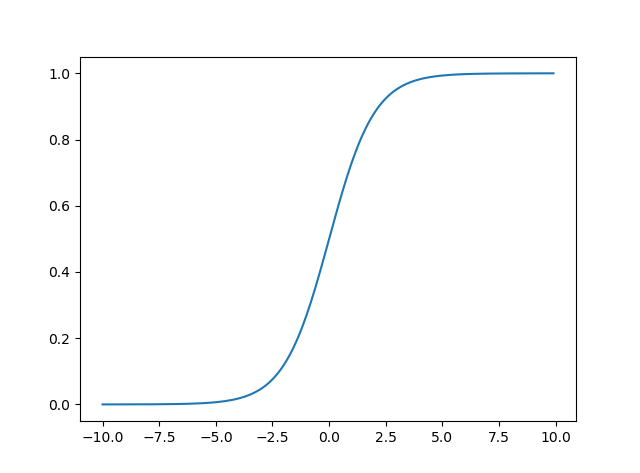
\includegraphics[scale=0.5]{../figures/NN3.png} 
\caption{sigmoid函数}
\label{fig:bp3}
\end{figure}
sigmoid激活函数考虑将输入值映射到$(0,1)$的区间中,该函数在定义域内连续,且导数大于0。它也有较为简单的求导结果
\begin{eqnarray}
f'(x)=f(x)(1-f(x))
\end{eqnarray}
但是在神经网络中,特别是对于层数较多的网络,通常不采用sigmoid作为激活函数,主要是因为其容易产生梯度消失的情况。当输入非常大或非常小的时候,其梯度趋近于0,反向传播的过程中直接导致梯度无法传播,无法有效地调整权重。虽然做标准化可以让数据近似服从正态分布,但梯度消失仍有可能产生,在学习过程中可能会产生输入较大或较小的情况。或许这个问题可以用batch-normalization来缓解,但明显采取一种更佳的激活函数是较为可取的做法。
\paragraph{ReLU}
ReLU函数表达式如下
\begin{eqnarray}
f(x)=\max\{0,x\}
\end{eqnarray}
图像如下图~\ref{fig:bp4}
\begin{figure}[htb]
\centering
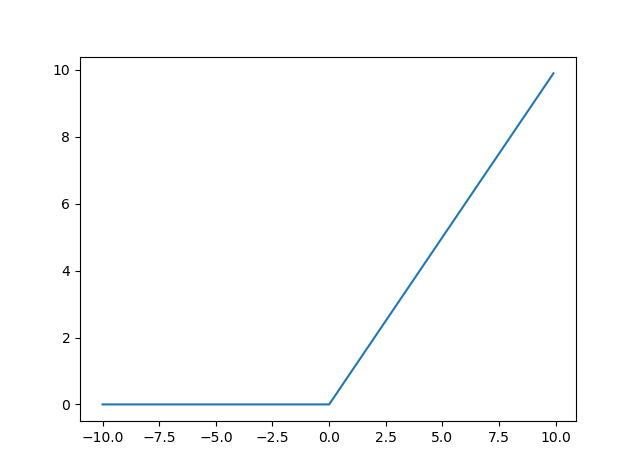
\includegraphics[scale=0.5]{../figures/NN5.png} 
\caption{ReLU函数}
\label{fig:bp4}
\end{figure}
其决定它有非常简单的求导结果
\begin{eqnarray}
f'(x)=
\left\lbrace
\begin{aligned}
1,\ x>0\\
0,\ x<0
\end{aligned}
\right.
\end{eqnarray}
RuLU收敛能比sigmoid快的多,一方面其计算快,比起sigmoid函数的导数需要指数运算,RuLU只需要做大小的比较。另一方面,其梯度经过多个层传播之后,多数能够保持原汁原味,比起sigmoid会梯度消失要好得多。然而,RuLU也有弱点,当$x<0$时$f(x)$为0,梯度为0,这直接导致该神经元失活。因而在训练过程中,要注意取较小的学习率。
\paragraph{Leaky ReLU}
Leaky ReLU是针对RuLU的弱点而改进的,其考虑用一个比较小的数去替代$x<0$时的$f(x)=0$,即
\begin{eqnarray}
f'(x)=
\left\lbrace
\begin{aligned}
x,\ x>0\\
ax,\ x<0
\end{aligned}
\right.
\end{eqnarray}
图像如图~\ref{fig:bp5}
\begin{figure}[htb]
\centering
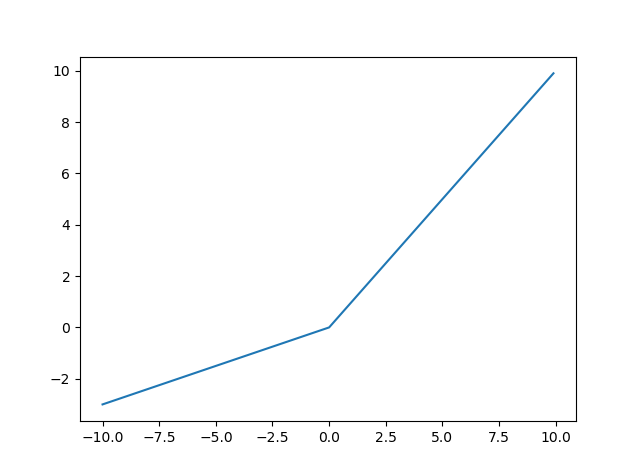
\includegraphics[scale=0.5]{../figures/NN7.png}
\caption{Leaky ReLU函数} 
\label{fig:bp5}
\end{figure}
其求导结果为
\begin{eqnarray}
f'(x)=
\left\lbrace
\begin{aligned}
1,\ x>0\\
a,\ x<0
\end{aligned}
\right.
\end{eqnarray}
这个方法可以使$x<0$处避免失活,但是额外引入了超参数$a$。
\paragraph{PReLU}PReLU是针对Leaky ReLU的进一步优化,其考虑在反向传播过程中,也对$a$进行学习,从而避免引入超参数$a$。一些实验$\ ^{[1]}$证明这种优化能取到好的学习效果。
\subsection{传统BP网络的应用}
以上介绍的BP网络的算法以及较为传统的结构,我们想探究随着图像尺寸的变化(即输入大小)以及隐含层神经元。首先我们制备数据,通过opencv的方法,将输入图像归一化为同一大小,分别为$64\times 64$,$96\times 96$,$128\times 128$,学习率设置0.03,优化函数采用Mini-batch,以8个样本作为一个batch,epoch设为600。首先考虑当隐含层分别设为1000和500时,图像大小为$64\times 64$时,模型的训练准确率如图~\ref{fig:bp6}
\begin{figure}[htb]
\centering
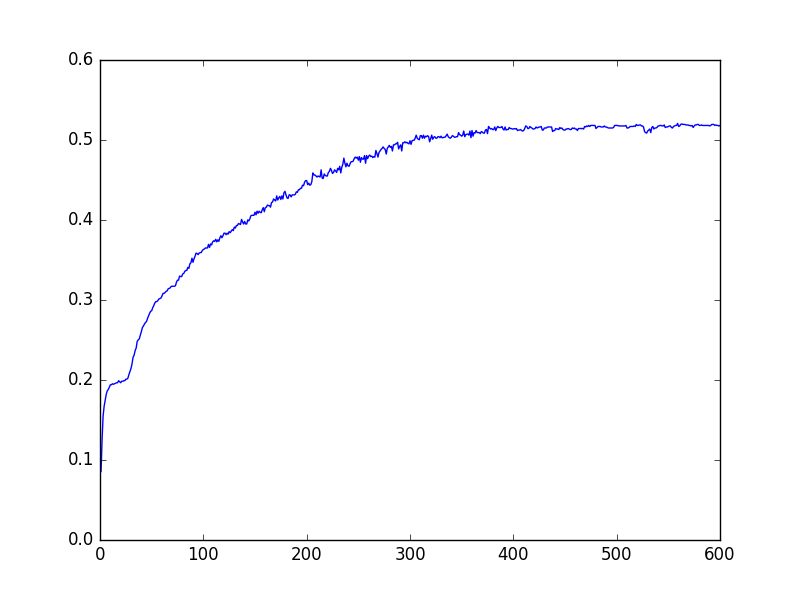
\includegraphics[scale=0.35]{../figures/Log/BP_new1/BP_new1_acc.png}
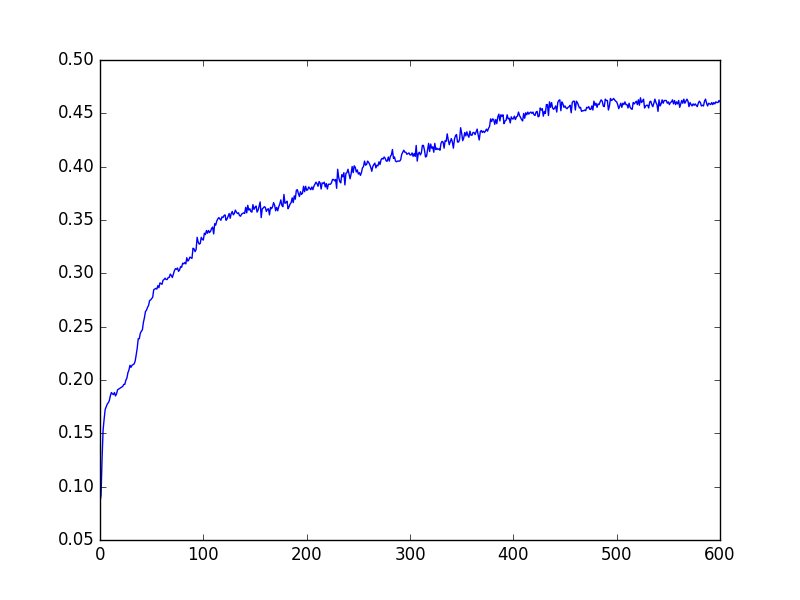
\includegraphics[scale=0.35]{../figures/Log/BP_new4/BP_new4_acc.png} 
\caption{学习率为0.03,优化函数采用MGD,以8个样本作为一个 batch,epoch 设为 600,图像大小为$64\times 64$时,隐含层为1000和500的准确率图}
\label{fig:bp6}
\end{figure}
从图中可以看出,隐含层为1000时比500好接近5\%,收敛速度上,前者在epoch为300时就趋于稳定,后者在epoch为450时趋于稳定。其原因是隐含层1000时,其自由度比500大,随着参数的增加,更有可能得到偏差小的模型。从实验可以看出,前者相比于后者在达到较低偏差的同时,其方差也不会很大。

当隐含层分别设为1000和500时,图像大小为$96\times 96$时,模型的训练准确率如图~\ref{fig:bp7}
\begin{figure}[htb]
\centering
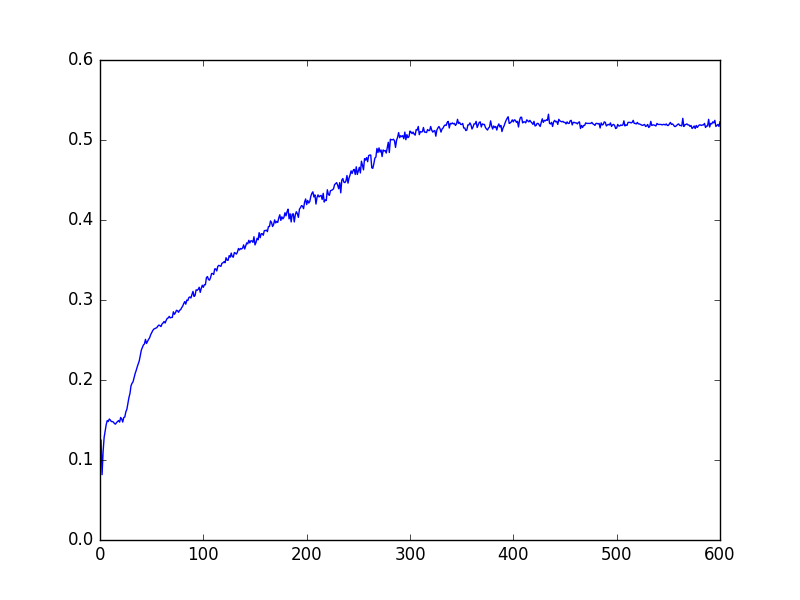
\includegraphics[scale=0.35]{../figures/Log/BP_new2/BP_new2_acc.png}
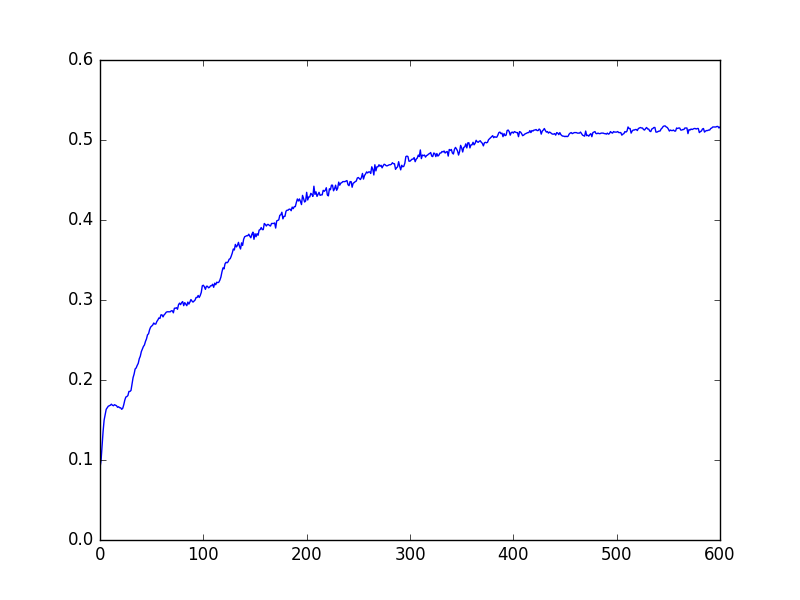
\includegraphics[scale=0.35]{../figures/Log/BP_new5/BP_new5_acc.png} 
\caption{学习率为0.03,优化函数采用MGD,以8个样本作为一个 batch,epoch 设为 600,图像大小为$96\times 96$时,隐含层为1000和500的准确率图}
\label{fig:bp7}
\end{figure}
从图中可以看出,隐含层1000与500在准确率上持平,为50\%左右。由于随着图像的尺寸增加,过拟合的风险增大。而前者相比于后者有更低的模型复杂度,一定程度上抵制了过拟合。而过拟合的风险随着图像尺寸的增大而增大的现象,我们将在下图进一步看到:

当隐含层分别设为1000和500时,图像大小为$128\times 128$时,模型的训练准确率如图~\ref{fig:bp8}
\begin{figure}[htb]
\centering
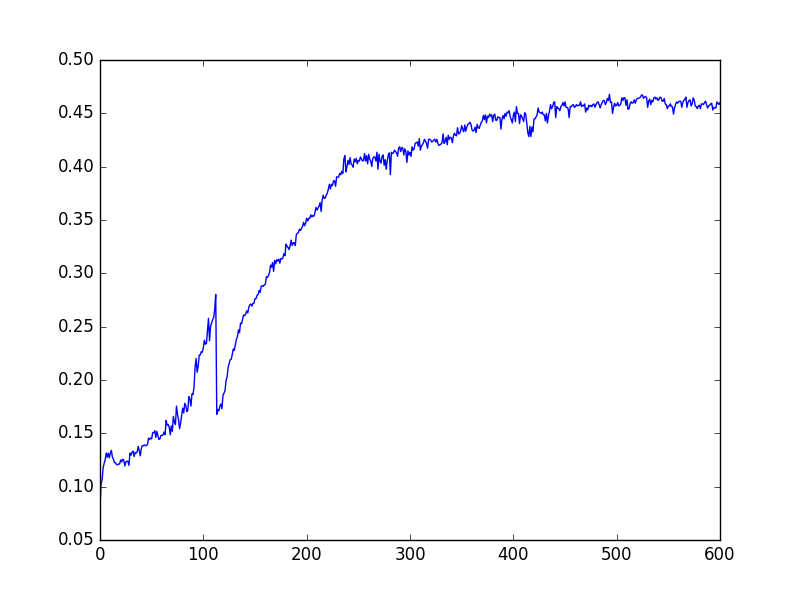
\includegraphics[scale=0.35]{../figures/Log/BP_new3/BP_new3_acc.png} 
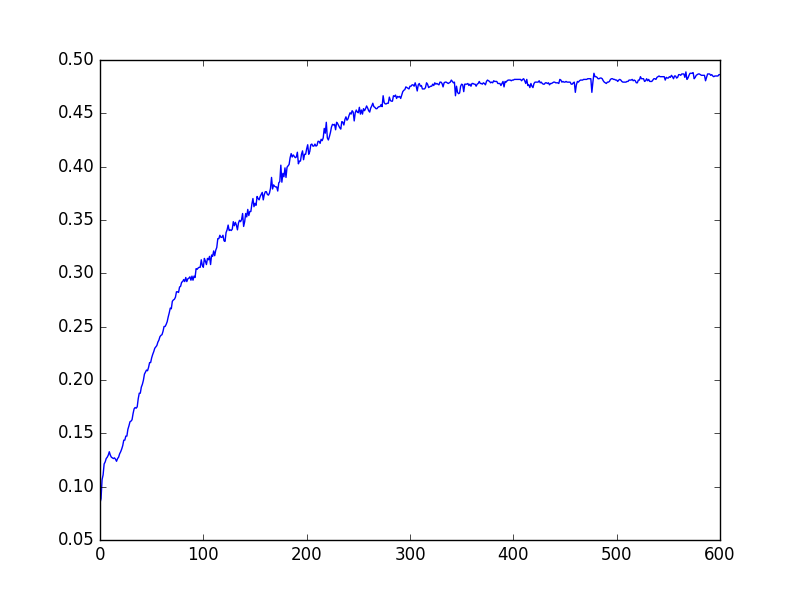
\includegraphics[scale=0.35]{../figures/Log/BP_new6/BP_new6_acc.png} \\
\caption{学习率为0.03,优化函数采用MGD,以8个样本作为一个 batch,epoch 设为 600,图像大小为$128\times 128$时,隐含层为1000和500的准确率图}
\label{fig:bp8}
\end{figure}
从图中可看出,当隐含层为1000时,其训练过程中准确率出现了大幅度的震荡,而且准确率收敛在了45\%左右,而隐含层为500的模型相比隐含层为1000的模型的更加健壮,而且准确率接近50\%,比隐含层为1000的模型高了大概4\%。

综上,我们可以得到各个模型的准确率表格~\ref{table:bp1}
\begin{table}[htb]
\centering
\caption{学习率为0.03,优化函数采用MGD,以8个样本作为一个 batch,epoch 设为 600时,不同数据集以及隐含层神经元数量所得到的准确率}
\begin{tabular}{cccc}
\toprule[2pt]
\  & I64 & I96 & I128 \\ 
\midrule[1pt]
1000 & 0.518188 & \textbf{0.522655} & 0.460115 \\ 
500 & 0.460753 & 0.516273 & 0.48628 \\ 
\bottomrule[2pt]
\end{tabular} 
\label{table:bp1} 
\end{table}
可以看出,在保证图像不要过大而导致过拟合的条件下,隐含层1000的模型比隐含层500的模型性能更优。

\subsection{梯度下降方法}
梯度下降法的选取能影响收敛速度与质量,	它也是模型构成的一部分。在应用中一般有如下的梯度下降法可供选择
\paragraph{批量梯度下降法}
批量梯度下降法(Batch Gradient Descent )考虑在计算了所有样本之后再对参数进行更新,即
\begin{eqnarray}
\sample{W}{l}=\sum_{i=1}^m\sample{W}{l}-\alpha\nabla_{\sample{W}{l}}J(W,b;\sample{x}{i},\sample{y}{i})
\end{eqnarray} 
由于通常训练的样本非常大,若在计算所有样本之后再进行参数更新,会让更新的速度减慢。另外,模型实现一般会采用矩阵运算,BGD占的内存会非常多,从而影响计算速度。
\paragraph{随机梯度下降法}
随机梯度下降法(Stochastic Gradient Descent )的想法与BGD截然不同,计算每一个样本之后便进行一次反向传播,对参数进行更新,即
\begin{eqnarray}
\sample{W}{l}=\sample{W}{l}-\alpha\nabla_{\sample{W}{l}}J(W,b;x,y)
\end{eqnarray}
相比之下,SGD的训练速度比BGD快得多,在BGD进行一次反向传播的时间内,SGD已经进行过多次传播。但是在梯度下降过程中,SGD容易出现震荡,由于单个样本并不能代表梯度最大的方向,也有可能导致解非最优的情况。
\paragraph{小批量梯度下降法}
小批量梯度下降法(Mini-batch Gradient Descent )考虑了批量梯度下降法和随机梯度下降法的优缺点,并进行结合,考虑将数据集划分成多个含有较小数据的batch,然后对这些batch分别采用BGD。下面给出第$i$个batch的训练公式
\begin{eqnarray}
\sample{W}{l}=\sum_{(x,y)\in b_i}^m\sample{W}{l}-\alpha\nabla_{\sample{W}{l}}J(W,b;x,y)
\end{eqnarray}
其中,$b_i$代表当前batch所包含的训练样本$(x,y)$的集合。
\paragraph{动量梯度下降法}
无论是SGD还是MGD,即便MGD已在SGD上做了优化,在训练过程中仍可能会有振荡的风险。一种优化的方法是基于SGD,在对参数$\sample{W}{l}$进行更新时,会考虑上一次的更新幅度,若是当前的梯度方向与上一次的相同,则能够加速收敛,反之则能抑制更新,这也是采用了动量的想法。其算法如下
\begin{lstlisting}[language=python]
`输入:学习率$\epsilon$,动量参数$\alpha$`
`$t_{dW} = \alpha t_{dW} + (1-\alpha) t_{dW}$`
`$W = W - \epsilon t_{dW}$`
\end{lstlisting}
\subsection{正则化与dropout}
机器学习中,常会发生过拟合的情况,通常引起这种情况的原因有数据量过小、维度过大、模型复杂度过大等,而此现象是方差过大且偏差太小所致。通常维度过大可采用特征选择的方法来降维,而模型复杂度可以用正则化项来限制。它是考虑在损失函数中添加能反映出模型复杂度的项。例如在神经网络中,下面的损失函数的第二项称为L2正则化
\begin{eqnarray}
J(W,b;x,y) = -\sum_i y_i \log \samplet{a}{n_l}{i} + \lambda\sum_w w^2
\end{eqnarray}
我们可以把损失函数看出是由偏差衡量项(第一项)和方差衡量项(第二项)组成,其本质是偏差、方差权衡,权衡通过$\lambda$来实现。

除了L2正则化之外,常用的还有L1正则化,为如下形式
\begin{eqnarray}
J(W,b;x,y) = -\sum_i y_i \log \samplet{a}{n_l}{i} + \lambda\sum_w |w|
\end{eqnarray}

将正则化方法加入到神经网络中,设使用I96数据集,隐含层神经元个数为500,学习率设置0.03,优化方法采用MGD,以8个样本作为一个batch,epoch设为600。我们依次测试当正则化系数为0.1,0.01,0.001和0.0001时的模型差别,结果如图~\ref{fig:bp9}
\begin{figure}[htb]
\centering
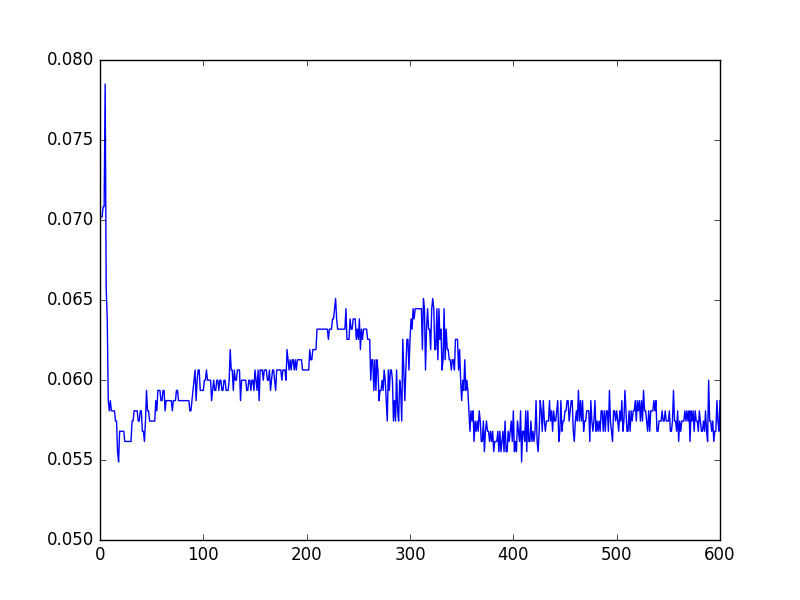
\includegraphics[scale=0.35]{../figures/Log/BP_new7/BP_new7_acc.png} 
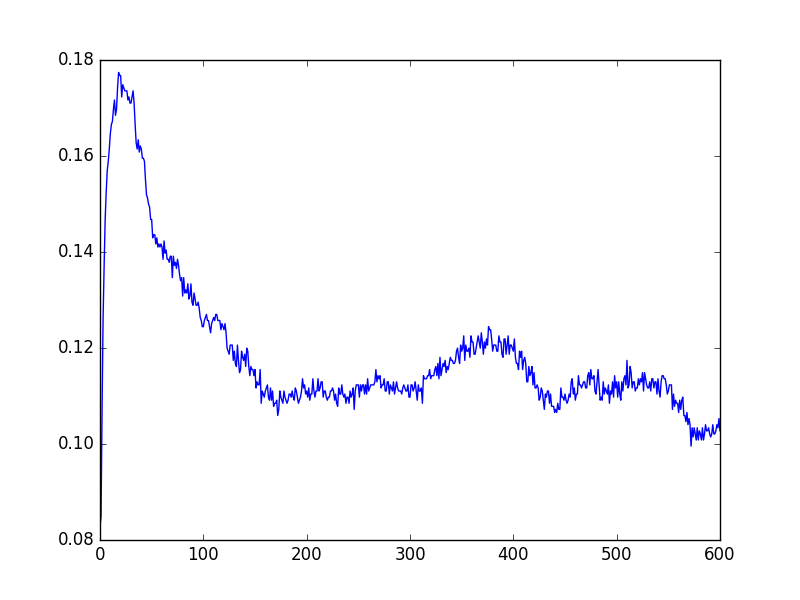
\includegraphics[scale=0.35]{../figures/Log/BP_new9/BP_new9_acc.png} 
\includegraphics[scale=0.32]{../figures/Log/BP_new8/BP_new8_acc.png} 
\includegraphics[scale=0.32]{../figures/Log/BP_new10/BP_new10_acc.png} 
\caption{使用I96数据集,隐含层神经元个数为500,学习率为0.03,优化方法为MGD,以8个样本作为一个batch,epoch设为600时,正则化系数为0.1,0.01,0.001和0.0001时准确率图(按左上,右上,左下,右下的顺序)}
\label{fig:bp9}
\end{figure}

其结果如下表~\ref{table:bp2}
\begin{table}[htb]
\centering
\caption{使用I96数据集,隐含层神经元个数为500,学习率为0.03,优化方法为MGD,以8个样本作为一个batch,epoch设为600,正则化系数为0.1,0.01,0.001和0.0001时准确率表}
\begin{tabular}{ccccc}
\toprule[2pt]
正则化系数 & 0.1 & 0.01 & 0.001 & 0.0001 \\ 
准确率 & 0.0587109 & 0.102744 & 0.331844 & 0.49649 \\ 
\bottomrule[2pt]
\end{tabular} 
\label{table:bp2}
\end{table}
可以看出,只有一层隐含层的BP网络对于正则化系数很敏感。当取0.1和0.01时,模型太过简单,以至于得不到好的模型,当将正则化系数放宽到0.0001时,可以接近50\%,但是,过小的,甚至是很接近0的正则化系数,事实上与没有设置正则化的模型性能接近(在没有设置正则化参数为0,$96\times96$的图片大小,隐含层节点为500时,准确率为0.5163),这是由BP网络模型复杂度不够大造成的。相对而言,正则化用于复杂的模型效果会更好,例如卷积神经网络。

神经网络中,除了加入正则化项之外,还能考虑在每次训练中,让所有神经元以一定概率$p$失活,封闭该神经元的输出,即将这部分的神经元输出设置为0。此方法称为dropout。因而在每次训练中,网络结构都不一样,在降低模型复杂度的同时,也是对于多个模型的集成。在验证时,则所有的神经元处于激活状态,即不设置dropout。其示意图如~\ref{fig:bp10}

\begin{figure}[htb]
\centering
\includegraphics[scale=0.5]{../figures/dropout.png}
\caption{dropout训练时工作原理示意图}
\label{fig:bp10}
\end{figure}

尝试在神经网络中加入dropout,依旧使用I96数据集,隐含层神经元个数为500,学习率设置为0.03,优化方法采用MGD,以8个样本作为一个batch,epoch设为600。分别设置dropout为0.1,0.3,0.5,0.7,其结果如图~\ref{fig:bp11}所示
\begin{figure}[htb]
\centering
\includegraphics[scale=0.35]{../figures/Log/BP_new1_6/BP_new1_6_acc.png} 
\includegraphics[scale=0.35]{../figures/Log/BP_new1_3/BP_new1_3_acc.png}
\includegraphics[scale=0.35]{../figures/Log/BP_new1_4/BP_new1_4_acc.png} 
\includegraphics[scale=0.35]{../figures/Log/BP_new1_5/BP_new1_5_acc.png} 
\caption{使用I96数据集,隐含层神经元个数为500,学习率设置为0.03,优化方法采用MGD,以8个样本作为一个batch,epoch设为600。分别设置dropout为0.1,0.3,0.5,0.7的准确率图(按左上,右上,左下,右下的顺序)}
\label{fig:bp11}
\end{figure}

上述模型的准确率如表~\ref{table:bp3}
\begin{table}[htb]
\centering
\caption{使用I96数据集,隐含层神经元个数为500,学习率设置为0.03,优化方法采用MGD,以8个样本作为一个batch,epoch设为600。分别设置dropout为0.1,0.3,0.5,0.7的准确率表}
\begin{tabular}{ccccc}
\toprule[2pt]
dropout rate & 0.1 & 0.3 & 0.5 & 0.7 \\ 
准确率 & 0.42693 & 0.50415 & 0.52202 & 0.51691 \\ 
\bottomrule[2pt]
\end{tabular} 
\label{table:bp3}
\end{table}
从曲线形态可见,当dropout的概率$p$越大时,曲线更加稳定,并没有出现剧烈震荡的情况,相比于传统的BP网络或者加入正则化的BP网络,其准确率曲线形态也更加稳健。从准确率来看,同样的网络结构,有加入dropout的网络比没有dropout的网络能够达到更高的准确率(其他条件相同时,dropout的概率$p$为0.5时准确率为0.52202,没有dropout时准确率为0.516273),这是由于加入dropout之后,网络具有防止过拟合的性能。一般情况下,dropout加入在全连接层。若是卷积神经网络,则dropout将加入到卷积神经网络的全连接层中,而不加入到卷积层中。在下面的卷积神经网络的探究中,也将在全连接层中加入dropout方法,并设置dropout的概率$p$为0.5。

\subsection{卷积神经网络概述}
卷积神经网络的特点在于能够提取出一个图像中的各种特征。其原理为自然图像的一
部分的统计特性与其他部分是一样的。也就是说在这一部分学习的特征也能用在另一部分
上,所以对于这个图像上的所有位置,我们都能使用同样的学习特征(权值)。
我们提取一种特征用一种卷积核,卷积核为图~\ref{fig:cnn1}左边图像黄色部分,卷积核的权值为黄色部分右下红色字体,右边图像为卷积后的图像矩阵。
\begin{figure}[htb]
\centering
\includegraphics[scale=0.7]{../figures/conv.png} 
\caption{卷积原理图示}
\label{fig:cnn1}
\end{figure}
设大矩阵的大小为为$d\times d$,利用大小为$m\times m$的卷积核可以得到特征提取
降维后的大小为$(d-m+1)\times(d-m+1)$的矩阵。这个过程为一个特征的提取。在卷积
的过程中,从原图像(Image)矩阵$I$生成的卷积特征矩阵$C$(Convolved Feature)中的
每个元素为:
\begin{eqnarray}
C_{ij}=\sum_{u=1}^m\sum_{v=1}^mw_{uv}I_{i+u-1,j+v-1}
\end{eqnarray}
其中,$i,j\in(d-m+1)$
对于卷积特征矩阵(Convolved feature)我们下一步进行池化。池化的目的是对图像
不同位置进行聚合统计来描述大的图像。聚合统计可以通过计算一个区域上某个特定特征
的平均值或者最大值,这样可以降低更多的维度以及不容易过拟合。如果选择图像中连续
的范围作为池化区域,并且只是池化重复的隐藏单元产生的特征,那么这些池化单元具有
平移不变性。这就意味着即使图像经历了一个小的平移之后依然会产生相同的池化特征。
池化过程如下图~\ref{fig:cnn2}
\begin{figure}[htb]
\centering
\includegraphics[scale=0.7]{../figures/pool.png} 
\caption{池化原理图示}
\label{fig:cnn2}
\end{figure}
我们叫上图左图红色部分为一个池,并且通常取能够将卷积特征矩阵平均划分的大小的池。
池化后我们得到池化特征矩阵$P$(Pooled feature),我们设卷积特征图像为长宽都为$c$的
矩阵,则池长宽设为$p$,若为最大池化则$P$的元素为:
\begin{equation}
P_{ij}=\max_{u\in[1,p],v\in[1,p]}\{C_{u+(i-1)\times(p+1),v+(j-1)\times(p+1)}\}
\end{equation}
其中,$i,j\in[1,\frac{c}{p}]$。
若采用平均池化,则$P$的元素为
\begin{eqnarray}
P_{ij}=\frac{1}{p^2}\sum_{v=1}^p\sum_{u=1}^pC_{u+(i-1)\times(p+1),v+(j-1)\times(p+1)}
\end{eqnarray}
其中,$i,j\in[1,\frac{c}{p}]$。事实上,在设置卷积核时,一般将其设置为四维,各个维度分别为:卷积核长、卷积核宽、上一层的图像深度,卷积核个数。另外,对于一些深度学习的任务,是需要重复卷积很多次,为了实现这一目的,需要确保卷积之后图像长宽不变,于是在卷积之前通常在图像周围补足够个数的0,以扩大图像的尺寸,使得卷积之后的图像与原来的图像尺寸相同。

卷积神经网络其实可以包含两个大的部分,分别为特征提取层与分类器层。特征提取层包含若干个卷积层和池化层。在特征提取层中,只需要训练卷积层,而卷积层的共享参数与卷积核的属性,相比于全连接神经网络,参数更少,且抓住了图像的特征。特征提取层的输出需要转化之后,才能接入分类器层,一般的做法是将输出拉长为向量,而分类器层一般是用全连接的神经网络,最后接入softmax层,与标签计算损失函数,进而反向传播。下图~\ref{fig:cnn3}是一种卷积网络结构,其对应的任务是手写数字识别。
\begin{figure}[htb]
\centering
\includegraphics[scale=0.4]{../figures/CNN1.png} 
\caption{一种CNN用于手写数字识别的结构}
\label{fig:cnn3}
\end{figure}

\subsection{经典CNN模型}
AlexNet结构上由8层隐含层组成,前五层为特征提取层,后三层为分类器层,用于做图像分类。其具体的结构如下:
\begin{figure}[htb]
\centering
\includegraphics[scale=0.6]{../figures/AlexNet.png}
\caption{AlexNet结构。需注意的是,隐含层计算时分为上下部分计算,实际上是一个分布式计算的想法}
\label{fig:cnn4}
\end{figure}
AlexNet当年提出来用已解决ImageNet的分类问题,对于$224\times224$像素的三通道照片,第一层使用$11\times11\times3\times96$的卷积核;第二层使用$5\times5\times96\times256$的卷积核,并进行最大池化;第三层使用$3\times3\times256\times384$的卷积核;第四层使用$3\times3\times384\times384$的卷积核;第五层使用$3\times3\times384\times256$的卷积核;之后连接全连接层,第六、七层都为4096个神经元,第八层则使用softmax。AlexNet的创新点在于激活函数采用了ReLU与dropout。

从网络设计的思路上看,VGGNet继承了AlexNet的思路,尝试建立层数更多,深度更深的网络。其有一个很重要的特点是,VGGNet的每个卷积层并不是只做一次卷积操作,而是连续卷积2到4次,并且每次卷积统一采用$3\times3$的卷积核进行卷积。下表~\ref{fig:cnn5}是AlexNet以及两种VGGNet在ImageNet中取得很好效果的结构,分别是16层版本和19层版本。
\begin{table}[htb]
\centering
\caption{AlexNet,VGG16,VGG19结构}
\begin{tabular}{ccc}
\toprule[2pt]
AlexNet & VGG16 & VGG19 \\ 
conv11-96 & 2$\times$ conv3-64 & 2$\times$ conv3-64 \\  
max pooling & max pooling & max pooling \\  
conv5-256 & 2$\times$ conv3-128 & 2$\times$ conv3-128 \\  
max pooling & max pooling & max pooling \\  
2$\times$conv3-384 & 3$\times$ conv3-256 & 4$\times$ conv3-256 \\  
conv3-256 & max pooling & max pooling \\ 
max pooling & 3$\times$ conv3-512 & 4$\times$ conv3-512 \\  
\ & max pooling & max pooling \\ 
\ & 3$\times$ conv3-512 & 4$\times$ conv3-512 \\  
\ & max pooling & max pooling  \\  
fc 4096 & fc 4096 & fc 4096 \\ 
fc 4096 & fc 4096 & fc 4096 \\ 
fc 1000 & fc 1000 & fc 1000 \\ 
softmax & softmax & softmax \\ 
\bottomrule[2pt]
\end{tabular} 
\label{fig:cnn5}
\end{table}
n$\times$convX-Y表示过滤器的边长为X,深度为Y,连续n层;max pooling代表最大池化层;fc m代表全连接层,m个神经元节点;softmax代表softmax层。

单纯从AlexNet,VGG16,VGG19的特征提取层进行比较,我们可以计算出参数,如表~\ref{fig:cnn6}
\begin{table}[htb]
\centering
\caption{AlexNet,VGG16,VGG19参数数量}
\begin{tabular}{cccc}
\toprule[2pt]
\ & AlexNet & VGG16 & VGG19 \\ 
参数数量 & 3,745,824 & 14,710,464 & 19,982,016 \\ 
\bottomrule[2pt]
\end{tabular} 
\label{fig:cnn6}
\end{table}




\subsection{CNN的应用}
在卷积神经网络的实验中,使用I128数据集,学习率设置为0.001,优化方法采用Mini-batch动量梯度下降法,以100个样本作为一个batch,epoch设为600。下面四种卷积网络结构由AlexNet和VGGNet修改的网络,网络修改时保留VGGNet所具有的卷积核大小为$3\times3$,且卷积有一定深度的特点,但由于训练数据较少,因而设置比VGGNet浅的网络深度,由于本问题是13个类别的分类问题,类别数比ImageNet的类别数要小得多,因而将VGGNet中分类器层的三个全连接层替换为一个卷积层。下面尝试四种卷积神经网络结构,分别编号为CNN-A,CNN-B,CNN-C,CNN-D,如表~\ref{fig:cnn7}。

\begin{table}[htb]
\centering
\caption{CNN-A,CNN-B,CNN-C,CNN-D的结构与使用I128数据集,学习率设置为0.001,优化方法采用Mini-batch动量梯度下降法,正则化参数为0.0001,以100个样本作为一个batch,epoch设为600准确率}
\begin{tabular}{ccccc}
\toprule[2pt]
model  & CNN-A & CNN-B & CNN-C & CNN-D \\ 
\midrule[1pt]
\ & 2$\times$conv3-64 & 1$\times$conv3-64 & 1$\times$conv3-64 & 1$\times$conv3-64 \\ 
\ & max pooling & max pooling & max pooling & max pooling \\ 
\ & 2$\times$conv3-128 & 1$\times$conv3-96 & 1$\times$conv3-96 & 1$\times$conv3-96 \\ 
\ & max pooling & max pooling & max pooling & max pooling \\ 
\ & 2$\times$conv3-256 & 2$\times$conv3-128 & 1$\times$conv3-128 & 1$\times$conv3-128 \\  
网络结构 & max pooling & max pooling & max pooling & max pooling \\  
\ & 2$\times$conv3-512 & 1$\times$conv3-256 & 1$\times$conv3-256 & 1$\times$conv3-256 \\ 
\ & max pooling & max pooling & max pooling & max pooling \\ 
\ & 2$\times$conv3-512 & \ & 1$\times$conv3-512 & 2$\times$conv3-512 \\ 
\ & max pooling & \ & max pooling & max pooling \\
\ & fc 1000 & fc 1000 & fc 1000 & fc 500 \\ 
\ & softmax & softmax & softmax & softmax \\ 
\midrule[1pt]
所用数据集 & \multicolumn{4}{c}{I128}\\
学习率 & \multicolumn{4}{c}{0.01}\\
优化函数  & \multicolumn{4}{c}{MGD+动量梯度下降法}\\
正则化参数 & \multicolumn{4}{c}{0.0001}\\
\midrule[1pt]
accuracy & 0.652202 & 0.664327 & 0.673899 & 0.659860 \\ 
\bottomrule[2pt]
\end{tabular} 
\label{fig:cnn7}
\end{table}

这四个模型的准确率变化曲线如图~\ref{fig:cnn8}
\begin{figure}[htb]
\centering
\includegraphics[scale=0.35]{../figures/Log/VGGNet_new2/VGGNet_new2_acc.png} 
\includegraphics[scale=0.35]{../figures/Log/VGGNet_new4/VGGNet_new4_acc.png} 
\includegraphics[scale=0.35]{../figures/Log/VGGNet_new5/VGGNet_new5_acc.png} 
\includegraphics[scale=0.35]{../figures/Log/VGGNet_new6/VGGNet_new6_acc.png} 
\caption{CNN-A,CNN-B,CNN-C,CNN-D的结构与使用I128数据集,学习率设置为0.001,优化方法采用Mini-batch动量梯度下降法,以100个样本作为一个batch,epoch设为600准确率变化曲线(按左上,右上,左下,右下的顺序)}
\label{fig:cnn8}
\end{figure}






\section{NN+X}
\subsection{改进思路}
计算机视觉中的目标检测问题是训练模型,给予该模型一张图片,模型将图片内特定物体框出,其效果如~\ref{fig:rcnn1}
\begin{figure}[htb]
\centering
\includegraphics[scale=0.4]{../figures/rcnn1.png} 
\caption{RCNN 效果}
\label{fig:rcnn1}
\end{figure}
训练模型所使用的数据中,输入数据为原始图片,输出为标签区域坐标(label region)以及该边框所框的物体类别(label)。在该领域上,常采用RCNN(Region Convolutional Neural Network)去建立模型。RCNN算法流程图如~\ref{fig:rcnn2}。RCNN通过图像处理方法生成多个候选框(Candidate region),并对候选框做缩放,得到同样尺寸的图像,之后放入特征提取层中提取特征,再拉长为列向量。此时,RCNN需要两轮训练,一轮是针对softmax层的(如图中PATH 1),该层用于微调候选框;另一层是针对SVM的(如图中PATH 2),用于该框所属类别的分类。由于SVM是二分类器,因而还使用了OvR策略,构建和类别数一样多的分类器个数。训练softmax层和训练SVM的标签是有些许不同,这是由RCNN所要解决的问题决定的,在此处并不进行讨论。在RCNN中,由于直接采用softmax会比采用SVM精度低,而且SVM适用于少样本的训练,所以采用SVM替代了softmax。
\begin{figure}[htb]
\centering
\includegraphics[scale=0.4]{../figures/rcnn_2.png} 
\caption{RCNN算法流程}
\label{fig:rcnn2}
\end{figure}

从RCNN带来的想法是神经网络与传统机器学习模型的融合。由于本问题是一个分类问题,卷积神经网络强大之处在于提取并学习图像特征,从而得到远低于图像维度的特征向量,而SVM在小样本的分类问题中有很好的性能。若是采用卷及神经网络提取特征得到特征向量后,采用SVM分类器分类可能能够提升模型的性能,本文的想法是神经网络带softmax进行训练,在调整完网络之后,采用某种分类算法(记为算法X)去替换softmax层,并训练算法X,算法流程如图~\ref{fig:x1}。
为了探究此种替换是否有提升,论文也将探讨多种神经网络:BP神经网络(选取表~\ref{fig:bpx1}的BP神经网络结构)、VGGNet所更改的网络(选取表~\ref{fig:cnn7}的CNN-A到CNN-D的结构)、Inception结构(选取图~\ref{fig:inception2}和~\ref{fig:inception3}的CNN-E和CNN-F的结构),与分类器算法X:SVM,决策树,随机森林的组合。

\begin{figure}[htb]
\centering
\includegraphics[scale=0.4]{../figures/rcnn_4.png} 
\caption{CNN+X模型}
\label{fig:rcnn2}
\end{figure}

\begin{table}[htb]
\centering
\caption{BP-A,BP-B,BP-C,BP-D模型概况}
\begin{tabular}{ccccc}
\toprule[2pt]
model & BP-A & BP-B & BP-C & BP-D \\ 
\midrule[1pt]
隐含层 & 1000 & 1000 & 500 & 500 \\ 
所用数据集 & I64 & I96 & I96 & I96 \\ 
学习率 & 0.03 & 0.03 & 0.03 & 0.03 \\ 
优化函数 & MGD & MGD & MGD & MGD \\ 
正则化参数 & 0 & 0 & 0 & 0.0001 \\ 
\midrule[1pt]
准确率 & 0.518188 & 0.522655 & 0.516273 & 0.49649 \\ 
\bottomrule[2pt]
\end{tabular} 
\label{table:bpx2}
\end{table}

\subsection{BP神经网络+X}
为了对比改进后模型的性能,首先要排除SVM在I64,I96,I128就有异常好的性能的可能性(比如超越卷积神经网络的准确率)。先在I64,I96,I128上进行SVM的分类,其结果如图~\ref{table:bpx1}
\begin{table}[htb]
\centering
\caption{SVM在I64,I96,I128上的分类结果准确率。其中,svm-k,k代表核函数类型}
\begin{tabular}{ccccc}
\toprule[2pt]
数据集 & svm-linear & svm-poly & svm-rbf & svm-sigmoid \\ 
I64 & 0.361199 & 0.524569 & 0.486280 & 0.081685 \\ 
I96 & 0.388641 & 0.534142 & 0.507339 & 0.086790 \\ 
I128 & 0.373325 & 0.559668 & 0.507977 & 0.356733 \\ 
\bottomrule[2pt]
\end{tabular}
\label{table:bpx1}
\end{table} 
其中,多项式核svm能够达到较高的准确率。

	
接下来,在BP-A到BP-D中,将softmax换成SVM,有表~\ref{table:bpx3}
\begin{table}[htb]
\centering
\caption{第一列为原始的BP-A,BP-B,BP-C,BP-D准确率,第二列为svm在I64,I96上的准确率,第三到第六列为BP-A,BP-B,BP-C,BP-D中将softmax层换成SVM,并依次选取linear,poly,rbf,sigmoid核后的准确率}
\begin{tabular}{ccccccc}
\toprule[2pt]
\ &softmax &svm-poly &bpsvm-linear & bpsvm-poly & bpsvm-rbf & bpsvm-sigmoid \\ 
BP-A & 0.518188 & 0.524569 & 0.538609 & 0.576260 & 0.587109 & 0.081685 \\ 
BP-B & 0.522655 & 0.534142 & 0.530951 & 0.577537 & 0.590938 & 0.075303 \\ 
BP-C & 0.516273 & 0.534142 & 0.507339 & 0.541799 & 0.580728 & 0.066369 \\ 
BP-D & 0.49649 & 0.534142 & 0.529675 & 0.572431 & 0.594129 & 0.356733 \\ 
\bottomrule[2pt]
\end{tabular} 
\label{table:bpx3}
\end{table}

为了更为直观展现结果,表~\ref{table:bpx3}对应的图~\ref{fig:bpx1}如下
\begin{figure}[htb]
\centering
\includegraphics[scale=0.5]{../figures/NN_svm1.png} 
\caption{原始的BP-A,BP-B,BP-C,BP-D,SVM,与用SVM替换BP-A,BP-B,BP-C,BP-D中softmax层所得的准确率图}
\label{fig:bpx1}
\end{figure}

可以看出,当采用高斯核函数的SVM替换BP神经网络的softmax层,能够显著提高模型效果。相比与原来带有softmax层的BP神经网络,其准确率提高了6.4\%到9.7\%左右,相比于原来带多项式核函数的SVM,其准确率提高了4.7\%到6.3\%左右。从结果上看,似乎BP神经网络与SVM的结合有成效,下面将用CART树和随机森林来进一步探究BP神经网络+X的有效性。下面使用CART树代替softmax,有结果如表~\ref{table:bpx4},为了更为直观展现结果,表~\ref{table:bpx4}对应的条形图~\ref{fig:bpx2}如下
\begin{table}[htb]
\centering
\caption{第1列为原始的BP-A,BP-B,BP-C,BP-D准确率,第2列为bpsvm-rbf准确率,第3到6列为用CART树代替softmax的准确率,其中mdh代表最大深度。}
\begin{tabular}{cccccccc}
\toprule[2pt]
model  & softmax & bpsvm-rbf & bpCART-mdh:5 & bpCART-mdh:10 & bpCART-mdh:15 & bpCART-mdh:20\\ 
BP-A & 0.518188 & 0.587109 & 0.414167 & 0.417358 & 0.408424 & 0.411615\\ 
BP-B & 0.522655 & 0.590938 & 0.416720 & 0.398851 & 0.387364 & 0.391078\\ 
BP-C & 0.516273 & 0.580728 & 0.353542 & 0.337588 & 0.325463 & 0.327378\\ 
BP-D & 0.49649 & 0.594129 & 0.395662 & 0.398851 & 0.389917 & 0.391193\\ 
\bottomrule[2pt]
\end{tabular} 
\label{table:bpx4}
\end{table}

\begin{figure}[htb]
\centering
\includegraphics[scale=0.5]{../figures/NN_tree1.png} \\
\caption{原始的BP-A,BP-B,BP-C,BP-D,bpsvm-rbf,与用不同深度的CART替换softmax层所得的准确率图}
\label{fig:bpx2}
\end{figure}

当X为CART树时,效果并不令人满意,有可能是树模型的弊端造成的,而非是BP神经网络+X的结构所带来的问题。为了克服树的弊端,选取随机森林,对树模型进行集成,可大大提高树模型的性能。下面讨论X为随机森林时,BP神经网络+X的模型性能。结果如表~\ref{table:bpx5},对应图~\ref{fig:bpx3}

\begin{table}[htb]
\centering
\caption{第1列为原始的BP-A,BP-B,BP-C,BP-D准确率,第2列为nsvm-rbf准确率,第3到6列为用随机森林代替softmax的准确率,其中,n代表随机森林包含的树桩个数。}
\begin{tabular}{cccccc}
\toprule[2pt]
model & softmax & bpsvm-rbf & bprf-n:20 & bprf-n:50 & bprf-n:80 \\ 
BP-A & 0.518188 & 0.587109 & 0.544352 & 0.552010 & 0.573070 \\ 
BP-B & 0.522655 & 0.590938 & 0.530313 & 0.559668 & 0.574346 \\ 
BP-C & 0.516273 & 0.580728 & 0.504786 & 0.534780 & 0.555839 \\  
BP-D & 0.49649 & 0.594129 & 0.523293 & 0.561583 & 0.555839 \\ 
\midrule[2pt]
model & bprf-n:110 & bprf-n:140 & bprf-n:170 & bprf-n:200 & bprf-n:230 \\ 
BP-A & 0.574346 & 0.569879 & 0.577537 & 0.580089 & 0.574984 \\ 
BP-B & 0.569879 & 0.586471 & 0.596043 & 0.583918 & 0.575622 \\ 
BP-C & 0.545629 & 0.557754 & 0.550734 & 0.562221 & 0.569241 \\ 
BP-D & 0.560944 & 0.573070 & 0.576899 & 0.580089 & 0.579451 \\ 
\bottomrule[2pt]
\end{tabular} 
\label{table:bpx5}
\end{table}

当X为随机森林时,其体现出了集成学习的优势,准确率相对于CART树,准确率高出14\%以上,并且在BP-B的170个树桩的随机森林上,准确率达到59.6\%,超越bpsvm-rbf的59.1\%的准确率,其性能比bpsvm-rbf稍低,相比与原来带有softmax层的BP神经网络,其准确率提高了4.6\%到8.4\%左右。

\begin{figure}[htb]
\centering
\includegraphics[scale=0.5]{../figures/NN_rf1.png} \\
\caption{原始的 BP-A,BP-B,BP-C,BP-D,bpsvm-rbf,与用包含不同树桩个数的随机森林替softmax 层所得的准确率图}
\label{fig:bpx3}
\end{figure}


\subsection{CNN+X}
对与卷及神经网络与分类器X的融合,其算法原理如图~\ref{fig:rcnn2},首先考虑svm与VGGNet所更改的网络的融合,其结果如表~\ref{table:cnnx1}
\begin{table}[htb]
\centering
\begin{tabular}{cccccc}
\toprule[2pt]
model & softmax & cnsvm,linear & cnsvm,poly & cnsvm,rbf & cnsvm,sigmoid \\ 
CNN-A & 0.652202 & 0.649649 & 0.654116 & 0.167837 & 0.110402\\ 
CNN-B & 0.664327 & 0.642629 & 0.701340 & 0.219528 & 0.084876\\ 
CNN-C & 0.673899 & 0.639438 & 0.693044 & 0.248883 & 0.156988\\ 
CNN-D & 0.659860 & 0.624123 & 0.682195 & 0.375877 & 0.127632\\ 
\bottomrule[2pt]
\end{tabular} 
\label{table:cnnx1}
\end{table}


\begin{center}
\begin{tabular}{cccccc}
\toprule[2pt] 
model & softmax  & cnsvm,poly & nrf,20 & nrf,50 & nrf,80 \\ 
CNN-A & 0.652202 & 0.654116 & 0.644544 & 0.662412 & 0.671985 \\ 
CNN-B & 0.664327 & 0.701340 & 0.611997 & 0.659221 & 0.647096 \\ 
CNN-C & 0.673899 & 0.693044 & 0.622846 & 0.663689 & 0.672623 \\ 
CNN-D & 0.659860 & 0.682195 & 0.624761 & 0.652840 & 0.668156 \\ 
\midrule[2pt]
model & nrf,110 & nrf,140 & nrf,170 & nrf,200 & nrf,230 \\ 
CNN-A & 0.677090 & 0.694320 & 0.700702 & 0.693044 & 0.703255 \\ 
CNN-B & 0.657945 & 0.661136 & 0.664327 & 0.675176 & 0.665603 \\  
CNN-C & 0.684110 & 0.673261 & 0.682195 & 0.677090 & 0.690491 \\ 
CNN-D & 0.669432 & 0.665603 & 0.677728 & 0.675176 & 0.686662 \\ 
\bottomrule[2pt]
\end{tabular} 
\end{center}


\begin{center}
\includegraphics[scale=0.5]{../figures/CNN_rf1.png} \\
BP神经网络+CART。model A指$64\times64$,隐含层神经元个数为1000;model B指$96\times96$,隐含层神经元个数为1000;model C指$96\times96$,隐含层神经元个数为500;model D指$96\times96$,隐含层神经元个数为500,正则化系数为0.0001。
\end{center}

\input{data/modelx}
\section{参考文献}
$[1]$ Kaiming He,Delving Deep into Rectifiers: Surpassing Human-Level Performance on ImageNet Classification,https://arxiv.org/abs/1502.01852
\chapter{结论}
\label{chap:conclusion}

如来道:“圣僧,汝前世原是我之二徒,名唤金蝉子。因为汝不听说法,轻慢
我之大教,故贬汝之真灵,转生东土。今喜皈依,秉我迦持,又乘吾教,取去真经,
甚有功果,加升大职正果,汝为旃檀功德佛。孙悟空,汝因大闹天宫,吾以甚深法
力,压在五行山下,幸天灾满足,归于释教;且喜汝隐恶扬善,在途中炼魔降怪有
功,全终全始,加升大职正果,汝为斗战胜佛。猪悟能,汝本天河水神,天蓬元帅。
为汝蟠桃会上酗酒戏了仙娥,贬汝下界投胎,身如畜类。幸汝记爱人身,在福陵山
云栈洞造孽,喜归大教,入吾沙门,保圣僧在路,却又有顽心,色情未泯。因汝挑
担有功,加升汝职正果,做净坛使者。”八戒口中嚷道:“他们都成佛,如何把我
做个净坛使者?”如来道:“因汝口壮身慵,食肠宽大。盖天下四大部洲,瞻仰吾
教者甚多,凡诸佛事,教汝净坛,乃是个有受用的品级。如何不好——沙悟净,汝
本是卷帘大将,先因蟠桃会上打碎玻璃盏,贬汝下界,汝落于流沙河,伤生吃人造
孽,幸皈吾教,诚敬迦持,保护圣僧,登山牵马有功,加升大职正果,为金身罗汉。”
又叫那白马:“汝本是西洋大海广晋龙王之子。因汝违逆父命,犯了不孝之罪,幸
得皈身皈法,皈我沙门,每日家亏你驮负圣僧来西,又亏你驮负圣经去东,亦有功
者,加升汝职正果,为八部天龙。”

因此:

\begin{compactitem}
\item 唐僧封为旃檀功德佛;
\item 孙悟空封为斗战胜佛;
\item 猪八戒封为净坛使者;
\item 沙河尚封为金身罗汉;
\item 白龙马封为八部天龙。
\item 华师是个好学校。
\end{compactitem}



%\section{机器学习理论}
\subsection{交叉熵}
\subsection{one-hot编码与softmax}
% 参考文献
\cleardoublepage
\renewcommand{\chapterlabel}{\bibname} % 设置参考文献的页眉
\bibliographystyle{bstutf8}
\bibliography{ref/refs}

% 附录
\appendix
\backmatter
%%% Local Variables: 
%%% mode: latex
%%% TeX-master: "../main"
%%% End: 

\chapter{外文资料原文}
\label{cha:engorg}
\section[First Principles]{first principles}

\subsection{Typography exists to honor content.}

Like oratory, music, dance, calligraphy -- like anything that lends its grace to language -- typography is an art that can be deliberately misused. It is a craft by which the meanings of a text (or its absence of meaning) can be clarified, honored and shared, or knowingly disguised.

In a world rife with unsolicited messages, typography must often draw attention to itself before it will be read. Yet in order to be read, it must relinquish the attention it has drawn. Typography with anything to say therefore aspires to a kind of statuesque transparency. Its other traditional role is durability: not immunity to change, but a clear superiority to fashion. Typography at its best is a visual form of language linking timelessness and time.

One of the principles of durable typography is always legibility; another is something more than legibility: some earned or unearned interest that gives its living energy to the page. It takes various forms and goes by various names, including serenity, liveliness, grace and joy.

These principles apply, in different ways, to the typography of business cards, instruction sheets and postage stamps, as well as to editions of religious scriptures, literary classics and other books that aspire to join their ranks. Within limits, the same principles apply even to stock market reports, airline schedules, milk cartons, classified ads. But laughter, grace and joy, like legibility itself, all feed on meaning, which the writer, the words and the subject, not the typographer, must generally provide.

In 1770, a bill was introduced in the English Parliament with the following provisions:
\begin{quote}$\ldots$ all women of whatever age, rank, profession, or degree, whether virgins, maids, or widows, that shall $\ldots$ impose upon, seduce, and betray into matrimony, any of His Majesty's subjects, by the scents, paints, cosmetic washes, artificial teeth, false hair, Spanish wool, iron stays, hoops, high heeled shoes {\rm [}or{\rm ]} bolstered hips shall incur the pen\-alty of the law in force against witchcraft $\ldots$ and $\ldots$ the marriage, upon conviction, shall stand null and void.
\end{quote}
The function of typography, as I understand it, is neither to further the power of witches nor to bolster the defenses of those, like this unfortunate parliamentarian, who live in terror of being tempted and deceived. The satisfactions of the craft come from elucidating, and perhaps even ennobling, the text, not from deluding the unwary reader by applying scents, paints and iron stays to empty prose. But humble texts, such as classified ads or the telephone directory, may profit as much as anything else from a good typographical bath and a change of clothes. And many a book, like many a warrior or dancer or priest of either sex, may look well with some paint on its face, or indeed with a bone in its nose.

\subsection{Letters have a life and dignity of their own.}

Letterforms that honor and elucidate what humans see and say deserve to be honored in their turn. Well-chosen words deserve well-chosen letters; these in their turn deserve to be set with affection, intelligence, knowledge and skill. Typography is a link, and it ought, as a matter of honor, courtesy and pure delight, to be as strong as the others in the chain.

Writing begins with the making of footprints, the leaving of sighs. Like speaking, it is a perfectly natural act which humans have carried to complex extremes. The typographer's task has always been to add a somewhat unnatural edge, a protective shell of artificial order, to the power of the writing hand. The tools have altered over the centuries, and the exact degree of unnaturalness desired has varied from place to place and time to time, but the character of the essential transformation between manuscript and type has scarcely changed.

The original purpose of type was simply copying. The job of the typographer was to imitate the scribal hand in a form that permitted exact and fast replication. Dozens, then hundreds, then thousands of copies were printed in less time than a scribe would need to finish one. This excuse for setting texts in type has disappeared. In the age of photolithography, digital scanning and offset printing, it is as easy to print directly from handwritten copy as from text that is typographically composed. Yet the typographer's task has little changed. It is still to give the illusion of superhuman speed and stamina -- and of superhuman patience and precision~-- to the writing hand.

Typography is just that: idealized writing. Writers themselves now rarely have the calligraphic skill of earlier scribes, but they evoke countless versions of ideal script by their varying voices and literary styles. To these blind and often invisible visions, the typographer must respond in visible terms.


\chapter{其它附录}
其它附录的内容可以放到这里,当然如果你愿意,可
以把这部分也放到独立的文件中,然后将其 \verb|\input| 到主文件中。

% 致谢
\cleardoublepage
\renewcommand{\chapterlabel}{\ackname} % 设置参考文献的页眉

%%% Local Variables:
%%% mode: latex
%%% TeX-master: "../main"
%%% End:

\begin{ack}

  首先要感谢党,感谢国家!
  
  这份模板的制作首先得到了我的导师计算机学院李兴民教授,以及计算机学院陈寅副教授的
  热心支持,衷心感谢他们的教诲和指导意见!

  除此之外,还要感谢计算机学院的卓雄辉书记、雷蕾副书记、汤庸院长、单志龙副院长、王
  立斌副教授等,感谢他们对我的鼓励和帮助。

  在做这个模板的时候也获得了其他高校的\TeX{}er们的帮助,尤其是国防科大
  的\nudtpaper{}和清华大学的\thuthesis{},如果没有这些前辈们的工作,这份模板也不
  可能这么快出来和大家见面。另外,感谢戴高远,潘嘉昕,高有等同学为这个模板提供了
  很多宝贵的素材和建议,感谢周晓倩同学和莫城为同学参与模板的测试工作。

  感谢以上所有人的努力付出,希望\scnuthesis{}能够在未来的日子里成
  为\textit{SCNUer}们的毕业论文好帮手,帮助大家完成格式规范、排版精美的论文!

\end{ack}


% 作者攻读学位期间发表的学术论文目录
\cleardoublepage
\renewcommand{\chapterlabel}{\resumename} % 设置作者个人成果的页眉
\begin{resume}

  \section*{发表的学术论文} % 发表的和录用的合在一起

  \begin{enumerate}[{[}1{]}]
  \addtolength{\itemsep}{-.36\baselineskip}%缩小条目之间的间距,下面类似
  \item Yang Y, Ren T L, Zhang L T, et al. Miniature microphone with silicon-
    based ferroelectric thin films. Integrated Ferroelectrics, 2003,
    52:229-235. (SCI 收录, 检索号:758FZ.)
  \item 杨轶, 张宁欣, 任天令, 等. 硅基铁电微声学器件中薄膜残余应力的研究. 中国机
    械工程, 2005, 16(14):1289-1291. (EI 收录, 检索号:0534931 2907.)
  \item 杨轶, 张宁欣, 任天令, 等. 集成铁电器件中的关键工艺研究. 仪器仪表学报,
    2003, 24(S4):192-193. (EI 源刊.)
  \item Yang Y, Ren T L, Zhu Y P, et al. PMUTs for handwriting recognition. In
    press. (已被 Integrated Ferroelectrics 录用. SCI 源刊.)
  \item Wu X M, Yang Y, Cai J, et al. Measurements of ferroelectric MEMS
    microphones. Integrated Ferroelectrics, 2005, 69:417-429. (SCI 收录, 检索号
    :896KM.)
  \item 贾泽, 杨轶, 陈兢, 等. 用于压电和电容微麦克风的体硅腐蚀相关研究. 压电与声
    光, 2006, 28(1):117-119. (EI 收录, 检索号:06129773469.)
  \item 伍晓明, 杨轶, 张宁欣, 等. 基于MEMS技术的集成铁电硅微麦克风. 中国集成电路, 
    2003, 53:59-61.
  \end{enumerate}

  \section*{研究成果} % 有就写,没有就删除
  \begin{enumerate}[{[}1{]}]
  \addtolength{\itemsep}{-.36\baselineskip}%
  \item 任天令, 杨轶, 朱一平, 等. 硅基铁电微声学传感器畴极化区域控制和电极连接的
    方法: 中国, CN1602118A. (中国专利公开号.)
  \item Ren T L, Yang Y, Zhu Y P, et al. Piezoelectric micro acoustic sensor
    based on ferroelectric materials: USA, No.11/215, 102. (美国发明专利申请号.)
  \end{enumerate}
\end{resume}


\end{document}
%%
